% Latex header for doxygen 1.8.13
\documentclass[twoside]{article}

% Packages required by doxygen
\usepackage{fixltx2e}
\usepackage{calc}
\usepackage{doxygen}
\usepackage[export]{adjustbox} % also loads graphicx
\usepackage{graphicx}
\usepackage[utf8]{inputenc}
\usepackage{makeidx}
\usepackage{multicol}
\usepackage{multirow}
\PassOptionsToPackage{warn}{textcomp}
\usepackage{textcomp}
\usepackage[nointegrals]{wasysym}
\usepackage[table]{xcolor}

% NLS support packages
\usepackage[french]{babel}

% Font selection
\usepackage[T1]{fontenc}
\usepackage[scaled=.90]{helvet}
\usepackage{courier}
\usepackage{amssymb}
\usepackage{sectsty}
\renewcommand{\familydefault}{\sfdefault}
\allsectionsfont{%
  \fontseries{bc}\selectfont%
  \color{darkgray}%
}
\renewcommand{\DoxyLabelFont}{%
  \fontseries{bc}\selectfont%
  \color{darkgray}%
}
\newcommand{\+}{\discretionary{\mbox{\scriptsize$\hookleftarrow$}}{}{}}

% Page & text layout
\usepackage{geometry}
\geometry{%
  a4paper,%
  top=2cm,%
  bottom=2cm,%
  left=1.2cm,%
  right=1.2cm%
}
\tolerance=750
\hfuzz=15pt
\hbadness=750
\setlength{\emergencystretch}{15pt}
\setlength{\parindent}{0cm}
\setlength{\parskip}{3ex plus 2ex minus 2ex}
\makeatletter
\renewcommand{\paragraph}{%
  \@startsection{paragraph}{4}{0ex}{-1.0ex}{1.0ex}{%
    \normalfont\normalsize\bfseries\SS@parafont%
  }%
}
\renewcommand{\subparagraph}{%
  \@startsection{subparagraph}{5}{0ex}{-1.0ex}{1.0ex}{%
    \normalfont\normalsize\bfseries\SS@subparafont%
  }%
}
\makeatother

% Headers & footers
\usepackage{fancyhdr}
\pagestyle{fancyplain}
\fancyhead[LE]{\fancyplain{}{\bfseries\thepage}}
\fancyhead[CE]{\fancyplain{}{}}
\fancyhead[RE]{\fancyplain{}{\bfseries\leftmark}}
\fancyhead[LO]{\fancyplain{}{\bfseries\rightmark}}
\fancyhead[CO]{\fancyplain{}{}}
\fancyhead[RO]{\fancyplain{}{\bfseries\thepage}}
\fancyfoot[LE]{\fancyplain{}{\bfseries\scriptsize Gr\+O\+Om 0.\+2}}
\fancyfoot[CE]{\fancyplain{}{}}
\fancyfoot[RE]{\fancyplain{}{\bfseries\scriptsize B\+T\+S S\+N\+I\+R La\+Salle Avignon 2020 }}
\fancyfoot[LO]{\fancyplain{}{\bfseries\scriptsize B\+T\+S S\+N\+I\+R La\+Salle Avignon 2020 }}
\fancyfoot[CO]{\fancyplain{}{}}
\fancyfoot[RO]{\fancyplain{}{\bfseries\scriptsize Gr\+O\+Om 0.\+2}}
\renewcommand{\footrulewidth}{0.4pt}
\renewcommand{\sectionmark}[1]{%
  \markright{\thesection\ #1}%
}

% Indices & bibliography
\usepackage{natbib}
\usepackage[titles]{tocloft}
\setcounter{tocdepth}{3}
\setcounter{secnumdepth}{5}
\makeindex

% Hyperlinks (required, but should be loaded last)
\usepackage{ifpdf}
\ifpdf
  \usepackage[pdftex,pagebackref=true]{hyperref}
\else
  \usepackage[ps2pdf,pagebackref=true]{hyperref}
\fi
\hypersetup{%
  colorlinks=true,%
  linkcolor=blue,%
  citecolor=blue,%
  unicode%
}

% Custom commands
\newcommand{\clearemptydoublepage}{%
  \newpage{\pagestyle{empty}\cleardoublepage}%
}

\usepackage{caption}
\captionsetup{labelsep=space,justification=centering,font={bf},singlelinecheck=off,skip=4pt,position=top}

%===== C O N T E N T S =====

\begin{document}

% Titlepage & ToC
\hypersetup{pageanchor=false,
             bookmarksnumbered=true,
             pdfencoding=unicode
            }
\pagenumbering{alph}
\begin{titlepage}
\vspace*{7cm}

\begin{center}%
{\LARGE Gr\+O\+Om}\\
\vspace*{1cm}
{\large version 0.\+2}\\
\vspace*{1cm}
{\large B\+T\+S S\+N\+I\+R La\+Salle Avignon 2020}\\
\end{center}
\end{titlepage}
\pagenumbering{roman}
\tableofcontents
\pagenumbering{arabic}
\hypersetup{pageanchor=true}

%--- Begin generated contents ---
\section{Le projet}
\label{index}\hypertarget{index}{}Le portier connecté «​ gr\+O\+Om​ » permettra à l\textquotesingle{}occupant du bureau de communiquer sa disponibilité avec des personnes extérieures (visiteurs). Pour cela, il utilise une application soit en version PC soit mobile.\hypertarget{index_section_tdm}{}\subsection{Table des matières}\label{index_section_tdm}

\begin{DoxyItemize}
\item \hyperlink{page__r_e_a_d_m_e}{R\+E\+A\+D\+ME}
\item \hyperlink{page_changelog}{Changelog}
\item \hyperlink{todo}{Liste des choses à faire}
\item \hyperlink{page_about}{A propos}
\item \hyperlink{page_licence}{Licence G\+PL}
\end{DoxyItemize}\hypertarget{index_section_infos}{}\subsection{Informations}\label{index_section_infos}
\begin{DoxyAuthor}{Auteur}
Etienne Valette \href{mailto:valette.etienne@gmail.com}{\tt valette.\+etienne@gmail.\+com} 
\end{DoxyAuthor}
\begin{DoxyDate}{Date}
2020 
\end{DoxyDate}
\begin{DoxyVersion}{Version}
0.\+2 
\end{DoxyVersion}
\begin{DoxySeeAlso}{Voir également}
\href{https://svn.riouxsvn.com/groom/}{\tt https\+://svn.\+riouxsvn.\+com/groom/} 
\end{DoxySeeAlso}

\section{Changelog}
\label{page_changelog}
\Hypertarget{page_changelog}
r1 $\vert$ www-\/data $\vert$ 2020-\/02-\/01 15\+:03\+:29 +0100 (sam. 01 févr. 2020) $\vert$ 1 ligne

Creating initial repository structure 
\section{R\+E\+A\+D\+ME}
\label{page__r_e_a_d_m_e}
\Hypertarget{page__r_e_a_d_m_e}
\hypertarget{page__r_e_a_d_m_e_projet}{}\subsection{Projet}\label{page__r_e_a_d_m_e_projet}
\hypertarget{page__r_e_a_d_m_e_presentation}{}\subsubsection{Présentation}\label{page__r_e_a_d_m_e_presentation}
Le portier connecté «​ gr\+O\+Om​ » permettra à l\textquotesingle{}occupant du bureau de communiquer sa disponibilité avec des personnes extérieures (visiteurs). Pour cela, il utilise une application soit en version PC soit mobile.

Tout en s\textquotesingle{}intégrant facilement à l\textquotesingle{}environnement, il résout le manque d\textquotesingle{}interface entre les utilisateurs et les bureaux permettant de travailler plus efficacement.

A partir de l\textquotesingle{}application, l\textquotesingle{}occupant informe le visiteur de son état \+: \char`\"{}\+Libre\char`\"{}, \char`\"{}\+Occupé\char`\"{} ou \char`\"{}\+Absent\char`\"{}. Il aura la possibilité d\textquotesingle{}ajouter un message \char`\"{}libre\char`\"{} qui s\textquotesingle{}affichera alors sur l\textquotesingle{}écran du portier. S\textquotesingle{}il le souhaite, il informera le visiteur que celui-\/ci peut \char`\"{}\+Entrer\char`\"{} (ou \char`\"{}\+Entrez\char`\"{}). L\textquotesingle{}occupant dispose d\textquotesingle{}un mode \char`\"{}\+Sonnette\char`\"{} qu\textquotesingle{}il peut activer sur le portier connecté. Dans ce mode, le visiteur pourra sonner via l\textquotesingle{}écran tactile et prévenir l\textquotesingle{}occupant de sa présence.

Version \+: PC Desktop Qt\hypertarget{page__r_e_a_d_m_e_informations}{}\subsubsection{Informations}\label{page__r_e_a_d_m_e_informations}
\begin{DoxyAuthor}{Auteur}
Etienne Valette \href{mailto:valette.etienne@gmail.com}{\tt valette.\+etienne@gmail.\+com} 
\end{DoxyAuthor}
\begin{DoxyDate}{Date}
2020 
\end{DoxyDate}
\begin{DoxyVersion}{Version}
0.\+2 
\end{DoxyVersion}
\begin{DoxySeeAlso}{Voir également}
\href{https://svn.riouxsvn.com/groom/}{\tt https\+://svn.\+riouxsvn.\+com/groom/} 
\end{DoxySeeAlso}

\section{A propos}
\label{page_about}
\Hypertarget{page_about}
\begin{DoxyAuthor}{Auteur}
Etienne Valette \href{mailto:valette.etienne@gmail.com}{\tt valette.\+etienne@gmail.\+com} 
\end{DoxyAuthor}
\begin{DoxyDate}{Date}
2020 
\end{DoxyDate}
\begin{DoxyVersion}{Version}
0.\+2 
\end{DoxyVersion}
\begin{DoxySeeAlso}{Voir également}
\href{https://svn.riouxsvn.com/groom/}{\tt https\+://svn.\+riouxsvn.\+com/groom/} 
\end{DoxySeeAlso}

\section{Licence G\+PL}
\label{page_licence}
\Hypertarget{page_licence}
This program is free software; you can redistribute it and/or modify it under the terms of the G\+NU General Public License as published by the Free Software Foundation; either version 2 of the License, or (at your option) any later version.

This program is distributed in the hope that it will be useful, but W\+I\+T\+H\+O\+UT A\+NY W\+A\+R\+R\+A\+N\+TY; without even the implied warranty of M\+E\+R\+C\+H\+A\+N\+T\+A\+B\+I\+L\+I\+TY or F\+I\+T\+N\+E\+SS F\+OR A P\+A\+R\+T\+I\+C\+U\+L\+AR P\+U\+R\+P\+O\+SE. See the G\+NU General Public License for more details.

You should have received a copy of the G\+NU General Public License along with this program; if not, write to the Free Software Foundation, Inc., 59 Temple Place, Suite 330, Boston, MA 02111-\/1307 U\+SA 
\section{Liste des choses à faire}
\label{todo}
\Hypertarget{todo}

\begin{DoxyRefList}
\item[\label{todo__todo000001}%
\Hypertarget{todo__todo000001}%
Membre \hyperlink{class_ihm_groom_a44887622008d41828025e2b2ccd598a7}{Ihm\+Groom\+:\+:Ihm\+Groom} (\hyperlink{class_q_widget}{Q\+Widget} $\ast$parent=nullptr)]Renommer les widgets 
\end{DoxyRefList}
\section{Documentation des espaces de nommage}
\hypertarget{namespace_ui}{}\subsection{Référence de l\textquotesingle{}espace de nommage Ui}
\label{namespace_ui}\index{Ui@{Ui}}

\section{Documentation des classes}
\hypertarget{class_bdd}{}\subsection{Référence de la classe Bdd}
\label{class_bdd}\index{Bdd@{Bdd}}


{\ttfamily \#include $<$bdd.\+h$>$}



Graphe de collaboration de Bdd\+:
\nopagebreak
\begin{figure}[H]
\begin{center}
\leavevmode
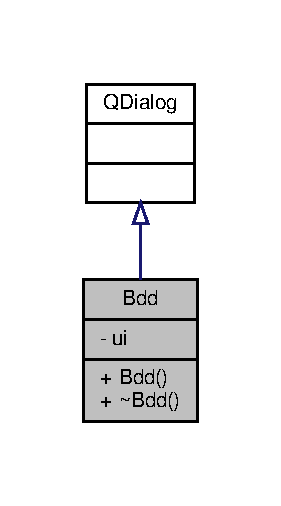
\includegraphics[width=135pt]{class_bdd__coll__graph}
\end{center}
\end{figure}
\subsubsection*{Fonctions membres publiques}
\begin{DoxyCompactItemize}
\item 
\hyperlink{class_bdd_a9b439e0eaab93fcea818892e1daf809b}{Bdd} (\hyperlink{class_q_widget}{Q\+Widget} $\ast$parent=nullptr)
\item 
\hyperlink{class_bdd_a5029277f27f8cfcf9d8603fb331a15dd}{$\sim$\+Bdd} ()
\end{DoxyCompactItemize}
\subsubsection*{Attributs privés}
\begin{DoxyCompactItemize}
\item 
Ui\+::\+Bdd $\ast$ \hyperlink{class_bdd_a7d9f43a44caaddb2f5ccd728ecc78c2a}{ui}
\end{DoxyCompactItemize}


\subsubsection{Description détaillée}


Définition à la ligne \hyperlink{bdd_8h_source_l00010}{10} du fichier \hyperlink{bdd_8h_source}{bdd.\+h}.



\subsubsection{Documentation des constructeurs et destructeur}
\mbox{\Hypertarget{class_bdd_a9b439e0eaab93fcea818892e1daf809b}\label{class_bdd_a9b439e0eaab93fcea818892e1daf809b}} 
\index{Bdd@{Bdd}!Bdd@{Bdd}}
\index{Bdd@{Bdd}!Bdd@{Bdd}}
\paragraph{\texorpdfstring{Bdd()}{Bdd()}}
{\footnotesize\ttfamily Bdd\+::\+Bdd (\begin{DoxyParamCaption}\item[{\hyperlink{class_q_widget}{Q\+Widget} $\ast$}]{parent = {\ttfamily nullptr} }\end{DoxyParamCaption})\hspace{0.3cm}{\ttfamily [explicit]}}



Définition à la ligne \hyperlink{bdd_8cpp_source_l00004}{4} du fichier \hyperlink{bdd_8cpp_source}{bdd.\+cpp}.



Références \hyperlink{bdd_8h_source_l00019}{ui}.


\begin{DoxyCode}
00004                         :
00005     \hyperlink{class_q_dialog}{QDialog}(parent),
00006     \hyperlink{class_bdd_a7d9f43a44caaddb2f5ccd728ecc78c2a}{ui}(\textcolor{keyword}{new} Ui::Bdd)
00007 \{
00008     \hyperlink{class_bdd_a7d9f43a44caaddb2f5ccd728ecc78c2a}{ui}->setupUi(\textcolor{keyword}{this});
00009 \}
\end{DoxyCode}
\mbox{\Hypertarget{class_bdd_a5029277f27f8cfcf9d8603fb331a15dd}\label{class_bdd_a5029277f27f8cfcf9d8603fb331a15dd}} 
\index{Bdd@{Bdd}!````~Bdd@{$\sim$\+Bdd}}
\index{````~Bdd@{$\sim$\+Bdd}!Bdd@{Bdd}}
\paragraph{\texorpdfstring{$\sim$\+Bdd()}{~Bdd()}}
{\footnotesize\ttfamily Bdd\+::$\sim$\+Bdd (\begin{DoxyParamCaption}{ }\end{DoxyParamCaption})}



Définition à la ligne \hyperlink{bdd_8cpp_source_l00011}{11} du fichier \hyperlink{bdd_8cpp_source}{bdd.\+cpp}.



Références \hyperlink{bdd_8h_source_l00019}{ui}.


\begin{DoxyCode}
00012 \{
00013     \textcolor{keyword}{delete} \hyperlink{class_bdd_a7d9f43a44caaddb2f5ccd728ecc78c2a}{ui};
00014 \}
\end{DoxyCode}


\subsubsection{Documentation des données membres}
\mbox{\Hypertarget{class_bdd_a7d9f43a44caaddb2f5ccd728ecc78c2a}\label{class_bdd_a7d9f43a44caaddb2f5ccd728ecc78c2a}} 
\index{Bdd@{Bdd}!ui@{ui}}
\index{ui@{ui}!Bdd@{Bdd}}
\paragraph{\texorpdfstring{ui}{ui}}
{\footnotesize\ttfamily Ui\+::\+Bdd$\ast$ Bdd\+::ui\hspace{0.3cm}{\ttfamily [private]}}



Définition à la ligne \hyperlink{bdd_8h_source_l00019}{19} du fichier \hyperlink{bdd_8h_source}{bdd.\+h}.



Référencé par \hyperlink{bdd_8cpp_source_l00004}{Bdd()}, et \hyperlink{bdd_8cpp_source_l00011}{$\sim$\+Bdd()}.



La documentation de cette classe a été générée à partir des fichiers suivants \+:\begin{DoxyCompactItemize}
\item 
\hyperlink{bdd_8h}{bdd.\+h}\item 
\hyperlink{bdd_8cpp}{bdd.\+cpp}\end{DoxyCompactItemize}

\hypertarget{class_communication_bluetooth}{}\subsection{Référence de la classe Communication\+Bluetooth}
\label{class_communication_bluetooth}\index{Communication\+Bluetooth@{Communication\+Bluetooth}}


Class permettant de mettre en place une communication bluetooth.  




{\ttfamily \#include \char`\"{}communicationbluetooth.\+h\char`\"{}}



Graphe de collaboration de Communication\+Bluetooth\+:
\nopagebreak
\begin{figure}[H]
\begin{center}
\leavevmode
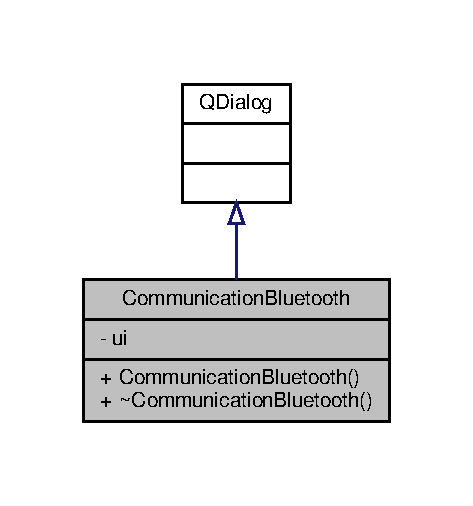
\includegraphics[width=227pt]{class_communication_bluetooth__coll__graph}
\end{center}
\end{figure}
\subsubsection*{Fonctions membres publiques}
\begin{DoxyCompactItemize}
\item 
\hyperlink{class_communication_bluetooth_a30f88d1710eb41d9c8c4b390b5c7b6f7}{Communication\+Bluetooth} (\hyperlink{class_q_widget}{Q\+Widget} $\ast$parent=nullptr)
\begin{DoxyCompactList}\small\item\em Constructeur classe \hyperlink{class_communication_bluetooth}{Communication\+Bluetooth}. \end{DoxyCompactList}\item 
\hyperlink{class_communication_bluetooth_a13c72d24359f40c204e94f3ef1ab6fd3}{$\sim$\+Communication\+Bluetooth} ()
\begin{DoxyCompactList}\small\item\em Destructeur classe \hyperlink{class_communication_bluetooth}{Communication\+Bluetooth}. \end{DoxyCompactList}\end{DoxyCompactItemize}
\subsubsection*{Attributs privés}
\begin{DoxyCompactItemize}
\item 
Ui\+::\+Communication\+Bluetooth $\ast$ \hyperlink{class_communication_bluetooth_a2721cf9f9503a98770981ffdad09f9a1}{ui}
\end{DoxyCompactItemize}


\subsubsection{Description détaillée}
Class permettant de mettre en place une communication bluetooth. 

Définition à la ligne \hyperlink{communicationbluetooth_8h_source_l00017}{17} du fichier \hyperlink{communicationbluetooth_8h_source}{communicationbluetooth.\+h}.



\subsubsection{Documentation des constructeurs et destructeur}
\mbox{\Hypertarget{class_communication_bluetooth_a30f88d1710eb41d9c8c4b390b5c7b6f7}\label{class_communication_bluetooth_a30f88d1710eb41d9c8c4b390b5c7b6f7}} 
\index{Communication\+Bluetooth@{Communication\+Bluetooth}!Communication\+Bluetooth@{Communication\+Bluetooth}}
\index{Communication\+Bluetooth@{Communication\+Bluetooth}!Communication\+Bluetooth@{Communication\+Bluetooth}}
\paragraph{\texorpdfstring{Communication\+Bluetooth()}{CommunicationBluetooth()}}
{\footnotesize\ttfamily Communication\+Bluetooth\+::\+Communication\+Bluetooth (\begin{DoxyParamCaption}\item[{\hyperlink{class_q_widget}{Q\+Widget} $\ast$}]{parent = {\ttfamily nullptr} }\end{DoxyParamCaption})\hspace{0.3cm}{\ttfamily [explicit]}}



Constructeur classe \hyperlink{class_communication_bluetooth}{Communication\+Bluetooth}. 


\begin{DoxyParams}{Paramètres}
{\em parent} & \\
\hline
\end{DoxyParams}


Définition à la ligne \hyperlink{communicationbluetooth_8cpp_source_l00004}{4} du fichier \hyperlink{communicationbluetooth_8cpp_source}{communicationbluetooth.\+cpp}.



Références \hyperlink{communicationbluetooth_8h_source_l00038}{ui}.


\begin{DoxyCode}
00004                                                               :
00005     \hyperlink{class_q_dialog}{QDialog}(parent),
00006     \hyperlink{class_communication_bluetooth_a2721cf9f9503a98770981ffdad09f9a1}{ui}(\textcolor{keyword}{new} Ui::CommunicationBluetooth)
00007 \{
00008      qDebug() << Q\_FUNC\_INFO;
00009     \hyperlink{class_communication_bluetooth_a2721cf9f9503a98770981ffdad09f9a1}{ui}->setupUi(\textcolor{keyword}{this});
00010 \}
\end{DoxyCode}
\mbox{\Hypertarget{class_communication_bluetooth_a13c72d24359f40c204e94f3ef1ab6fd3}\label{class_communication_bluetooth_a13c72d24359f40c204e94f3ef1ab6fd3}} 
\index{Communication\+Bluetooth@{Communication\+Bluetooth}!````~Communication\+Bluetooth@{$\sim$\+Communication\+Bluetooth}}
\index{````~Communication\+Bluetooth@{$\sim$\+Communication\+Bluetooth}!Communication\+Bluetooth@{Communication\+Bluetooth}}
\paragraph{\texorpdfstring{$\sim$\+Communication\+Bluetooth()}{~CommunicationBluetooth()}}
{\footnotesize\ttfamily Communication\+Bluetooth\+::$\sim$\+Communication\+Bluetooth (\begin{DoxyParamCaption}{ }\end{DoxyParamCaption})}



Destructeur classe \hyperlink{class_communication_bluetooth}{Communication\+Bluetooth}. 


\begin{DoxyParams}{Paramètres}
{\em parent} & \\
\hline
\end{DoxyParams}


Définition à la ligne \hyperlink{communicationbluetooth_8cpp_source_l00012}{12} du fichier \hyperlink{communicationbluetooth_8cpp_source}{communicationbluetooth.\+cpp}.



Références \hyperlink{communicationbluetooth_8h_source_l00038}{ui}.


\begin{DoxyCode}
00013 \{
00014     \textcolor{keyword}{delete} \hyperlink{class_communication_bluetooth_a2721cf9f9503a98770981ffdad09f9a1}{ui};
00015     qDebug() << Q\_FUNC\_INFO;
00016 \}
\end{DoxyCode}


\subsubsection{Documentation des données membres}
\mbox{\Hypertarget{class_communication_bluetooth_a2721cf9f9503a98770981ffdad09f9a1}\label{class_communication_bluetooth_a2721cf9f9503a98770981ffdad09f9a1}} 
\index{Communication\+Bluetooth@{Communication\+Bluetooth}!ui@{ui}}
\index{ui@{ui}!Communication\+Bluetooth@{Communication\+Bluetooth}}
\paragraph{\texorpdfstring{ui}{ui}}
{\footnotesize\ttfamily Ui\+::\+Communication\+Bluetooth$\ast$ Communication\+Bluetooth\+::ui\hspace{0.3cm}{\ttfamily [private]}}



Définition à la ligne \hyperlink{communicationbluetooth_8h_source_l00038}{38} du fichier \hyperlink{communicationbluetooth_8h_source}{communicationbluetooth.\+h}.



Référencé par \hyperlink{communicationbluetooth_8cpp_source_l00004}{Communication\+Bluetooth()}, et \hyperlink{communicationbluetooth_8cpp_source_l00012}{$\sim$\+Communication\+Bluetooth()}.



La documentation de cette classe a été générée à partir des fichiers suivants \+:\begin{DoxyCompactItemize}
\item 
\hyperlink{communicationbluetooth_8h}{communicationbluetooth.\+h}\item 
\hyperlink{communicationbluetooth_8cpp}{communicationbluetooth.\+cpp}\end{DoxyCompactItemize}

\hypertarget{class_controle}{}\subsection{Référence de la classe Controle}
\label{class_controle}\index{Controle@{Controle}}


Classe assurant le controle et la validé de l\textquotesingle{}envoie et réception des trames.  




{\ttfamily \#include \char`\"{}controle.\+h\char`\"{}}



Graphe de collaboration de Controle\+:
\nopagebreak
\begin{figure}[H]
\begin{center}
\leavevmode
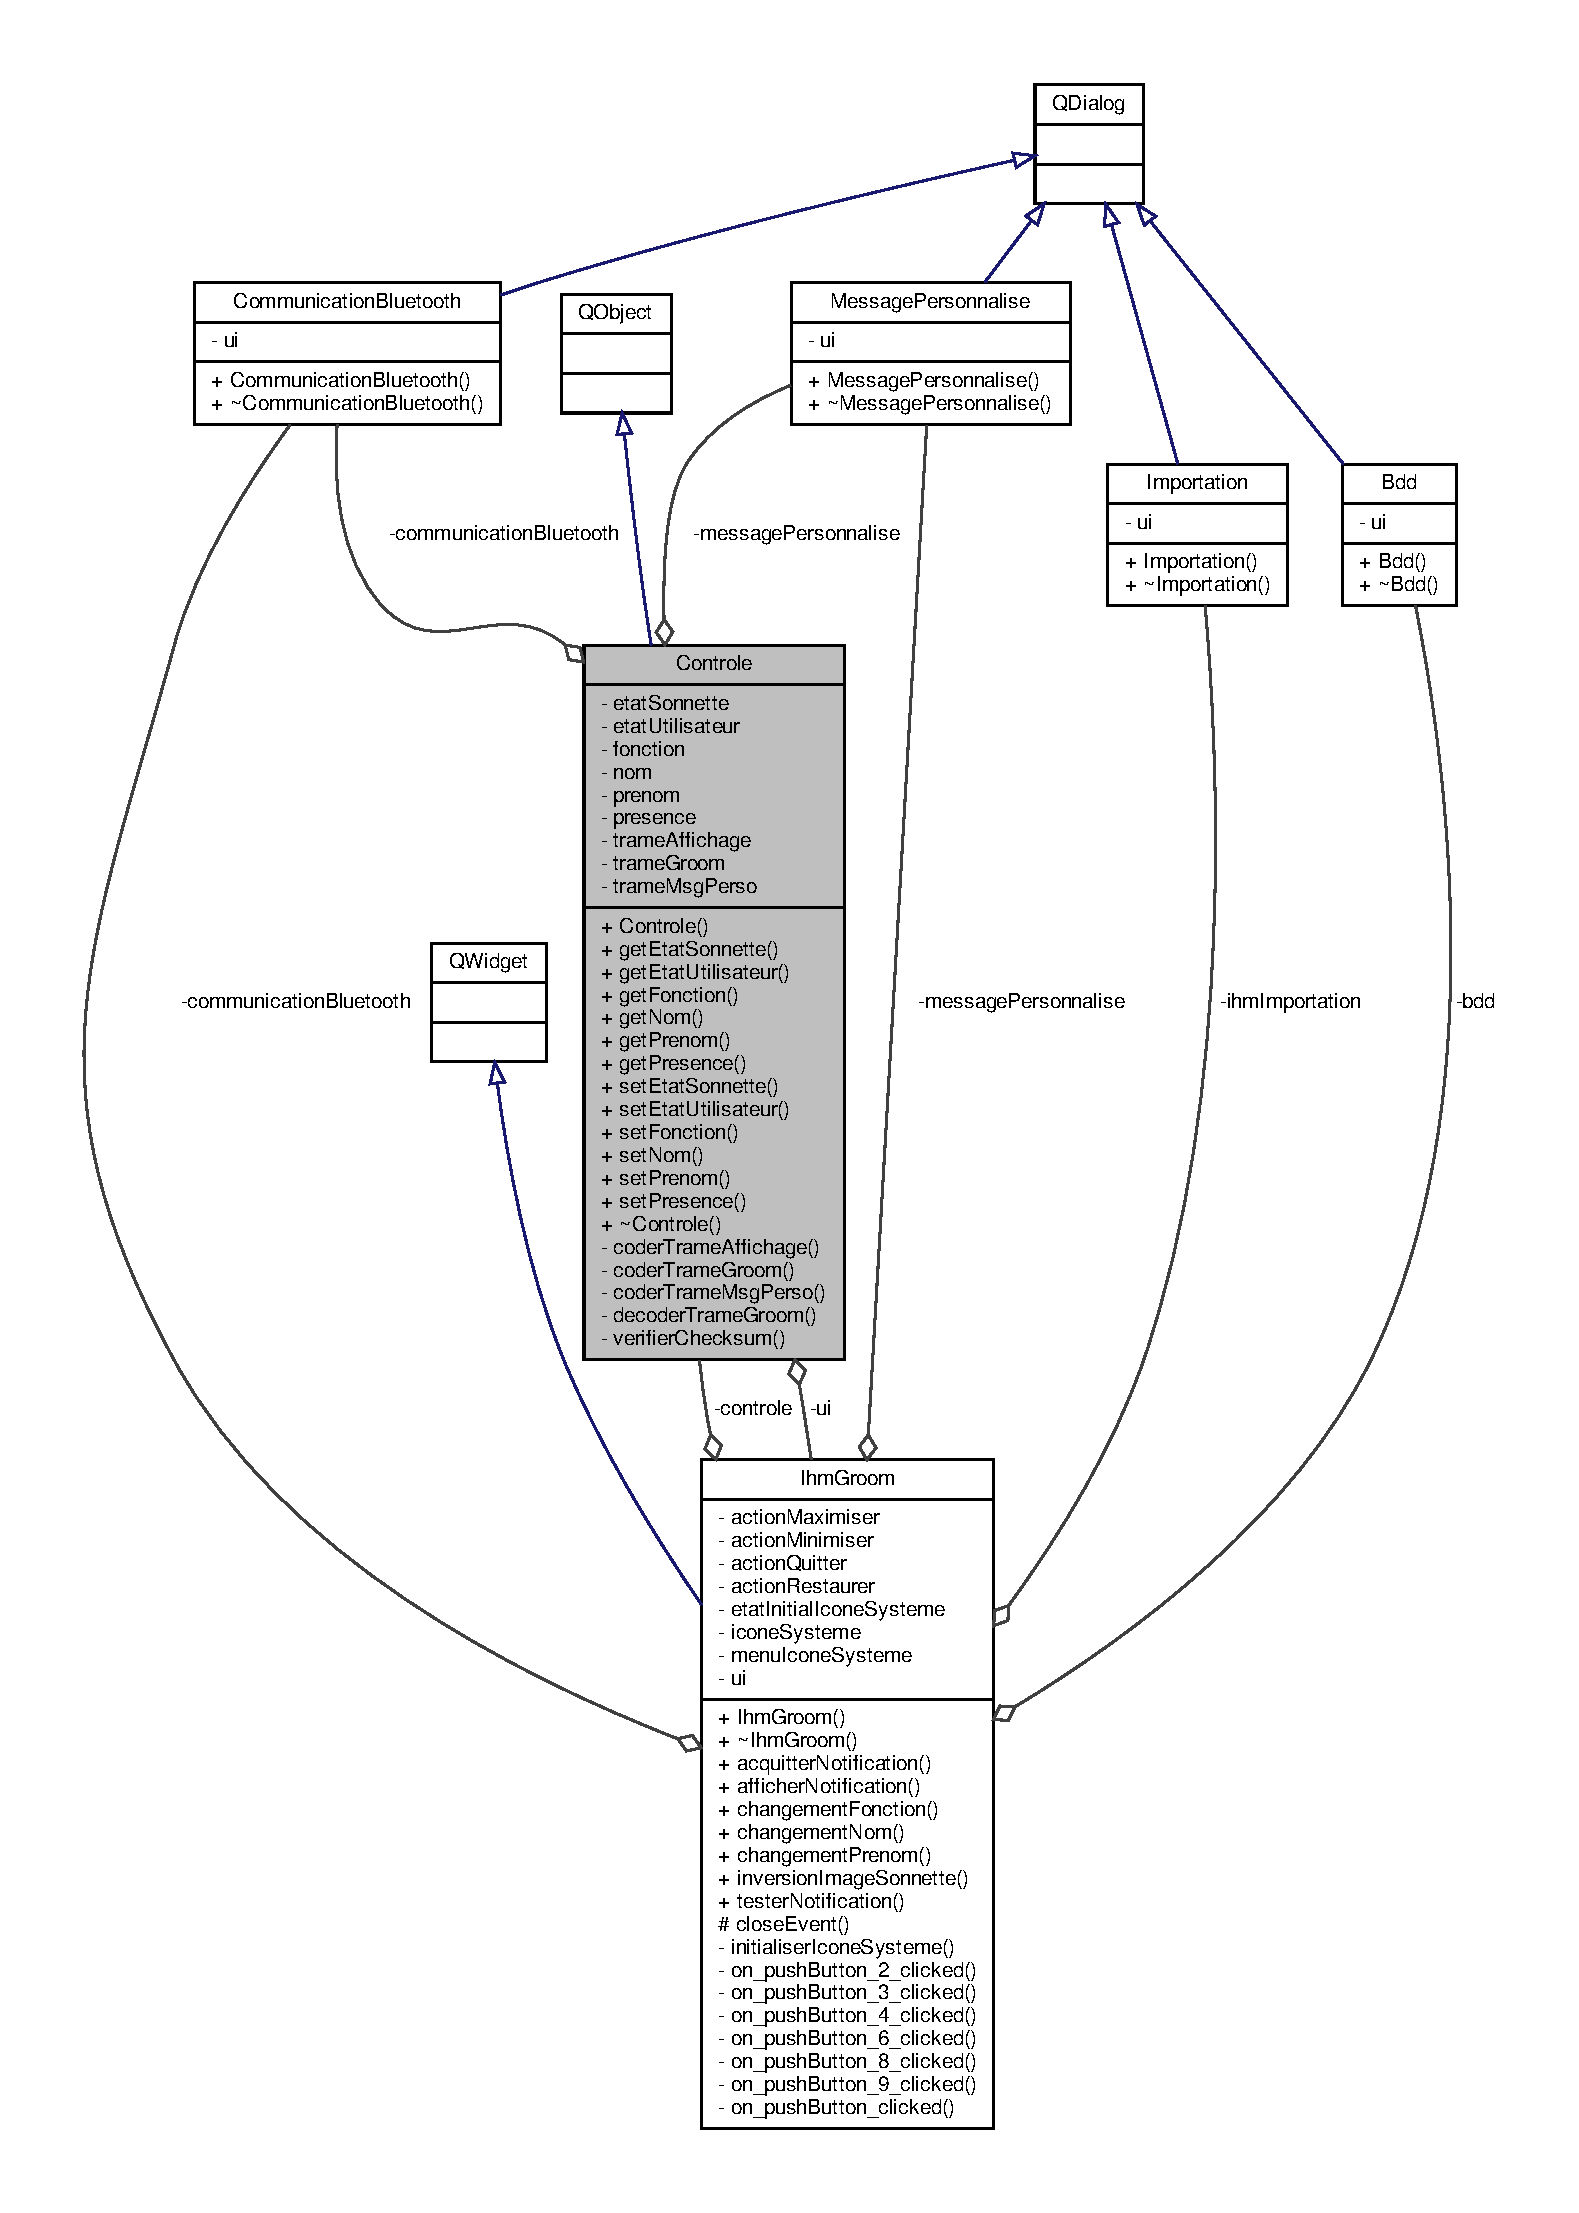
\includegraphics[width=350pt]{class_controle__coll__graph}
\end{center}
\end{figure}
\subsubsection*{Fonctions membres publiques}
\begin{DoxyCompactItemize}
\item 
\hyperlink{class_controle_af64a33acc664bf02f2ea0b4f27f781e6}{Controle} (\hyperlink{class_q_object}{Q\+Object} $\ast$parent=nullptr)
\begin{DoxyCompactList}\small\item\em Constructeur classe \hyperlink{class_controle}{Controle}. \end{DoxyCompactList}\item 
bool \hyperlink{class_controle_acabf3768430c7f1acb268ca0fa1ddf99}{get\+Etat\+Sonnette} ()
\begin{DoxyCompactList}\small\item\em retroune l\textquotesingle{}état de la sonnette \end{DoxyCompactList}\item 
int \hyperlink{class_controle_ac3bd8e8621cee56d4343e21a624e1c48}{get\+Etat\+Utilisateur} ()
\begin{DoxyCompactList}\small\item\em retroune l\textquotesingle{}état de la sonnette \end{DoxyCompactList}\item 
Q\+String \hyperlink{class_controle_a8d2891b2b01c503d10f775b4b14a3777}{get\+Fonction} ()
\begin{DoxyCompactList}\small\item\em retroune la fonction \end{DoxyCompactList}\item 
Q\+String \hyperlink{class_controle_ac6e8590a5108e97fce3ce3aa43feb881}{get\+Nom} ()
\begin{DoxyCompactList}\small\item\em retroune le nom \end{DoxyCompactList}\item 
Q\+String \hyperlink{class_controle_a0164fd9066b1703498576095ab5642c5}{get\+Prenom} ()
\begin{DoxyCompactList}\small\item\em retroune le prenom \end{DoxyCompactList}\item 
bool \hyperlink{class_controle_abf7c9fefec4980b90c9f759d48fd17aa}{get\+Presence} ()
\begin{DoxyCompactList}\small\item\em retroune l\textquotesingle{}état de la sonnette \end{DoxyCompactList}\item 
void \hyperlink{class_controle_ac706c5e9ede46dab70631281b084e233}{set\+Etat\+Sonnette} (bool new\+Etat\+Sonnette)
\begin{DoxyCompactList}\small\item\em modifie l\textquotesingle{}état de la sonnette \end{DoxyCompactList}\item 
void \hyperlink{class_controle_a62db54114d126d03dd332332b3942320}{set\+Etat\+Utilisateur} (int new\+Etat\+Utilisateur)
\begin{DoxyCompactList}\small\item\em modifie l\textquotesingle{}état de la sonnette \end{DoxyCompactList}\item 
void \hyperlink{class_controle_abe472f4fd197c0fc679539e0b75a6e15}{set\+Fonction} (Q\+String new\+Fonction)
\begin{DoxyCompactList}\small\item\em modifie la fonction \end{DoxyCompactList}\item 
void \hyperlink{class_controle_a0f731cdb733053f7be24e7042611601c}{set\+Nom} (Q\+String new\+Nom)
\begin{DoxyCompactList}\small\item\em modifie le nom \end{DoxyCompactList}\item 
void \hyperlink{class_controle_ab046adc050872b4034c1500eb2e1b728}{set\+Prenom} (Q\+String new\+Prenom)
\item 
void \hyperlink{class_controle_a65904fe693663759a4cde4e4d66e36e8}{set\+Presence} (bool new\+Presence)
\begin{DoxyCompactList}\small\item\em modifie l\textquotesingle{}état de la présence \end{DoxyCompactList}\item 
\hyperlink{class_controle_a98f5d2630efbdb5f469cbb2675725b20}{$\sim$\+Controle} ()
\begin{DoxyCompactList}\small\item\em Destructeur classe \hyperlink{class_controle}{Controle}. \end{DoxyCompactList}\end{DoxyCompactItemize}
\subsubsection*{Fonctions membres privées}
\begin{DoxyCompactItemize}
\item 
void \hyperlink{class_controle_a316808279226b01ac8fe51ab396b1b67}{coder\+Trame\+Affichage} (Q\+String \hyperlink{class_controle_a0bbdd7a0c44fbbc45bf3a381872fcfbe}{trame\+Affichage})
\begin{DoxyCompactList}\small\item\em coder la trame Affichage \end{DoxyCompactList}\item 
void \hyperlink{class_controle_a9ba8efd42493ffd4288537a1ace4e220}{coder\+Trame\+Groom} (Q\+String \hyperlink{class_controle_a5b9512ebbaf16746f55a9519de88f9be}{trame\+Groom})
\begin{DoxyCompactList}\small\item\em coder la trame Groom \end{DoxyCompactList}\item 
void \hyperlink{class_controle_a77d635484c2e6fca851d40e76f422fce}{coder\+Trame\+Msg\+Perso} (Q\+String \hyperlink{class_controle_a5cb6dbeb8b2f066b1e757f3c933ea503}{trame\+Msg\+Perso})
\begin{DoxyCompactList}\small\item\em coder la trame Msg Perso \end{DoxyCompactList}\item 
void \hyperlink{class_controle_a2dcdd01e67e6ce8769188d62ce0c262a}{decoder\+Trame\+Groom} (Q\+String \hyperlink{class_controle_a5b9512ebbaf16746f55a9519de88f9be}{trame\+Groom})
\begin{DoxyCompactList}\small\item\em Décode la trame Groom. \end{DoxyCompactList}\item 
bool \hyperlink{class_controle_a4f40023a18e4e656282a15d5657e0a25}{verifier\+Checksum} (Q\+String \hyperlink{class_controle_a5b9512ebbaf16746f55a9519de88f9be}{trame\+Groom})
\begin{DoxyCompactList}\small\item\em Regarde le checksum de la trame\+Groom. \end{DoxyCompactList}\end{DoxyCompactItemize}
\subsubsection*{Attributs privés}
\begin{DoxyCompactItemize}
\item 
\hyperlink{class_communication_bluetooth}{Communication\+Bluetooth} $\ast$ \hyperlink{class_controle_a5d818564000173732472eb9ac20e53aa}{communication\+Bluetooth}
\item 
bool \hyperlink{class_controle_afddf1dce812ff88577e308684b564f33}{etat\+Sonnette}
\item 
int \hyperlink{class_controle_a690595803de8f5c172b8bc46122ebb1a}{etat\+Utilisateur}
\item 
Q\+String \hyperlink{class_controle_af733c06309ce63fb9157073574e42b00}{fonction}
\item 
\hyperlink{class_message_personnalise}{Message\+Personnalise} $\ast$ \hyperlink{class_controle_a6240fc19c937146243bcd950e5408481}{message\+Personnalise}
\item 
Q\+String \hyperlink{class_controle_ad47747a49ca21434f6d43d451d3cf134}{nom}
\item 
Q\+String \hyperlink{class_controle_a29e37e25a6fd4643ddea3fef47e3bc51}{prenom}
\item 
bool \hyperlink{class_controle_a089f74f48f24f09e7fc51b03a5ede79e}{presence}
\item 
Q\+String \hyperlink{class_controle_a0bbdd7a0c44fbbc45bf3a381872fcfbe}{trame\+Affichage}
\item 
Q\+String \hyperlink{class_controle_a5b9512ebbaf16746f55a9519de88f9be}{trame\+Groom}
\item 
Q\+String \hyperlink{class_controle_a5cb6dbeb8b2f066b1e757f3c933ea503}{trame\+Msg\+Perso}
\item 
\hyperlink{class_ihm_groom}{Ihm\+Groom} $\ast$ \hyperlink{class_controle_a2dd60c955396dd80426c1a74f56ea611}{ui}
\end{DoxyCompactItemize}


\subsubsection{Description détaillée}
Classe assurant le controle et la validé de l\textquotesingle{}envoie et réception des trames. 

Définition à la ligne \hyperlink{controle_8h_source_l00022}{22} du fichier \hyperlink{controle_8h_source}{controle.\+h}.



\subsubsection{Documentation des constructeurs et destructeur}
\mbox{\Hypertarget{class_controle_af64a33acc664bf02f2ea0b4f27f781e6}\label{class_controle_af64a33acc664bf02f2ea0b4f27f781e6}} 
\index{Controle@{Controle}!Controle@{Controle}}
\index{Controle@{Controle}!Controle@{Controle}}
\paragraph{\texorpdfstring{Controle()}{Controle()}}
{\footnotesize\ttfamily Controle\+::\+Controle (\begin{DoxyParamCaption}\item[{\hyperlink{class_q_object}{Q\+Object} $\ast$}]{parent = {\ttfamily nullptr} }\end{DoxyParamCaption})}



Constructeur classe \hyperlink{class_controle}{Controle}. 

Attribut de la fonction de l\textquotesingle{}utilisateur 
\begin{DoxyParams}{Paramètres}
{\em parent} & \\
\hline
\end{DoxyParams}


Définition à la ligne \hyperlink{controle_8cpp_source_l00005}{5} du fichier \hyperlink{controle_8cpp_source}{controle.\+cpp}.



Références \hyperlink{controle_8h_source_l00070}{etat\+Sonnette}.


\begin{DoxyCode}
00005                                   : \hyperlink{class_q_object}{QObject}(parent)
00006 \{
00007      qDebug() << Q\_FUNC\_INFO;
00008    \textcolor{comment}{//     ui = new IhmGroom;}
00009     \hyperlink{class_controle_afddf1dce812ff88577e308684b564f33}{etatSonnette} = \textcolor{keyword}{true};
00010 
00011 \}
\end{DoxyCode}
\mbox{\Hypertarget{class_controle_a98f5d2630efbdb5f469cbb2675725b20}\label{class_controle_a98f5d2630efbdb5f469cbb2675725b20}} 
\index{Controle@{Controle}!````~Controle@{$\sim$\+Controle}}
\index{````~Controle@{$\sim$\+Controle}!Controle@{Controle}}
\paragraph{\texorpdfstring{$\sim$\+Controle()}{~Controle()}}
{\footnotesize\ttfamily Controle\+::$\sim$\+Controle (\begin{DoxyParamCaption}{ }\end{DoxyParamCaption})}



Destructeur classe \hyperlink{class_controle}{Controle}. 


\begin{DoxyParams}{Paramètres}
{\em parent} & \\
\hline
\end{DoxyParams}


Définition à la ligne \hyperlink{controle_8cpp_source_l00013}{13} du fichier \hyperlink{controle_8cpp_source}{controle.\+cpp}.


\begin{DoxyCode}
00014 \{
00015     qDebug() << Q\_FUNC\_INFO;
00016 \}
\end{DoxyCode}


\subsubsection{Documentation des fonctions membres}
\mbox{\Hypertarget{class_controle_a316808279226b01ac8fe51ab396b1b67}\label{class_controle_a316808279226b01ac8fe51ab396b1b67}} 
\index{Controle@{Controle}!coder\+Trame\+Affichage@{coder\+Trame\+Affichage}}
\index{coder\+Trame\+Affichage@{coder\+Trame\+Affichage}!Controle@{Controle}}
\paragraph{\texorpdfstring{coder\+Trame\+Affichage()}{coderTrameAffichage()}}
{\footnotesize\ttfamily Controle\+::coder\+Trame\+Affichage (\begin{DoxyParamCaption}\item[{Q\+String}]{trame\+Affichage }\end{DoxyParamCaption})\hspace{0.3cm}{\ttfamily [private]}}



coder la trame Affichage 



Définition à la ligne \hyperlink{controle_8cpp_source_l00101}{101} du fichier \hyperlink{controle_8cpp_source}{controle.\+cpp}.



Références \hyperlink{ihmgroom_8cpp_source_l00075}{Ihm\+Groom\+::changement\+Fonction()}, \hyperlink{ihmgroom_8cpp_source_l00065}{Ihm\+Groom\+::changement\+Nom()}, \hyperlink{ihmgroom_8cpp_source_l00070}{Ihm\+Groom\+::changement\+Prenom()}, \hyperlink{controle_8cpp_source_l00092}{set\+Fonction()}, \hyperlink{controle_8cpp_source_l00075}{set\+Nom()}, \hyperlink{controle_8cpp_source_l00084}{set\+Prenom()}, et \hyperlink{controle_8h_source_l00029}{ui}.


\begin{DoxyCode}
00102 \{
00103     \hyperlink{class_controle_a0f731cdb733053f7be24e7042611601c}{setNom}(\hyperlink{class_controle_a0bbdd7a0c44fbbc45bf3a381872fcfbe}{trameAffichage}.section(\textcolor{stringliteral}{";"},1,1));
00104 
00105     \hyperlink{class_controle_ab046adc050872b4034c1500eb2e1b728}{setPrenom}(\hyperlink{class_controle_a0bbdd7a0c44fbbc45bf3a381872fcfbe}{trameAffichage}.section(\textcolor{stringliteral}{";"},2,2));
00106 
00107     \hyperlink{class_controle_abe472f4fd197c0fc679539e0b75a6e15}{setFonction}(\hyperlink{class_controle_a0bbdd7a0c44fbbc45bf3a381872fcfbe}{trameAffichage}.section(\textcolor{stringliteral}{";"},3,3));
00108 
00109     \hyperlink{class_controle_a2dd60c955396dd80426c1a74f56ea611}{ui}->\hyperlink{class_ihm_groom_aa270d1fb6a7a9c1385c4ae3e67451ea0}{changementNom}();
00110     \hyperlink{class_controle_a2dd60c955396dd80426c1a74f56ea611}{ui}->\hyperlink{class_ihm_groom_a2e8db190224f15326552a5bd642a9347}{changementPrenom}();
00111     \hyperlink{class_controle_a2dd60c955396dd80426c1a74f56ea611}{ui}->\hyperlink{class_ihm_groom_afc6c48489b270b22a660e32668d6b2ca}{changementFonction}();
00112 \}
\end{DoxyCode}
\mbox{\Hypertarget{class_controle_a9ba8efd42493ffd4288537a1ace4e220}\label{class_controle_a9ba8efd42493ffd4288537a1ace4e220}} 
\index{Controle@{Controle}!coder\+Trame\+Groom@{coder\+Trame\+Groom}}
\index{coder\+Trame\+Groom@{coder\+Trame\+Groom}!Controle@{Controle}}
\paragraph{\texorpdfstring{coder\+Trame\+Groom()}{coderTrameGroom()}}
{\footnotesize\ttfamily Controle\+::coder\+Trame\+Groom (\begin{DoxyParamCaption}\item[{Q\+String}]{trame\+Groom }\end{DoxyParamCaption})\hspace{0.3cm}{\ttfamily [private]}}



coder la trame Groom 

\mbox{\Hypertarget{class_controle_a77d635484c2e6fca851d40e76f422fce}\label{class_controle_a77d635484c2e6fca851d40e76f422fce}} 
\index{Controle@{Controle}!coder\+Trame\+Msg\+Perso@{coder\+Trame\+Msg\+Perso}}
\index{coder\+Trame\+Msg\+Perso@{coder\+Trame\+Msg\+Perso}!Controle@{Controle}}
\paragraph{\texorpdfstring{coder\+Trame\+Msg\+Perso()}{coderTrameMsgPerso()}}
{\footnotesize\ttfamily Controle\+::coder\+Trame\+Msg\+Perso (\begin{DoxyParamCaption}\item[{Q\+String}]{trame\+Msg\+Perso }\end{DoxyParamCaption})\hspace{0.3cm}{\ttfamily [private]}}



coder la trame Msg Perso 

\mbox{\Hypertarget{class_controle_a2dcdd01e67e6ce8769188d62ce0c262a}\label{class_controle_a2dcdd01e67e6ce8769188d62ce0c262a}} 
\index{Controle@{Controle}!decoder\+Trame\+Groom@{decoder\+Trame\+Groom}}
\index{decoder\+Trame\+Groom@{decoder\+Trame\+Groom}!Controle@{Controle}}
\paragraph{\texorpdfstring{decoder\+Trame\+Groom()}{decoderTrameGroom()}}
{\footnotesize\ttfamily Controle\+::decoder\+Trame\+Groom (\begin{DoxyParamCaption}\item[{Q\+String}]{trame\+Groom }\end{DoxyParamCaption})\hspace{0.3cm}{\ttfamily [private]}}



Décode la trame Groom. 



Définition à la ligne \hyperlink{controle_8cpp_source_l00049}{49} du fichier \hyperlink{controle_8cpp_source}{controle.\+cpp}.



Références \hyperlink{controle_8cpp_source_l00028}{set\+Etat\+Sonnette()}, \hyperlink{controle_8cpp_source_l00018}{set\+Etat\+Utilisateur()}, et \hyperlink{controle_8cpp_source_l00038}{set\+Presence()}.


\begin{DoxyCode}
00050 \{
00051 
00052     \hyperlink{class_controle_a62db54114d126d03dd332332b3942320}{setEtatUtilisateur}((\hyperlink{class_controle_a5b9512ebbaf16746f55a9519de88f9be}{trameGroom}.section(\textcolor{stringliteral}{";"},1,1)).toInt());
00053 
00054 
00055     \textcolor{keywordflow}{if} (\hyperlink{class_controle_a5b9512ebbaf16746f55a9519de88f9be}{trameGroom}.section(\textcolor{stringliteral}{";"},2,2) == 1)
00056     \{
00057         \hyperlink{class_controle_ac706c5e9ede46dab70631281b084e233}{setEtatSonnette}(\textcolor{keyword}{true});
00058     \}
00059     \textcolor{keywordflow}{else}
00060     \{
00061         \hyperlink{class_controle_ac706c5e9ede46dab70631281b084e233}{setEtatSonnette}(\textcolor{keyword}{false});
00062     \}
00063 
00064     \textcolor{keywordflow}{if} (\hyperlink{class_controle_a5b9512ebbaf16746f55a9519de88f9be}{trameGroom}.section(\textcolor{stringliteral}{";"},3,3) == 1)
00065     \{
00066         \hyperlink{class_controle_a65904fe693663759a4cde4e4d66e36e8}{setPresence}(\textcolor{keyword}{true});
00067     \}
00068     \textcolor{keywordflow}{else}
00069     \{
00070         \hyperlink{class_controle_a65904fe693663759a4cde4e4d66e36e8}{setPresence}(\textcolor{keyword}{false});
00071     \}
00072 
00073 \}
\end{DoxyCode}
\mbox{\Hypertarget{class_controle_acabf3768430c7f1acb268ca0fa1ddf99}\label{class_controle_acabf3768430c7f1acb268ca0fa1ddf99}} 
\index{Controle@{Controle}!get\+Etat\+Sonnette@{get\+Etat\+Sonnette}}
\index{get\+Etat\+Sonnette@{get\+Etat\+Sonnette}!Controle@{Controle}}
\paragraph{\texorpdfstring{get\+Etat\+Sonnette()}{getEtatSonnette()}}
{\footnotesize\ttfamily Controle\+::get\+Etat\+Sonnette (\begin{DoxyParamCaption}{ }\end{DoxyParamCaption})}



retroune l\textquotesingle{}état de la sonnette 

\begin{DoxyReturn}{Renvoie}
etat\+Sonnette 
\end{DoxyReturn}


Définition à la ligne \hyperlink{controle_8cpp_source_l00033}{33} du fichier \hyperlink{controle_8cpp_source}{controle.\+cpp}.



Références \hyperlink{controle_8h_source_l00070}{etat\+Sonnette}.



Référencé par \hyperlink{ihmgroom_8cpp_source_l00201}{Ihm\+Groom\+::inversion\+Image\+Sonnette()}.


\begin{DoxyCode}
00034 \{
00035     \textcolor{keywordflow}{return} \hyperlink{class_controle_afddf1dce812ff88577e308684b564f33}{etatSonnette};
00036 \}
\end{DoxyCode}
\mbox{\Hypertarget{class_controle_ac3bd8e8621cee56d4343e21a624e1c48}\label{class_controle_ac3bd8e8621cee56d4343e21a624e1c48}} 
\index{Controle@{Controle}!get\+Etat\+Utilisateur@{get\+Etat\+Utilisateur}}
\index{get\+Etat\+Utilisateur@{get\+Etat\+Utilisateur}!Controle@{Controle}}
\paragraph{\texorpdfstring{get\+Etat\+Utilisateur()}{getEtatUtilisateur()}}
{\footnotesize\ttfamily Controle\+::get\+Etat\+Utilisateur (\begin{DoxyParamCaption}{ }\end{DoxyParamCaption})}



retroune l\textquotesingle{}état de la sonnette 

\begin{DoxyReturn}{Renvoie}
etat\+Utilisateur 
\end{DoxyReturn}


Définition à la ligne \hyperlink{controle_8cpp_source_l00023}{23} du fichier \hyperlink{controle_8cpp_source}{controle.\+cpp}.



Références \hyperlink{controle_8h_source_l00069}{etat\+Utilisateur}.


\begin{DoxyCode}
00024 \{
00025     \textcolor{keywordflow}{return} \hyperlink{class_controle_a690595803de8f5c172b8bc46122ebb1a}{etatUtilisateur};
00026 \}
\end{DoxyCode}
\mbox{\Hypertarget{class_controle_a8d2891b2b01c503d10f775b4b14a3777}\label{class_controle_a8d2891b2b01c503d10f775b4b14a3777}} 
\index{Controle@{Controle}!get\+Fonction@{get\+Fonction}}
\index{get\+Fonction@{get\+Fonction}!Controle@{Controle}}
\paragraph{\texorpdfstring{get\+Fonction()}{getFonction()}}
{\footnotesize\ttfamily Controle\+::get\+Fonction (\begin{DoxyParamCaption}{ }\end{DoxyParamCaption})}



retroune la fonction 

\begin{DoxyReturn}{Renvoie}
fonction 
\end{DoxyReturn}


Définition à la ligne \hyperlink{controle_8cpp_source_l00096}{96} du fichier \hyperlink{controle_8cpp_source}{controle.\+cpp}.



Références \hyperlink{controle_8h_source_l00075}{fonction}.



Référencé par \hyperlink{ihmgroom_8cpp_source_l00075}{Ihm\+Groom\+::changement\+Fonction()}.


\begin{DoxyCode}
00097 \{
00098     \textcolor{keywordflow}{return} \hyperlink{class_controle_af733c06309ce63fb9157073574e42b00}{fonction};
00099 \}
\end{DoxyCode}
\mbox{\Hypertarget{class_controle_ac6e8590a5108e97fce3ce3aa43feb881}\label{class_controle_ac6e8590a5108e97fce3ce3aa43feb881}} 
\index{Controle@{Controle}!get\+Nom@{get\+Nom}}
\index{get\+Nom@{get\+Nom}!Controle@{Controle}}
\paragraph{\texorpdfstring{get\+Nom()}{getNom()}}
{\footnotesize\ttfamily Controle\+::get\+Nom (\begin{DoxyParamCaption}{ }\end{DoxyParamCaption})}



retroune le nom 

\begin{DoxyReturn}{Renvoie}
nom 
\end{DoxyReturn}


Définition à la ligne \hyperlink{controle_8cpp_source_l00080}{80} du fichier \hyperlink{controle_8cpp_source}{controle.\+cpp}.



Références \hyperlink{controle_8h_source_l00073}{nom}.



Référencé par \hyperlink{ihmgroom_8cpp_source_l00065}{Ihm\+Groom\+::changement\+Nom()}.


\begin{DoxyCode}
00081 \{
00082     \textcolor{keywordflow}{return} \hyperlink{class_controle_ad47747a49ca21434f6d43d451d3cf134}{nom};
00083 \}
\end{DoxyCode}
\mbox{\Hypertarget{class_controle_a0164fd9066b1703498576095ab5642c5}\label{class_controle_a0164fd9066b1703498576095ab5642c5}} 
\index{Controle@{Controle}!get\+Prenom@{get\+Prenom}}
\index{get\+Prenom@{get\+Prenom}!Controle@{Controle}}
\paragraph{\texorpdfstring{get\+Prenom()}{getPrenom()}}
{\footnotesize\ttfamily Controle\+::get\+Prenom (\begin{DoxyParamCaption}{ }\end{DoxyParamCaption})}



retroune le prenom 

\begin{DoxyReturn}{Renvoie}
prenom 
\end{DoxyReturn}


Définition à la ligne \hyperlink{controle_8cpp_source_l00088}{88} du fichier \hyperlink{controle_8cpp_source}{controle.\+cpp}.



Références \hyperlink{controle_8h_source_l00074}{prenom}.



Référencé par \hyperlink{ihmgroom_8cpp_source_l00070}{Ihm\+Groom\+::changement\+Prenom()}.


\begin{DoxyCode}
00089 \{
00090     \textcolor{keywordflow}{return} \hyperlink{class_controle_a29e37e25a6fd4643ddea3fef47e3bc51}{prenom};
00091 \}
\end{DoxyCode}
\mbox{\Hypertarget{class_controle_abf7c9fefec4980b90c9f759d48fd17aa}\label{class_controle_abf7c9fefec4980b90c9f759d48fd17aa}} 
\index{Controle@{Controle}!get\+Presence@{get\+Presence}}
\index{get\+Presence@{get\+Presence}!Controle@{Controle}}
\paragraph{\texorpdfstring{get\+Presence()}{getPresence()}}
{\footnotesize\ttfamily Controle\+::get\+Presence (\begin{DoxyParamCaption}{ }\end{DoxyParamCaption})}



retroune l\textquotesingle{}état de la sonnette 

\begin{DoxyReturn}{Renvoie}
presence 
\end{DoxyReturn}


Définition à la ligne \hyperlink{controle_8cpp_source_l00043}{43} du fichier \hyperlink{controle_8cpp_source}{controle.\+cpp}.



Références \hyperlink{controle_8h_source_l00071}{presence}.


\begin{DoxyCode}
00044 \{
00045     \textcolor{keywordflow}{return} \hyperlink{class_controle_a089f74f48f24f09e7fc51b03a5ede79e}{presence};
00046 \}
\end{DoxyCode}
\mbox{\Hypertarget{class_controle_ac706c5e9ede46dab70631281b084e233}\label{class_controle_ac706c5e9ede46dab70631281b084e233}} 
\index{Controle@{Controle}!set\+Etat\+Sonnette@{set\+Etat\+Sonnette}}
\index{set\+Etat\+Sonnette@{set\+Etat\+Sonnette}!Controle@{Controle}}
\paragraph{\texorpdfstring{set\+Etat\+Sonnette()}{setEtatSonnette()}}
{\footnotesize\ttfamily Controle\+::set\+Etat\+Sonnette (\begin{DoxyParamCaption}\item[{bool}]{new\+Etat\+Sonnette }\end{DoxyParamCaption})}



modifie l\textquotesingle{}état de la sonnette 


\begin{DoxyParams}{Paramètres}
{\em etat\+Sonnette} & \\
\hline
\end{DoxyParams}


Définition à la ligne \hyperlink{controle_8cpp_source_l00028}{28} du fichier \hyperlink{controle_8cpp_source}{controle.\+cpp}.



Références \hyperlink{controle_8h_source_l00070}{etat\+Sonnette}.



Référencé par \hyperlink{controle_8cpp_source_l00049}{decoder\+Trame\+Groom()}, et \hyperlink{ihmgroom_8cpp_source_l00201}{Ihm\+Groom\+::inversion\+Image\+Sonnette()}.


\begin{DoxyCode}
00029 \{
00030     \hyperlink{class_controle_afddf1dce812ff88577e308684b564f33}{etatSonnette} = newEtatSonnette;
00031 \}
\end{DoxyCode}
\mbox{\Hypertarget{class_controle_a62db54114d126d03dd332332b3942320}\label{class_controle_a62db54114d126d03dd332332b3942320}} 
\index{Controle@{Controle}!set\+Etat\+Utilisateur@{set\+Etat\+Utilisateur}}
\index{set\+Etat\+Utilisateur@{set\+Etat\+Utilisateur}!Controle@{Controle}}
\paragraph{\texorpdfstring{set\+Etat\+Utilisateur()}{setEtatUtilisateur()}}
{\footnotesize\ttfamily Controle\+::set\+Etat\+Utilisateur (\begin{DoxyParamCaption}\item[{int}]{new\+Etat\+Utilisateur }\end{DoxyParamCaption})}



modifie l\textquotesingle{}état de la sonnette 


\begin{DoxyParams}{Paramètres}
{\em etat\+Utilisateur} & \\
\hline
\end{DoxyParams}


Définition à la ligne \hyperlink{controle_8cpp_source_l00018}{18} du fichier \hyperlink{controle_8cpp_source}{controle.\+cpp}.



Références \hyperlink{controle_8h_source_l00069}{etat\+Utilisateur}.



Référencé par \hyperlink{controle_8cpp_source_l00049}{decoder\+Trame\+Groom()}, \hyperlink{ihmgroom_8cpp_source_l00229}{Ihm\+Groom\+::on\+\_\+push\+Button\+\_\+2\+\_\+clicked()}, \hyperlink{ihmgroom_8cpp_source_l00219}{Ihm\+Groom\+::on\+\_\+push\+Button\+\_\+3\+\_\+clicked()}, et \hyperlink{ihmgroom_8cpp_source_l00224}{Ihm\+Groom\+::on\+\_\+push\+Button\+\_\+4\+\_\+clicked()}.


\begin{DoxyCode}
00019 \{
00020     \hyperlink{class_controle_a690595803de8f5c172b8bc46122ebb1a}{etatUtilisateur} = newEtatUtilisateur;
00021 \}
\end{DoxyCode}
\mbox{\Hypertarget{class_controle_abe472f4fd197c0fc679539e0b75a6e15}\label{class_controle_abe472f4fd197c0fc679539e0b75a6e15}} 
\index{Controle@{Controle}!set\+Fonction@{set\+Fonction}}
\index{set\+Fonction@{set\+Fonction}!Controle@{Controle}}
\paragraph{\texorpdfstring{set\+Fonction()}{setFonction()}}
{\footnotesize\ttfamily Controle\+::set\+Fonction (\begin{DoxyParamCaption}\item[{Q\+String}]{new\+Fonction }\end{DoxyParamCaption})}



modifie la fonction 


\begin{DoxyParams}{Paramètres}
{\em fonction} & \\
\hline
\end{DoxyParams}


Définition à la ligne \hyperlink{controle_8cpp_source_l00092}{92} du fichier \hyperlink{controle_8cpp_source}{controle.\+cpp}.



Références \hyperlink{controle_8h_source_l00075}{fonction}.



Référencé par \hyperlink{controle_8cpp_source_l00101}{coder\+Trame\+Affichage()}.


\begin{DoxyCode}
00093 \{
00094     \hyperlink{class_controle_af733c06309ce63fb9157073574e42b00}{fonction} = newFonction;
00095 \}
\end{DoxyCode}
\mbox{\Hypertarget{class_controle_a0f731cdb733053f7be24e7042611601c}\label{class_controle_a0f731cdb733053f7be24e7042611601c}} 
\index{Controle@{Controle}!set\+Nom@{set\+Nom}}
\index{set\+Nom@{set\+Nom}!Controle@{Controle}}
\paragraph{\texorpdfstring{set\+Nom()}{setNom()}}
{\footnotesize\ttfamily Controle\+::set\+Nom (\begin{DoxyParamCaption}\item[{Q\+String}]{new\+Nom }\end{DoxyParamCaption})}



modifie le nom 


\begin{DoxyParams}{Paramètres}
{\em nom} & \\
\hline
\end{DoxyParams}


Définition à la ligne \hyperlink{controle_8cpp_source_l00075}{75} du fichier \hyperlink{controle_8cpp_source}{controle.\+cpp}.



Références \hyperlink{controle_8h_source_l00073}{nom}.



Référencé par \hyperlink{controle_8cpp_source_l00101}{coder\+Trame\+Affichage()}.


\begin{DoxyCode}
00076 \{
00077     \hyperlink{class_controle_ad47747a49ca21434f6d43d451d3cf134}{nom} = newNom;
00078 \}
\end{DoxyCode}
\mbox{\Hypertarget{class_controle_ab046adc050872b4034c1500eb2e1b728}\label{class_controle_ab046adc050872b4034c1500eb2e1b728}} 
\index{Controle@{Controle}!set\+Prenom@{set\+Prenom}}
\index{set\+Prenom@{set\+Prenom}!Controle@{Controle}}
\paragraph{\texorpdfstring{set\+Prenom()}{setPrenom()}}
{\footnotesize\ttfamily void Controle\+::set\+Prenom (\begin{DoxyParamCaption}\item[{Q\+String}]{new\+Prenom }\end{DoxyParamCaption})}



Définition à la ligne \hyperlink{controle_8cpp_source_l00084}{84} du fichier \hyperlink{controle_8cpp_source}{controle.\+cpp}.



Références \hyperlink{controle_8h_source_l00074}{prenom}.



Référencé par \hyperlink{controle_8cpp_source_l00101}{coder\+Trame\+Affichage()}.


\begin{DoxyCode}
00085 \{
00086     \hyperlink{class_controle_a29e37e25a6fd4643ddea3fef47e3bc51}{prenom} = newPrenom;
00087 \}
\end{DoxyCode}
\mbox{\Hypertarget{class_controle_a65904fe693663759a4cde4e4d66e36e8}\label{class_controle_a65904fe693663759a4cde4e4d66e36e8}} 
\index{Controle@{Controle}!set\+Presence@{set\+Presence}}
\index{set\+Presence@{set\+Presence}!Controle@{Controle}}
\paragraph{\texorpdfstring{set\+Presence()}{setPresence()}}
{\footnotesize\ttfamily Controle\+::set\+Presence (\begin{DoxyParamCaption}\item[{bool}]{new\+Presence }\end{DoxyParamCaption})}



modifie l\textquotesingle{}état de la présence 


\begin{DoxyParams}{Paramètres}
{\em presence} & \\
\hline
\end{DoxyParams}


Définition à la ligne \hyperlink{controle_8cpp_source_l00038}{38} du fichier \hyperlink{controle_8cpp_source}{controle.\+cpp}.



Références \hyperlink{controle_8h_source_l00071}{presence}.



Référencé par \hyperlink{controle_8cpp_source_l00049}{decoder\+Trame\+Groom()}.


\begin{DoxyCode}
00039 \{
00040     \hyperlink{class_controle_a089f74f48f24f09e7fc51b03a5ede79e}{presence} = newPresence;
00041 \}
\end{DoxyCode}
\mbox{\Hypertarget{class_controle_a4f40023a18e4e656282a15d5657e0a25}\label{class_controle_a4f40023a18e4e656282a15d5657e0a25}} 
\index{Controle@{Controle}!verifier\+Checksum@{verifier\+Checksum}}
\index{verifier\+Checksum@{verifier\+Checksum}!Controle@{Controle}}
\paragraph{\texorpdfstring{verifier\+Checksum()}{verifierChecksum()}}
{\footnotesize\ttfamily Controle\+::verifier\+Checksum (\begin{DoxyParamCaption}\item[{Q\+String}]{trame\+Groom }\end{DoxyParamCaption})\hspace{0.3cm}{\ttfamily [private]}}



Regarde le checksum de la trame\+Groom. 

Trame à envoyer à la liaison série \begin{DoxyReturn}{Renvoie}
retourne un true ou false 
\end{DoxyReturn}


\subsubsection{Documentation des données membres}
\mbox{\Hypertarget{class_controle_a5d818564000173732472eb9ac20e53aa}\label{class_controle_a5d818564000173732472eb9ac20e53aa}} 
\index{Controle@{Controle}!communication\+Bluetooth@{communication\+Bluetooth}}
\index{communication\+Bluetooth@{communication\+Bluetooth}!Controle@{Controle}}
\paragraph{\texorpdfstring{communication\+Bluetooth}{communicationBluetooth}}
{\footnotesize\ttfamily \hyperlink{class_communication_bluetooth}{Communication\+Bluetooth}$\ast$ Controle\+::communication\+Bluetooth\hspace{0.3cm}{\ttfamily [private]}}



Définition à la ligne \hyperlink{controle_8h_source_l00027}{27} du fichier \hyperlink{controle_8h_source}{controle.\+h}.

\mbox{\Hypertarget{class_controle_afddf1dce812ff88577e308684b564f33}\label{class_controle_afddf1dce812ff88577e308684b564f33}} 
\index{Controle@{Controle}!etat\+Sonnette@{etat\+Sonnette}}
\index{etat\+Sonnette@{etat\+Sonnette}!Controle@{Controle}}
\paragraph{\texorpdfstring{etat\+Sonnette}{etatSonnette}}
{\footnotesize\ttfamily bool Controle\+::etat\+Sonnette\hspace{0.3cm}{\ttfamily [private]}}

Attribut de l\textquotesingle{}état de l\textquotesingle{}utilisateur 

Définition à la ligne \hyperlink{controle_8h_source_l00070}{70} du fichier \hyperlink{controle_8h_source}{controle.\+h}.



Référencé par \hyperlink{controle_8cpp_source_l00005}{Controle()}, \hyperlink{controle_8cpp_source_l00033}{get\+Etat\+Sonnette()}, et \hyperlink{controle_8cpp_source_l00028}{set\+Etat\+Sonnette()}.

\mbox{\Hypertarget{class_controle_a690595803de8f5c172b8bc46122ebb1a}\label{class_controle_a690595803de8f5c172b8bc46122ebb1a}} 
\index{Controle@{Controle}!etat\+Utilisateur@{etat\+Utilisateur}}
\index{etat\+Utilisateur@{etat\+Utilisateur}!Controle@{Controle}}
\paragraph{\texorpdfstring{etat\+Utilisateur}{etatUtilisateur}}
{\footnotesize\ttfamily int Controle\+::etat\+Utilisateur\hspace{0.3cm}{\ttfamily [private]}}



Définition à la ligne \hyperlink{controle_8h_source_l00069}{69} du fichier \hyperlink{controle_8h_source}{controle.\+h}.



Référencé par \hyperlink{controle_8cpp_source_l00023}{get\+Etat\+Utilisateur()}, et \hyperlink{controle_8cpp_source_l00018}{set\+Etat\+Utilisateur()}.

\mbox{\Hypertarget{class_controle_af733c06309ce63fb9157073574e42b00}\label{class_controle_af733c06309ce63fb9157073574e42b00}} 
\index{Controle@{Controle}!fonction@{fonction}}
\index{fonction@{fonction}!Controle@{Controle}}
\paragraph{\texorpdfstring{fonction}{fonction}}
{\footnotesize\ttfamily Q\+String Controle\+::fonction\hspace{0.3cm}{\ttfamily [private]}}

Attribut du prénom de l\textquotesingle{}utilisateur 

Définition à la ligne \hyperlink{controle_8h_source_l00075}{75} du fichier \hyperlink{controle_8h_source}{controle.\+h}.



Référencé par \hyperlink{controle_8cpp_source_l00096}{get\+Fonction()}, et \hyperlink{controle_8cpp_source_l00092}{set\+Fonction()}.

\mbox{\Hypertarget{class_controle_a6240fc19c937146243bcd950e5408481}\label{class_controle_a6240fc19c937146243bcd950e5408481}} 
\index{Controle@{Controle}!message\+Personnalise@{message\+Personnalise}}
\index{message\+Personnalise@{message\+Personnalise}!Controle@{Controle}}
\paragraph{\texorpdfstring{message\+Personnalise}{messagePersonnalise}}
{\footnotesize\ttfamily \hyperlink{class_message_personnalise}{Message\+Personnalise}$\ast$ Controle\+::message\+Personnalise\hspace{0.3cm}{\ttfamily [private]}}

Objet servant à récuperer les trame du Bluetooth 

Définition à la ligne \hyperlink{controle_8h_source_l00028}{28} du fichier \hyperlink{controle_8h_source}{controle.\+h}.

\mbox{\Hypertarget{class_controle_ad47747a49ca21434f6d43d451d3cf134}\label{class_controle_ad47747a49ca21434f6d43d451d3cf134}} 
\index{Controle@{Controle}!nom@{nom}}
\index{nom@{nom}!Controle@{Controle}}
\paragraph{\texorpdfstring{nom}{nom}}
{\footnotesize\ttfamily Q\+String Controle\+::nom\hspace{0.3cm}{\ttfamily [private]}}

Attribut de l\textquotesingle{}état du capteur de présence 

Définition à la ligne \hyperlink{controle_8h_source_l00073}{73} du fichier \hyperlink{controle_8h_source}{controle.\+h}.



Référencé par \hyperlink{controle_8cpp_source_l00080}{get\+Nom()}, et \hyperlink{controle_8cpp_source_l00075}{set\+Nom()}.

\mbox{\Hypertarget{class_controle_a29e37e25a6fd4643ddea3fef47e3bc51}\label{class_controle_a29e37e25a6fd4643ddea3fef47e3bc51}} 
\index{Controle@{Controle}!prenom@{prenom}}
\index{prenom@{prenom}!Controle@{Controle}}
\paragraph{\texorpdfstring{prenom}{prenom}}
{\footnotesize\ttfamily Q\+String Controle\+::prenom\hspace{0.3cm}{\ttfamily [private]}}

Attribut du nom de l\textquotesingle{}utilisateur 

Définition à la ligne \hyperlink{controle_8h_source_l00074}{74} du fichier \hyperlink{controle_8h_source}{controle.\+h}.



Référencé par \hyperlink{controle_8cpp_source_l00088}{get\+Prenom()}, et \hyperlink{controle_8cpp_source_l00084}{set\+Prenom()}.

\mbox{\Hypertarget{class_controle_a089f74f48f24f09e7fc51b03a5ede79e}\label{class_controle_a089f74f48f24f09e7fc51b03a5ede79e}} 
\index{Controle@{Controle}!presence@{presence}}
\index{presence@{presence}!Controle@{Controle}}
\paragraph{\texorpdfstring{presence}{presence}}
{\footnotesize\ttfamily bool Controle\+::presence\hspace{0.3cm}{\ttfamily [private]}}

Attribut de l\textquotesingle{}état de la sonnette 

Définition à la ligne \hyperlink{controle_8h_source_l00071}{71} du fichier \hyperlink{controle_8h_source}{controle.\+h}.



Référencé par \hyperlink{controle_8cpp_source_l00043}{get\+Presence()}, et \hyperlink{controle_8cpp_source_l00038}{set\+Presence()}.

\mbox{\Hypertarget{class_controle_a0bbdd7a0c44fbbc45bf3a381872fcfbe}\label{class_controle_a0bbdd7a0c44fbbc45bf3a381872fcfbe}} 
\index{Controle@{Controle}!trame\+Affichage@{trame\+Affichage}}
\index{trame\+Affichage@{trame\+Affichage}!Controle@{Controle}}
\paragraph{\texorpdfstring{trame\+Affichage}{trameAffichage}}
{\footnotesize\ttfamily Q\+String Controle\+::trame\+Affichage\hspace{0.3cm}{\ttfamily [private]}}

Trame provenant de la liaison Bluetooth et à envoyer 

Définition à la ligne \hyperlink{controle_8h_source_l00032}{32} du fichier \hyperlink{controle_8h_source}{controle.\+h}.

\mbox{\Hypertarget{class_controle_a5b9512ebbaf16746f55a9519de88f9be}\label{class_controle_a5b9512ebbaf16746f55a9519de88f9be}} 
\index{Controle@{Controle}!trame\+Groom@{trame\+Groom}}
\index{trame\+Groom@{trame\+Groom}!Controle@{Controle}}
\paragraph{\texorpdfstring{trame\+Groom}{trameGroom}}
{\footnotesize\ttfamily Q\+String Controle\+::trame\+Groom\hspace{0.3cm}{\ttfamily [private]}}

L\textquotesingle{}interface utilisateur 

Définition à la ligne \hyperlink{controle_8h_source_l00031}{31} du fichier \hyperlink{controle_8h_source}{controle.\+h}.

\mbox{\Hypertarget{class_controle_a5cb6dbeb8b2f066b1e757f3c933ea503}\label{class_controle_a5cb6dbeb8b2f066b1e757f3c933ea503}} 
\index{Controle@{Controle}!trame\+Msg\+Perso@{trame\+Msg\+Perso}}
\index{trame\+Msg\+Perso@{trame\+Msg\+Perso}!Controle@{Controle}}
\paragraph{\texorpdfstring{trame\+Msg\+Perso}{trameMsgPerso}}
{\footnotesize\ttfamily Q\+String Controle\+::trame\+Msg\+Perso\hspace{0.3cm}{\ttfamily [private]}}

Trame à envoyer à la liaison série 

Définition à la ligne \hyperlink{controle_8h_source_l00033}{33} du fichier \hyperlink{controle_8h_source}{controle.\+h}.

\mbox{\Hypertarget{class_controle_a2dd60c955396dd80426c1a74f56ea611}\label{class_controle_a2dd60c955396dd80426c1a74f56ea611}} 
\index{Controle@{Controle}!ui@{ui}}
\index{ui@{ui}!Controle@{Controle}}
\paragraph{\texorpdfstring{ui}{ui}}
{\footnotesize\ttfamily \hyperlink{class_ihm_groom}{Ihm\+Groom}$\ast$ Controle\+::ui\hspace{0.3cm}{\ttfamily [private]}}

Objet servant à récuperer les messages personnalisé 

Définition à la ligne \hyperlink{controle_8h_source_l00029}{29} du fichier \hyperlink{controle_8h_source}{controle.\+h}.



Référencé par \hyperlink{controle_8cpp_source_l00101}{coder\+Trame\+Affichage()}.



La documentation de cette classe a été générée à partir des fichiers suivants \+:\begin{DoxyCompactItemize}
\item 
\hyperlink{controle_8h}{controle.\+h}\item 
\hyperlink{controle_8cpp}{controle.\+cpp}\end{DoxyCompactItemize}

\hypertarget{class_ihm_groom}{}\subsection{Référence de la classe Ihm\+Groom}
\label{class_ihm_groom}\index{Ihm\+Groom@{Ihm\+Groom}}


Déclaration de la classe \hyperlink{class_ihm_groom}{Ihm\+Groom}.  




{\ttfamily \#include $<$ihmgroom.\+h$>$}



Graphe de collaboration de Ihm\+Groom\+:
\nopagebreak
\begin{figure}[H]
\begin{center}
\leavevmode
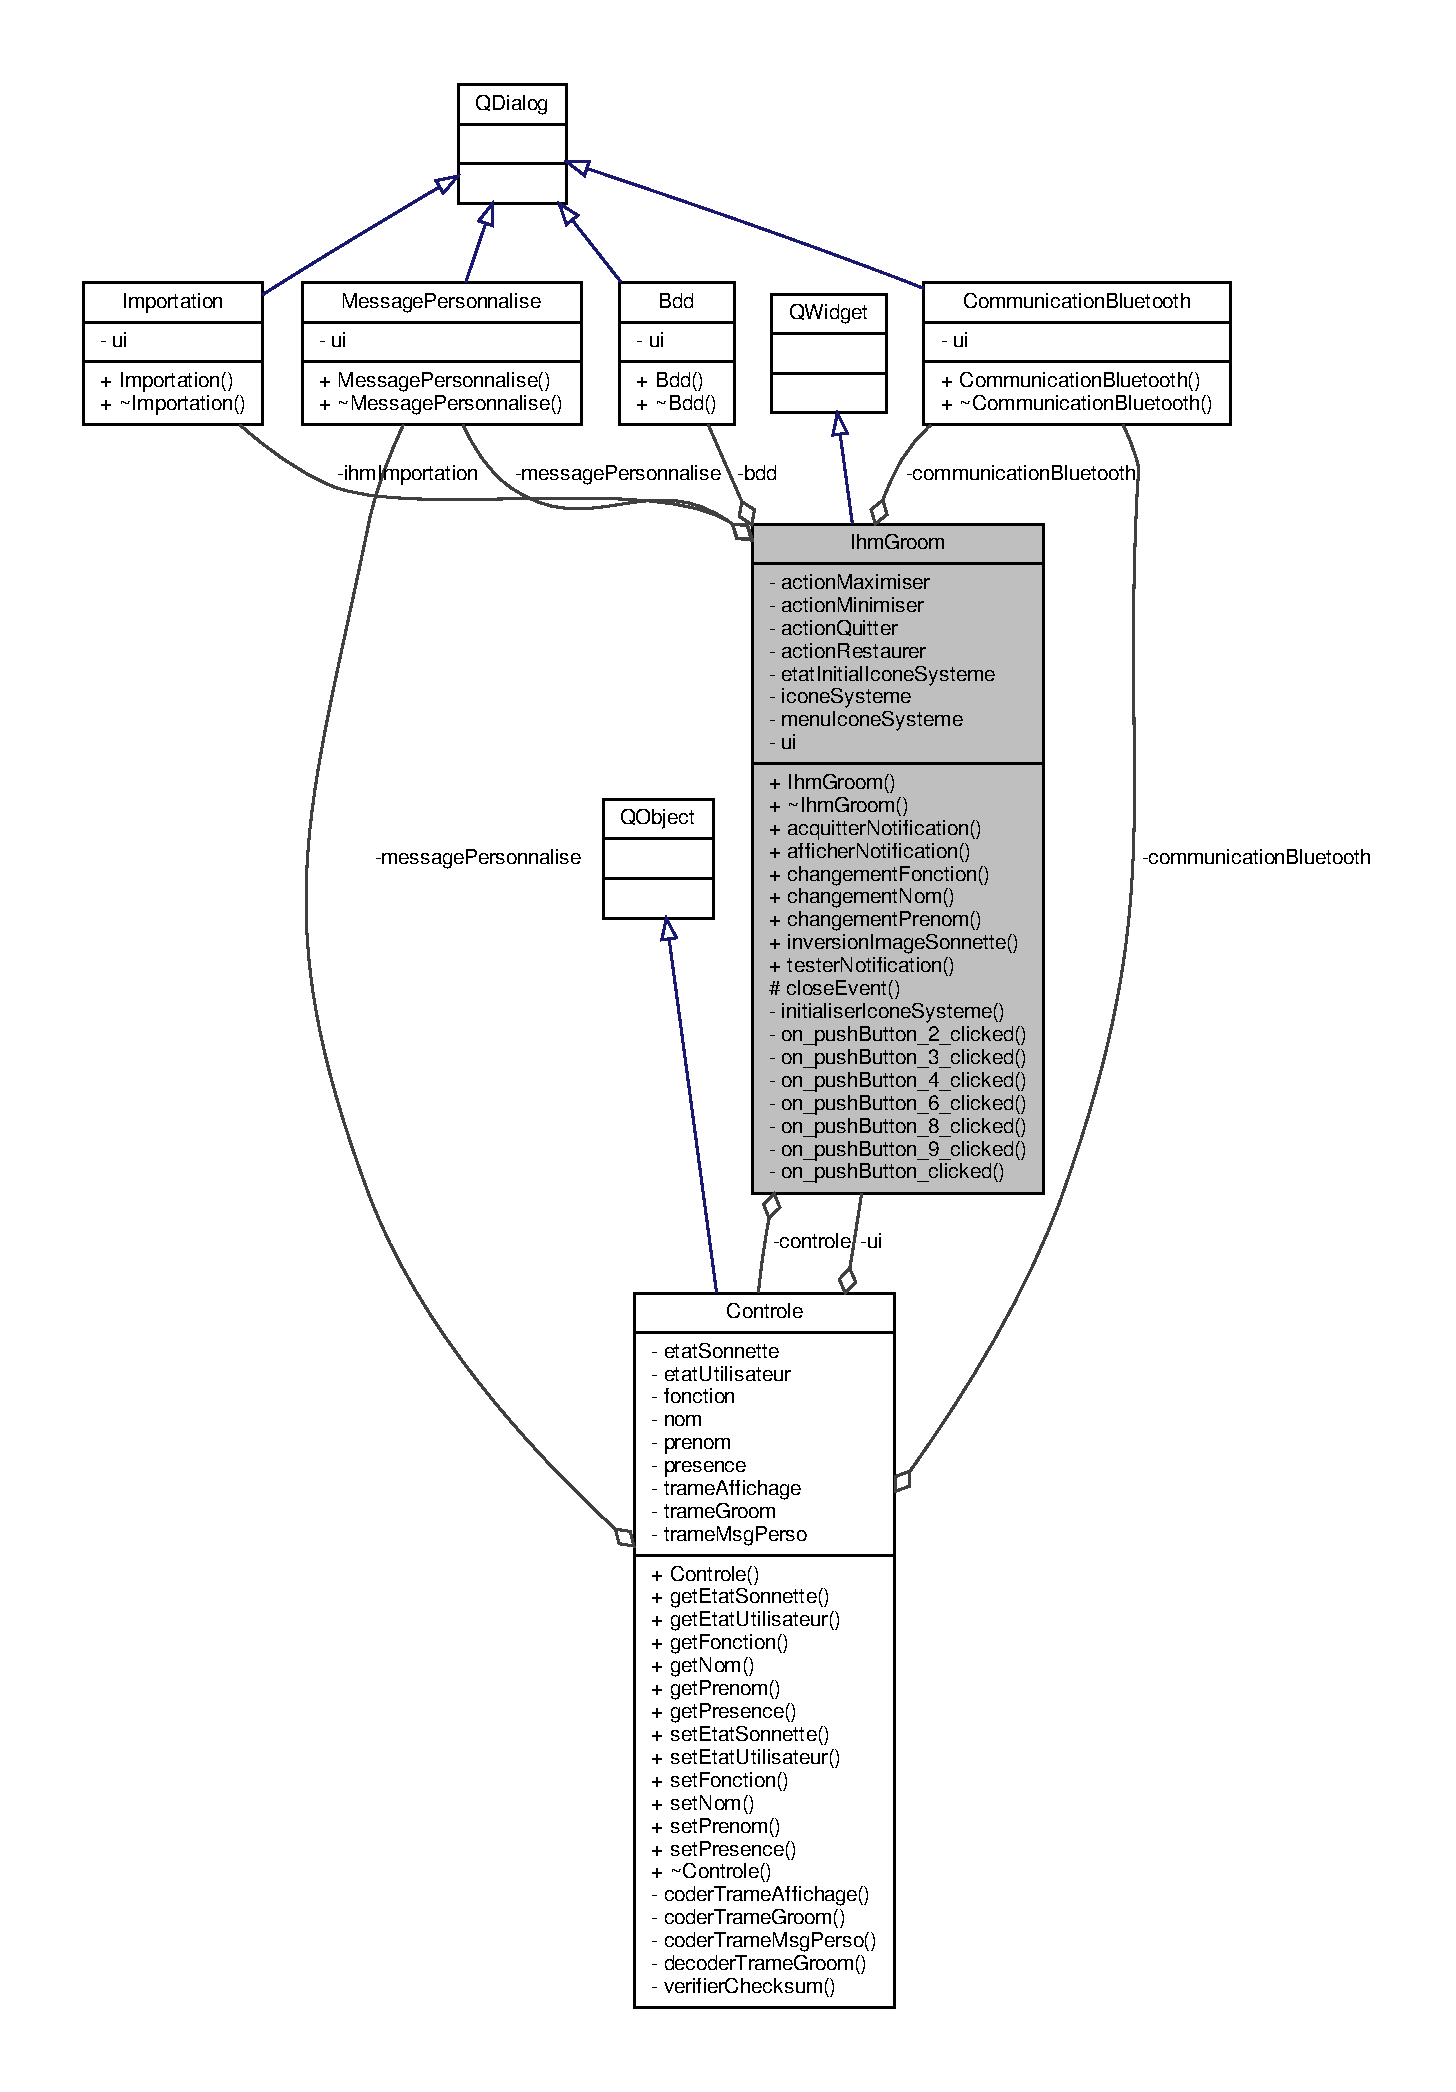
\includegraphics[width=350pt]{class_ihm_groom__coll__graph}
\end{center}
\end{figure}
\subsubsection*{Connecteurs publics}
\begin{DoxyCompactItemize}
\item 
void \hyperlink{class_ihm_groom_a428ffaecbab91abb0824ad61afd3109e}{acquitter\+Notification} ()
\begin{DoxyCompactList}\small\item\em Méthode qui permet d\textquotesingle{}acquitter une notification. \end{DoxyCompactList}\item 
void \hyperlink{class_ihm_groom_a55194db52eca3648aad391274a6bb709}{afficher\+Notification} (Q\+String titre, Q\+String message, int duree=1000)
\begin{DoxyCompactList}\small\item\em Méthode qui permet d\textquotesingle{}afficher une notification système. \end{DoxyCompactList}\item 
void \hyperlink{class_ihm_groom_afc6c48489b270b22a660e32668d6b2ca}{changement\+Fonction} ()
\begin{DoxyCompactList}\small\item\em change la focntion sur l\textquotesingle{}ihm \end{DoxyCompactList}\item 
void \hyperlink{class_ihm_groom_aa270d1fb6a7a9c1385c4ae3e67451ea0}{changement\+Nom} ()
\begin{DoxyCompactList}\small\item\em change le nom sur l\textquotesingle{}ihm \end{DoxyCompactList}\item 
void \hyperlink{class_ihm_groom_a2e8db190224f15326552a5bd642a9347}{changement\+Prenom} ()
\begin{DoxyCompactList}\small\item\em change le prenom sur l\textquotesingle{}ihm \end{DoxyCompactList}\item 
void \hyperlink{class_ihm_groom_a6a7d6102f1d90172215fd4f1aae6e166}{inversion\+Image\+Sonnette} ()
\begin{DoxyCompactList}\small\item\em Inverse l\textquotesingle{}image de la sonnette. \end{DoxyCompactList}\item 
void \hyperlink{class_ihm_groom_a53838a4bd054fe5c85c23eced3eacc8b}{tester\+Notification} ()
\end{DoxyCompactItemize}
\subsubsection*{Fonctions membres publiques}
\begin{DoxyCompactItemize}
\item 
\hyperlink{class_ihm_groom_a44887622008d41828025e2b2ccd598a7}{Ihm\+Groom} (\hyperlink{class_q_widget}{Q\+Widget} $\ast$parent=nullptr)
\begin{DoxyCompactList}\small\item\em Constructeur de la classe \hyperlink{class_ihm_groom}{Ihm\+Groom}. \end{DoxyCompactList}\item 
\hyperlink{class_ihm_groom_a89f5e00d9a36d7162da874b2290274e0}{$\sim$\+Ihm\+Groom} ()
\begin{DoxyCompactList}\small\item\em Destructeur de la classe \hyperlink{class_ihm_groom}{Ihm\+Groom}. \end{DoxyCompactList}\end{DoxyCompactItemize}
\subsubsection*{Fonctions membres protégées}
\begin{DoxyCompactItemize}
\item 
void \hyperlink{class_ihm_groom_a8063930f323ce85b679c7598742f325d}{close\+Event} (Q\+Close\+Event $\ast$event)
\begin{DoxyCompactList}\small\item\em Méthode redéfinie qui est appelée automatiquement lors d\textquotesingle{}une demande de fermeture. \end{DoxyCompactList}\end{DoxyCompactItemize}
\subsubsection*{Connecteurs privés}
\begin{DoxyCompactItemize}
\item 
void \hyperlink{class_ihm_groom_adc890fcb2368c7bf7654d8ed4af4912a}{on\+\_\+push\+Button\+\_\+2\+\_\+clicked} ()
\item 
void \hyperlink{class_ihm_groom_a1d981f0754a5fa2b01036fc5125fded2}{on\+\_\+push\+Button\+\_\+3\+\_\+clicked} ()
\begin{DoxyCompactList}\small\item\em change l\textquotesingle{}état de la personne en Libre \end{DoxyCompactList}\item 
void \hyperlink{class_ihm_groom_addb07bf87d4d6f7eb5604d742a6bf2ef}{on\+\_\+push\+Button\+\_\+4\+\_\+clicked} ()
\item 
void \hyperlink{class_ihm_groom_a1bbde232f2fb38daedaa4562dfc8d1b5}{on\+\_\+push\+Button\+\_\+6\+\_\+clicked} ()
\begin{DoxyCompactList}\small\item\em affiche l\textquotesingle{}ihm communication bluetooth \end{DoxyCompactList}\item 
void \hyperlink{class_ihm_groom_ac69005aef7c31e888d64890eb45c5e64}{on\+\_\+push\+Button\+\_\+8\+\_\+clicked} ()
\begin{DoxyCompactList}\small\item\em affiche l\textquotesingle{}ihm importation \end{DoxyCompactList}\item 
void \hyperlink{class_ihm_groom_a5f8398886e8daa04d5a0f3119f307f14}{on\+\_\+push\+Button\+\_\+9\+\_\+clicked} ()
\item 
void \hyperlink{class_ihm_groom_ad3fbc13397279793b240d54b5a5f20b4}{on\+\_\+push\+Button\+\_\+clicked} ()
\begin{DoxyCompactList}\small\item\em affiche l\textquotesingle{}ihm Message personnalisé \end{DoxyCompactList}\end{DoxyCompactItemize}
\subsubsection*{Fonctions membres privées}
\begin{DoxyCompactItemize}
\item 
void \hyperlink{class_ihm_groom_addfe25c3da6ddecfbdcb5b3cf062d724}{initialiser\+Icone\+Systeme} ()
\begin{DoxyCompactList}\small\item\em Méthode qui permet à l\textquotesingle{}application de s\textquotesingle{}intaller dans la barre système. \end{DoxyCompactList}\end{DoxyCompactItemize}
\subsubsection*{Attributs privés}
\begin{DoxyCompactItemize}
\item 
Q\+Action $\ast$ \hyperlink{class_ihm_groom_aa23dc46d5e223aa20bb84b5bd99d3b81}{action\+Maximiser}
\begin{DoxyCompactList}\small\item\em L\textquotesingle{}action maximiser l\textquotesingle{}application. \end{DoxyCompactList}\item 
Q\+Action $\ast$ \hyperlink{class_ihm_groom_a4018ccf7f73329725e4c54002ae72f01}{action\+Minimiser}
\begin{DoxyCompactList}\small\item\em L\textquotesingle{}action minimiser l\textquotesingle{}application. \end{DoxyCompactList}\item 
Q\+Action $\ast$ \hyperlink{class_ihm_groom_ab28c091688d25e93b2baf99b4aa90f07}{action\+Quitter}
\begin{DoxyCompactList}\small\item\em L\textquotesingle{}action quitter l\textquotesingle{}application. \end{DoxyCompactList}\item 
Q\+Action $\ast$ \hyperlink{class_ihm_groom_aa2df6badfa16f802411b502228fb8704}{action\+Restaurer}
\begin{DoxyCompactList}\small\item\em L\textquotesingle{}action restaurer l\textquotesingle{}application. \end{DoxyCompactList}\item 
\hyperlink{class_bdd}{Bdd} $\ast$ \hyperlink{class_ihm_groom_aba1bfff9bc610e6a626d3af4cec266f9}{bdd}
\item 
\hyperlink{class_communication_bluetooth}{Communication\+Bluetooth} $\ast$ \hyperlink{class_ihm_groom_a8e2b551df75d8dffdfbc9beb6c3691ba}{communication\+Bluetooth}
\begin{DoxyCompactList}\small\item\em L\textquotesingle{}interface de la Configuration. \end{DoxyCompactList}\item 
\hyperlink{class_controle}{Controle} $\ast$ \hyperlink{class_ihm_groom_acead732c303b50a3285bd311ac8a3b4f}{controle}
\item 
bool \hyperlink{class_ihm_groom_a95d2d2b4b3b849c1b21f234844fca056}{etat\+Initial\+Icone\+Systeme}
\begin{DoxyCompactList}\small\item\em Booléen indiquant si c\textquotesingle{}est la première demande Quitter. \end{DoxyCompactList}\item 
Q\+System\+Tray\+Icon $\ast$ \hyperlink{class_ihm_groom_a9ca0929cf284a9a2e3e2bc3489249919}{icone\+Systeme}
\begin{DoxyCompactList}\small\item\em L\textquotesingle{}icône de l\textquotesingle{}application pour la barre système. \end{DoxyCompactList}\item 
\hyperlink{class_importation}{Importation} $\ast$ \hyperlink{class_ihm_groom_ab3f9d16d3e20234a71b1580d70ee4959}{ihm\+Importation}
\begin{DoxyCompactList}\small\item\em L\textquotesingle{}interface de l\textquotesingle{}\hyperlink{class_importation}{Importation}. \end{DoxyCompactList}\item 
Q\+Menu $\ast$ \hyperlink{class_ihm_groom_af2abf22a1a9203af547f32c7edb13710}{menu\+Icone\+Systeme}
\begin{DoxyCompactList}\small\item\em Le menu de l\textquotesingle{}application. \end{DoxyCompactList}\item 
\hyperlink{class_message_personnalise}{Message\+Personnalise} $\ast$ \hyperlink{class_ihm_groom_a529729b93d7b8d17147d3b47fe9a274d}{message\+Personnalise}
\begin{DoxyCompactList}\small\item\em L\textquotesingle{}interface du Message Personnalisé \end{DoxyCompactList}\item 
Ui\+::\+Ihm\+Groom $\ast$ \hyperlink{class_ihm_groom_af652e1ce199213b7867e44cf589c06b8}{ui}
\begin{DoxyCompactList}\small\item\em L\textquotesingle{}interface utilisateur. \end{DoxyCompactList}\end{DoxyCompactItemize}


\subsubsection{Description détaillée}
Déclaration de la classe \hyperlink{class_ihm_groom}{Ihm\+Groom}. 

Définition à la ligne \hyperlink{ihmgroom_8h_source_l00054}{54} du fichier \hyperlink{ihmgroom_8h_source}{ihmgroom.\+h}.



\subsubsection{Documentation des constructeurs et destructeur}
\mbox{\Hypertarget{class_ihm_groom_a44887622008d41828025e2b2ccd598a7}\label{class_ihm_groom_a44887622008d41828025e2b2ccd598a7}} 
\index{Ihm\+Groom@{Ihm\+Groom}!Ihm\+Groom@{Ihm\+Groom}}
\index{Ihm\+Groom@{Ihm\+Groom}!Ihm\+Groom@{Ihm\+Groom}}
\paragraph{\texorpdfstring{Ihm\+Groom()}{IhmGroom()}}
{\footnotesize\ttfamily Ihm\+Groom\+::\+Ihm\+Groom (\begin{DoxyParamCaption}\item[{\hyperlink{class_q_widget}{Q\+Widget} $\ast$}]{parent = {\ttfamily nullptr} }\end{DoxyParamCaption})\hspace{0.3cm}{\ttfamily [explicit]}}



Constructeur de la classe \hyperlink{class_ihm_groom}{Ihm\+Groom}. 

Constructeur classe \hyperlink{class_ihm_groom}{Ihm\+Groom}.


\begin{DoxyParams}{Paramètres}
{\em parent} & L\textquotesingle{}objet parent Qt (0 = fenêtre principale)\\
\hline
{\em parent} & \\
\hline
\end{DoxyParams}
\begin{DoxyRefDesc}{A faire}
\item[\hyperlink{todo__todo000001}{A faire}]Renommer les widgets \end{DoxyRefDesc}


Définition à la ligne \hyperlink{ihmgroom_8cpp_source_l00031}{31} du fichier \hyperlink{ihmgroom_8cpp_source}{ihmgroom.\+cpp}.



Références \hyperlink{ihmgroom_8h_source_l00090}{bdd}, \hyperlink{ihmgroom_8h_source_l00086}{communication\+Bluetooth}, \hyperlink{ihmgroom_8h_source_l00089}{controle}, \hyperlink{ihmgroom_8h_source_l00087}{ihm\+Importation}, \hyperlink{ihmgroom_8cpp_source_l00106}{initialiser\+Icone\+Systeme()}, \hyperlink{ihmgroom_8cpp_source_l00201}{inversion\+Image\+Sonnette()}, \hyperlink{ihmgroom_8h_source_l00088}{message\+Personnalise}, \hyperlink{ihmgroom_8h_source_l00018}{N\+O\+M\+\_\+\+A\+PP}, \hyperlink{ihmgroom_8cpp_source_l00175}{tester\+Notification()}, et \hyperlink{ihmgroom_8h_source_l00085}{ui}.


\begin{DoxyCode}
00031                                   : \hyperlink{class_q_widget}{QWidget}(parent), \hyperlink{class_ihm_groom_af652e1ce199213b7867e44cf589c06b8}{ui}(\textcolor{keyword}{new} Ui::IhmGroom)
00032 \{
00033     qDebug() << Q\_FUNC\_INFO;
00034     \hyperlink{class_ihm_groom_af652e1ce199213b7867e44cf589c06b8}{ui}->setupUi(\textcolor{keyword}{this});
00035     setWindowTitle(\hyperlink{ihmgroom_8h_ada54de88f03c1264af632974a72cff76}{NOM\_APP});
00036 
00037     \hyperlink{class_ihm_groom_ab3f9d16d3e20234a71b1580d70ee4959}{ihmImportation} = \textcolor{keyword}{new} \hyperlink{class_importation}{Importation}(\textcolor{keyword}{this});
00038     \hyperlink{class_ihm_groom_a529729b93d7b8d17147d3b47fe9a274d}{messagePersonnalise} = \textcolor{keyword}{new} \hyperlink{class_message_personnalise}{MessagePersonnalise}(\textcolor{keyword}{this});
00039     \hyperlink{class_ihm_groom_a8e2b551df75d8dffdfbc9beb6c3691ba}{communicationBluetooth} = \textcolor{keyword}{new} \hyperlink{class_communication_bluetooth}{CommunicationBluetooth}(\textcolor{keyword}{this});
00040     \hyperlink{class_ihm_groom_acead732c303b50a3285bd311ac8a3b4f}{controle} = \textcolor{keyword}{new} \hyperlink{class_controle}{Controle}(\textcolor{keyword}{this});
00041     \hyperlink{class_ihm_groom_aba1bfff9bc610e6a626d3af4cec266f9}{bdd} = \textcolor{keyword}{new} \hyperlink{class_bdd}{Bdd}(\textcolor{keyword}{this});
00042 
00043     \hyperlink{class_ihm_groom_addfe25c3da6ddecfbdcb5b3cf062d724}{initialiserIconeSysteme}();
00044     connect(\hyperlink{class_ihm_groom_af652e1ce199213b7867e44cf589c06b8}{ui}->pushButton\_5, SIGNAL(clicked()), \textcolor{keyword}{this}, SLOT(
      \hyperlink{class_ihm_groom_a6a7d6102f1d90172215fd4f1aae6e166}{inversionImageSonnette}()));
00048     \textcolor{comment}{// Test :}
00049     connect(\hyperlink{class_ihm_groom_af652e1ce199213b7867e44cf589c06b8}{ui}->pushButton\_7, SIGNAL(clicked()), \textcolor{keyword}{this}, SLOT(\hyperlink{class_ihm_groom_a53838a4bd054fe5c85c23eced3eacc8b}{testerNotification}()));
00050     connect(\hyperlink{class_ihm_groom_af652e1ce199213b7867e44cf589c06b8}{ui}->pushButton\_6, SIGNAL(clicked()), \textcolor{keyword}{this}, SLOT(afficherIhmConfiguration()));
00051 
00052 \}
\end{DoxyCode}
\mbox{\Hypertarget{class_ihm_groom_a89f5e00d9a36d7162da874b2290274e0}\label{class_ihm_groom_a89f5e00d9a36d7162da874b2290274e0}} 
\index{Ihm\+Groom@{Ihm\+Groom}!````~Ihm\+Groom@{$\sim$\+Ihm\+Groom}}
\index{````~Ihm\+Groom@{$\sim$\+Ihm\+Groom}!Ihm\+Groom@{Ihm\+Groom}}
\paragraph{\texorpdfstring{$\sim$\+Ihm\+Groom()}{~IhmGroom()}}
{\footnotesize\ttfamily Ihm\+Groom\+::$\sim$\+Ihm\+Groom (\begin{DoxyParamCaption}{ }\end{DoxyParamCaption})}



Destructeur de la classe \hyperlink{class_ihm_groom}{Ihm\+Groom}. 

Constructeur classe $\sim$\+Ihm\+Groom.


\begin{DoxyParams}{Paramètres}
{\em parent} & \\
\hline
\end{DoxyParams}


Définition à la ligne \hyperlink{ihmgroom_8cpp_source_l00059}{59} du fichier \hyperlink{ihmgroom_8cpp_source}{ihmgroom.\+cpp}.



Références \hyperlink{ihmgroom_8h_source_l00085}{ui}.


\begin{DoxyCode}
00060 \{
00061     \textcolor{keyword}{delete} \hyperlink{class_ihm_groom_af652e1ce199213b7867e44cf589c06b8}{ui};
00062      qDebug() << Q\_FUNC\_INFO;
00063 \}
\end{DoxyCode}


\subsubsection{Documentation des fonctions membres}
\mbox{\Hypertarget{class_ihm_groom_a428ffaecbab91abb0824ad61afd3109e}\label{class_ihm_groom_a428ffaecbab91abb0824ad61afd3109e}} 
\index{Ihm\+Groom@{Ihm\+Groom}!acquitter\+Notification@{acquitter\+Notification}}
\index{acquitter\+Notification@{acquitter\+Notification}!Ihm\+Groom@{Ihm\+Groom}}
\paragraph{\texorpdfstring{acquitter\+Notification}{acquitterNotification}}
{\footnotesize\ttfamily Ihm\+Groom\+::acquitter\+Notification (\begin{DoxyParamCaption}{ }\end{DoxyParamCaption})\hspace{0.3cm}{\ttfamily [slot]}}



Méthode qui permet d\textquotesingle{}acquitter une notification. 

Acquitter les notification. 

Définition à la ligne \hyperlink{ihmgroom_8cpp_source_l00170}{170} du fichier \hyperlink{ihmgroom_8cpp_source}{ihmgroom.\+cpp}.



Référencé par \hyperlink{ihmgroom_8cpp_source_l00106}{initialiser\+Icone\+Systeme()}.


\begin{DoxyCode}
00171 \{
00172     qDebug() << Q\_FUNC\_INFO;
00173 \}
\end{DoxyCode}
\mbox{\Hypertarget{class_ihm_groom_a55194db52eca3648aad391274a6bb709}\label{class_ihm_groom_a55194db52eca3648aad391274a6bb709}} 
\index{Ihm\+Groom@{Ihm\+Groom}!afficher\+Notification@{afficher\+Notification}}
\index{afficher\+Notification@{afficher\+Notification}!Ihm\+Groom@{Ihm\+Groom}}
\paragraph{\texorpdfstring{afficher\+Notification}{afficherNotification}}
{\footnotesize\ttfamily Ihm\+Groom\+::afficher\+Notification (\begin{DoxyParamCaption}\item[{Q\+String}]{titre,  }\item[{Q\+String}]{message,  }\item[{int}]{duree = {\ttfamily 1000} }\end{DoxyParamCaption})\hspace{0.3cm}{\ttfamily [slot]}}



Méthode qui permet d\textquotesingle{}afficher une notification système. 

Affichage des notification.


\begin{DoxyParams}{Paramètres}
{\em titre} & Le titre de la notification \\
\hline
{\em message} & Le message de la notification \\
\hline
{\em duree} & La durée en millisecondes de la notification (par défaut 5s) \\
\hline
\end{DoxyParams}


Définition à la ligne \hyperlink{ihmgroom_8cpp_source_l00151}{151} du fichier \hyperlink{ihmgroom_8cpp_source}{ihmgroom.\+cpp}.



Références \hyperlink{ihmgroom_8h_source_l00093}{icone\+Systeme}.



Référencé par \hyperlink{ihmgroom_8cpp_source_l00175}{tester\+Notification()}.


\begin{DoxyCode}
00152 \{
00153     QIcon icone(\textcolor{stringliteral}{":/groom.png"});
00154     \hyperlink{class_ihm_groom_a9ca0929cf284a9a2e3e2bc3489249919}{iconeSysteme}->showMessage(titre, message, icone, duree); \textcolor{comment}{// duree en ms}
00155     \textcolor{comment}{/*}
00156 \textcolor{comment}{    QSystemTrayIcon::NoIcon}
00157 \textcolor{comment}{    QSystemTrayIcon::Information}
00158 \textcolor{comment}{    QSystemTrayIcon::Warning}
00159 \textcolor{comment}{    QSystemTrayIcon::Critical}
00160 \textcolor{comment}{    */}
00161     \textcolor{comment}{//QSystemTrayIcon::MessageIcon messageIcone =
       QSystemTrayIcon::MessageIcon(QSystemTrayIcon::Information);}
00162     \textcolor{comment}{//iconeSysteme->showMessage(titre, message, messageIcone, duree);}
00163 \}
\end{DoxyCode}
\mbox{\Hypertarget{class_ihm_groom_afc6c48489b270b22a660e32668d6b2ca}\label{class_ihm_groom_afc6c48489b270b22a660e32668d6b2ca}} 
\index{Ihm\+Groom@{Ihm\+Groom}!changement\+Fonction@{changement\+Fonction}}
\index{changement\+Fonction@{changement\+Fonction}!Ihm\+Groom@{Ihm\+Groom}}
\paragraph{\texorpdfstring{changement\+Fonction}{changementFonction}}
{\footnotesize\ttfamily Ihm\+Groom\+::changement\+Fonction (\begin{DoxyParamCaption}{ }\end{DoxyParamCaption})\hspace{0.3cm}{\ttfamily [slot]}}



change la focntion sur l\textquotesingle{}ihm 



Définition à la ligne \hyperlink{ihmgroom_8cpp_source_l00075}{75} du fichier \hyperlink{ihmgroom_8cpp_source}{ihmgroom.\+cpp}.



Références \hyperlink{ihmgroom_8h_source_l00089}{controle}, \hyperlink{controle_8cpp_source_l00096}{Controle\+::get\+Fonction()}, et \hyperlink{ihmgroom_8h_source_l00085}{ui}.



Référencé par \hyperlink{controle_8cpp_source_l00101}{Controle\+::coder\+Trame\+Affichage()}.


\begin{DoxyCode}
00076 \{
00077     \hyperlink{class_ihm_groom_af652e1ce199213b7867e44cf589c06b8}{ui}->label\_Fonction->setWindowTitle(\hyperlink{class_ihm_groom_acead732c303b50a3285bd311ac8a3b4f}{controle}->\hyperlink{class_controle_a8d2891b2b01c503d10f775b4b14a3777}{getFonction}());
00078 \}
\end{DoxyCode}
\mbox{\Hypertarget{class_ihm_groom_aa270d1fb6a7a9c1385c4ae3e67451ea0}\label{class_ihm_groom_aa270d1fb6a7a9c1385c4ae3e67451ea0}} 
\index{Ihm\+Groom@{Ihm\+Groom}!changement\+Nom@{changement\+Nom}}
\index{changement\+Nom@{changement\+Nom}!Ihm\+Groom@{Ihm\+Groom}}
\paragraph{\texorpdfstring{changement\+Nom}{changementNom}}
{\footnotesize\ttfamily Ihm\+Groom\+::changement\+Nom (\begin{DoxyParamCaption}{ }\end{DoxyParamCaption})\hspace{0.3cm}{\ttfamily [slot]}}



change le nom sur l\textquotesingle{}ihm 



Définition à la ligne \hyperlink{ihmgroom_8cpp_source_l00065}{65} du fichier \hyperlink{ihmgroom_8cpp_source}{ihmgroom.\+cpp}.



Références \hyperlink{ihmgroom_8h_source_l00089}{controle}, \hyperlink{controle_8cpp_source_l00080}{Controle\+::get\+Nom()}, et \hyperlink{ihmgroom_8h_source_l00085}{ui}.



Référencé par \hyperlink{controle_8cpp_source_l00101}{Controle\+::coder\+Trame\+Affichage()}.


\begin{DoxyCode}
00066 \{
00067     \hyperlink{class_ihm_groom_af652e1ce199213b7867e44cf589c06b8}{ui}->label\_Nom->setWindowTitle(\hyperlink{class_ihm_groom_acead732c303b50a3285bd311ac8a3b4f}{controle}->\hyperlink{class_controle_ac6e8590a5108e97fce3ce3aa43feb881}{getNom}());
00068 \}
\end{DoxyCode}
\mbox{\Hypertarget{class_ihm_groom_a2e8db190224f15326552a5bd642a9347}\label{class_ihm_groom_a2e8db190224f15326552a5bd642a9347}} 
\index{Ihm\+Groom@{Ihm\+Groom}!changement\+Prenom@{changement\+Prenom}}
\index{changement\+Prenom@{changement\+Prenom}!Ihm\+Groom@{Ihm\+Groom}}
\paragraph{\texorpdfstring{changement\+Prenom}{changementPrenom}}
{\footnotesize\ttfamily Ihm\+Groom\+::changement\+Prenom (\begin{DoxyParamCaption}{ }\end{DoxyParamCaption})\hspace{0.3cm}{\ttfamily [slot]}}



change le prenom sur l\textquotesingle{}ihm 



Définition à la ligne \hyperlink{ihmgroom_8cpp_source_l00070}{70} du fichier \hyperlink{ihmgroom_8cpp_source}{ihmgroom.\+cpp}.



Références \hyperlink{ihmgroom_8h_source_l00089}{controle}, \hyperlink{controle_8cpp_source_l00088}{Controle\+::get\+Prenom()}, et \hyperlink{ihmgroom_8h_source_l00085}{ui}.



Référencé par \hyperlink{controle_8cpp_source_l00101}{Controle\+::coder\+Trame\+Affichage()}.


\begin{DoxyCode}
00071 \{
00072     \hyperlink{class_ihm_groom_af652e1ce199213b7867e44cf589c06b8}{ui}->label\_Prenom->setWindowTitle(\hyperlink{class_ihm_groom_acead732c303b50a3285bd311ac8a3b4f}{controle}->\hyperlink{class_controle_a0164fd9066b1703498576095ab5642c5}{getPrenom}());
00073 \}
\end{DoxyCode}
\mbox{\Hypertarget{class_ihm_groom_a8063930f323ce85b679c7598742f325d}\label{class_ihm_groom_a8063930f323ce85b679c7598742f325d}} 
\index{Ihm\+Groom@{Ihm\+Groom}!close\+Event@{close\+Event}}
\index{close\+Event@{close\+Event}!Ihm\+Groom@{Ihm\+Groom}}
\paragraph{\texorpdfstring{close\+Event()}{closeEvent()}}
{\footnotesize\ttfamily void Ihm\+Groom\+::close\+Event (\begin{DoxyParamCaption}\item[{Q\+Close\+Event $\ast$}]{event }\end{DoxyParamCaption})\hspace{0.3cm}{\ttfamily [protected]}}



Méthode redéfinie qui est appelée automatiquement lors d\textquotesingle{}une demande de fermeture. 


\begin{DoxyParams}{Paramètres}
{\em event} & L\textquotesingle{}évènement de fermeture reçu \\
\hline
\end{DoxyParams}


Définition à la ligne \hyperlink{ihmgroom_8cpp_source_l00087}{87} du fichier \hyperlink{ihmgroom_8cpp_source}{ihmgroom.\+cpp}.



Références \hyperlink{ihmgroom_8h_source_l00099}{etat\+Initial\+Icone\+Systeme}, et \hyperlink{ihmgroom_8h_source_l00093}{icone\+Systeme}.


\begin{DoxyCode}
00088 \{
00089     \textcolor{keywordflow}{if} (\hyperlink{class_ihm_groom_a9ca0929cf284a9a2e3e2bc3489249919}{iconeSysteme}->isVisible())
00090     \{
00091         \textcolor{keywordflow}{if}(\hyperlink{class_ihm_groom_a95d2d2b4b3b849c1b21f234844fca056}{etatInitialIconeSysteme})
00092         \{
00093             QMessageBox::information(\textcolor{keyword}{this}, \textcolor{stringliteral}{"Groom"}, \textcolor{stringliteral}{"Le programme continue à s'éxécuter. Utiliser le menu
       Quitter pour mettre fin à l'application Groom."});
00094             \hyperlink{class_ihm_groom_a95d2d2b4b3b849c1b21f234844fca056}{etatInitialIconeSysteme} = \textcolor{keyword}{false};
00095         \}
00096         hide();
00097         \textcolor{keyword}{event}->ignore();
00098     \}
00099 \}
\end{DoxyCode}
\mbox{\Hypertarget{class_ihm_groom_addfe25c3da6ddecfbdcb5b3cf062d724}\label{class_ihm_groom_addfe25c3da6ddecfbdcb5b3cf062d724}} 
\index{Ihm\+Groom@{Ihm\+Groom}!initialiser\+Icone\+Systeme@{initialiser\+Icone\+Systeme}}
\index{initialiser\+Icone\+Systeme@{initialiser\+Icone\+Systeme}!Ihm\+Groom@{Ihm\+Groom}}
\paragraph{\texorpdfstring{initialiser\+Icone\+Systeme()}{initialiserIconeSysteme()}}
{\footnotesize\ttfamily Ihm\+Groom\+::initialiser\+Icone\+Systeme (\begin{DoxyParamCaption}{ }\end{DoxyParamCaption})\hspace{0.3cm}{\ttfamily [private]}}



Méthode qui permet à l\textquotesingle{}application de s\textquotesingle{}intaller dans la barre système. 

Affichage dans barre des taches. 

Définition à la ligne \hyperlink{ihmgroom_8cpp_source_l00106}{106} du fichier \hyperlink{ihmgroom_8cpp_source}{ihmgroom.\+cpp}.



Références \hyperlink{ihmgroom_8cpp_source_l00170}{acquitter\+Notification()}, \hyperlink{ihmgroom_8h_source_l00096}{action\+Maximiser}, \hyperlink{ihmgroom_8h_source_l00095}{action\+Minimiser}, \hyperlink{ihmgroom_8h_source_l00098}{action\+Quitter}, \hyperlink{ihmgroom_8h_source_l00097}{action\+Restaurer}, \hyperlink{ihmgroom_8h_source_l00099}{etat\+Initial\+Icone\+Systeme}, \hyperlink{ihmgroom_8h_source_l00093}{icone\+Systeme}, et \hyperlink{ihmgroom_8h_source_l00094}{menu\+Icone\+Systeme}.



Référencé par \hyperlink{ihmgroom_8cpp_source_l00031}{Ihm\+Groom()}.


\begin{DoxyCode}
00107 \{
00108     \textcolor{comment}{// Crée les actions}
00109     \hyperlink{class_ihm_groom_a4018ccf7f73329725e4c54002ae72f01}{actionMinimiser} = \textcolor{keyword}{new} QAction(QString::fromUtf8(\textcolor{stringliteral}{"Minimiser"}), \textcolor{keyword}{this});
00110     \hyperlink{class_ihm_groom_aa23dc46d5e223aa20bb84b5bd99d3b81}{actionMaximiser} = \textcolor{keyword}{new} QAction(QString::fromUtf8(\textcolor{stringliteral}{"Maximiser"}), \textcolor{keyword}{this});
00111     \hyperlink{class_ihm_groom_aa2df6badfa16f802411b502228fb8704}{actionRestaurer} = \textcolor{keyword}{new} QAction(QString::fromUtf8(\textcolor{stringliteral}{"Restaurer"}), \textcolor{keyword}{this});
00112     \hyperlink{class_ihm_groom_ab28c091688d25e93b2baf99b4aa90f07}{actionQuitter} = \textcolor{keyword}{new} QAction(QString::fromUtf8(\textcolor{stringliteral}{"&Quitter"}), \textcolor{keyword}{this});
00113 
00114     \textcolor{comment}{// Connecte les actions}
00115     connect(\hyperlink{class_ihm_groom_a4018ccf7f73329725e4c54002ae72f01}{actionMinimiser}, SIGNAL(triggered(\textcolor{keywordtype}{bool})), \textcolor{keyword}{this}, SLOT(hide()));
00116     connect(\hyperlink{class_ihm_groom_aa23dc46d5e223aa20bb84b5bd99d3b81}{actionMaximiser}, SIGNAL(triggered(\textcolor{keywordtype}{bool})), \textcolor{keyword}{this}, SLOT(showMaximized()));
00117     connect(\hyperlink{class_ihm_groom_aa2df6badfa16f802411b502228fb8704}{actionRestaurer}, SIGNAL(triggered(\textcolor{keywordtype}{bool})), \textcolor{keyword}{this}, SLOT(showNormal()));
00118     connect(\hyperlink{class_ihm_groom_ab28c091688d25e93b2baf99b4aa90f07}{actionQuitter}, SIGNAL(triggered(\textcolor{keywordtype}{bool})), qApp, SLOT(quit()));
00119 
00120     \textcolor{comment}{// Crée le menu}
00121     \hyperlink{class_ihm_groom_af2abf22a1a9203af547f32c7edb13710}{menuIconeSysteme} = \textcolor{keyword}{new} QMenu(\textcolor{keyword}{this});
00122     \hyperlink{class_ihm_groom_af2abf22a1a9203af547f32c7edb13710}{menuIconeSysteme}->addAction(\hyperlink{class_ihm_groom_a4018ccf7f73329725e4c54002ae72f01}{actionMinimiser});
00123     \hyperlink{class_ihm_groom_af2abf22a1a9203af547f32c7edb13710}{menuIconeSysteme}->addAction(\hyperlink{class_ihm_groom_aa23dc46d5e223aa20bb84b5bd99d3b81}{actionMaximiser});
00124     \hyperlink{class_ihm_groom_af2abf22a1a9203af547f32c7edb13710}{menuIconeSysteme}->addAction(\hyperlink{class_ihm_groom_aa2df6badfa16f802411b502228fb8704}{actionRestaurer});
00125     \hyperlink{class_ihm_groom_af2abf22a1a9203af547f32c7edb13710}{menuIconeSysteme}->addSeparator();
00126     \hyperlink{class_ihm_groom_af2abf22a1a9203af547f32c7edb13710}{menuIconeSysteme}->addAction(\hyperlink{class_ihm_groom_ab28c091688d25e93b2baf99b4aa90f07}{actionQuitter});
00127 
00128     \textcolor{comment}{// Crée l'icône pour la barre de tâche}
00129     \hyperlink{class_ihm_groom_a9ca0929cf284a9a2e3e2bc3489249919}{iconeSysteme} = \textcolor{keyword}{new} QSystemTrayIcon(\textcolor{keyword}{this});
00130     \hyperlink{class_ihm_groom_a9ca0929cf284a9a2e3e2bc3489249919}{iconeSysteme}->setContextMenu(\hyperlink{class_ihm_groom_af2abf22a1a9203af547f32c7edb13710}{menuIconeSysteme});
00131     \hyperlink{class_ihm_groom_a9ca0929cf284a9a2e3e2bc3489249919}{iconeSysteme}->setToolTip(\textcolor{stringliteral}{"Groom"});
00132     QIcon icone(\textcolor{stringliteral}{":/groom.png"});
00133     \hyperlink{class_ihm_groom_a9ca0929cf284a9a2e3e2bc3489249919}{iconeSysteme}->setIcon(icone);
00134     setWindowIcon(icone);
00135 
00136     connect(\hyperlink{class_ihm_groom_a9ca0929cf284a9a2e3e2bc3489249919}{iconeSysteme}, SIGNAL(messageClicked()), \textcolor{keyword}{this}, SLOT(
      \hyperlink{class_ihm_groom_a428ffaecbab91abb0824ad61afd3109e}{acquitterNotification}()));
00137     \textcolor{comment}{//connect(iconeSysteme, SIGNAL(activated(QSystemTrayIcon::ActivationReason)), this,
       SLOT(aActiveIconeSysteme(QSystemTrayIcon::ActivationReason)));}
00138 
00139     \hyperlink{class_ihm_groom_a9ca0929cf284a9a2e3e2bc3489249919}{iconeSysteme}->show();
00140     \hyperlink{class_ihm_groom_a95d2d2b4b3b849c1b21f234844fca056}{etatInitialIconeSysteme} = \textcolor{keyword}{true};
00141 \}
\end{DoxyCode}
\mbox{\Hypertarget{class_ihm_groom_a6a7d6102f1d90172215fd4f1aae6e166}\label{class_ihm_groom_a6a7d6102f1d90172215fd4f1aae6e166}} 
\index{Ihm\+Groom@{Ihm\+Groom}!inversion\+Image\+Sonnette@{inversion\+Image\+Sonnette}}
\index{inversion\+Image\+Sonnette@{inversion\+Image\+Sonnette}!Ihm\+Groom@{Ihm\+Groom}}
\paragraph{\texorpdfstring{inversion\+Image\+Sonnette}{inversionImageSonnette}}
{\footnotesize\ttfamily Ihm\+Groom\+::inversion\+Image\+Sonnette (\begin{DoxyParamCaption}{ }\end{DoxyParamCaption})\hspace{0.3cm}{\ttfamily [slot]}}



Inverse l\textquotesingle{}image de la sonnette. 



Définition à la ligne \hyperlink{ihmgroom_8cpp_source_l00201}{201} du fichier \hyperlink{ihmgroom_8cpp_source}{ihmgroom.\+cpp}.



Références \hyperlink{ihmgroom_8h_source_l00089}{controle}, \hyperlink{controle_8cpp_source_l00033}{Controle\+::get\+Etat\+Sonnette()}, \hyperlink{controle_8cpp_source_l00028}{Controle\+::set\+Etat\+Sonnette()}, et \hyperlink{ihmgroom_8h_source_l00085}{ui}.



Référencé par \hyperlink{ihmgroom_8cpp_source_l00031}{Ihm\+Groom()}.


\begin{DoxyCode}
00202 \{
00203 
00204     \textcolor{keywordflow}{if} (\hyperlink{class_ihm_groom_acead732c303b50a3285bd311ac8a3b4f}{controle}->\hyperlink{class_controle_acabf3768430c7f1acb268ca0fa1ddf99}{getEtatSonnette}())
00205     \{
00206         \hyperlink{class_ihm_groom_af652e1ce199213b7867e44cf589c06b8}{ui}->pushButton\_5->setIcon(QIcon(\textcolor{stringliteral}{":/bellDisable.png"}));
00207 
00208         \hyperlink{class_ihm_groom_acead732c303b50a3285bd311ac8a3b4f}{controle}->\hyperlink{class_controle_ac706c5e9ede46dab70631281b084e233}{setEtatSonnette}(\textcolor{keyword}{false});
00209 
00210     \}
00211     \textcolor{keywordflow}{else}
00212     \{
00213         \hyperlink{class_ihm_groom_af652e1ce199213b7867e44cf589c06b8}{ui}->pushButton\_5->setIcon(QIcon(\textcolor{stringliteral}{":/bellEnable.png"}));
00214         \hyperlink{class_ihm_groom_acead732c303b50a3285bd311ac8a3b4f}{controle}->\hyperlink{class_controle_ac706c5e9ede46dab70631281b084e233}{setEtatSonnette}(\textcolor{keyword}{true});
00215     \}
00216 \}
\end{DoxyCode}
\mbox{\Hypertarget{class_ihm_groom_adc890fcb2368c7bf7654d8ed4af4912a}\label{class_ihm_groom_adc890fcb2368c7bf7654d8ed4af4912a}} 
\index{Ihm\+Groom@{Ihm\+Groom}!on\+\_\+push\+Button\+\_\+2\+\_\+clicked@{on\+\_\+push\+Button\+\_\+2\+\_\+clicked}}
\index{on\+\_\+push\+Button\+\_\+2\+\_\+clicked@{on\+\_\+push\+Button\+\_\+2\+\_\+clicked}!Ihm\+Groom@{Ihm\+Groom}}
\paragraph{\texorpdfstring{on\+\_\+push\+Button\+\_\+2\+\_\+clicked}{on\_pushButton\_2\_clicked}}
{\footnotesize\ttfamily void Ihm\+Groom\+::on\+\_\+push\+Button\+\_\+2\+\_\+clicked (\begin{DoxyParamCaption}{ }\end{DoxyParamCaption})\hspace{0.3cm}{\ttfamily [private]}, {\ttfamily [slot]}}



Définition à la ligne \hyperlink{ihmgroom_8cpp_source_l00229}{229} du fichier \hyperlink{ihmgroom_8cpp_source}{ihmgroom.\+cpp}.



Références \hyperlink{ihmgroom_8h_source_l00030}{A\+B\+S\+E\+NT}, \hyperlink{ihmgroom_8h_source_l00089}{controle}, et \hyperlink{controle_8cpp_source_l00018}{Controle\+::set\+Etat\+Utilisateur()}.


\begin{DoxyCode}
00230 \{
00231     \hyperlink{class_ihm_groom_acead732c303b50a3285bd311ac8a3b4f}{controle}->\hyperlink{class_controle_a62db54114d126d03dd332332b3942320}{setEtatUtilisateur}(\hyperlink{ihmgroom_8h_a62d1ab4a9b5e2f95388be50a975cc97d}{ABSENT});
00232 \}
\end{DoxyCode}
\mbox{\Hypertarget{class_ihm_groom_a1d981f0754a5fa2b01036fc5125fded2}\label{class_ihm_groom_a1d981f0754a5fa2b01036fc5125fded2}} 
\index{Ihm\+Groom@{Ihm\+Groom}!on\+\_\+push\+Button\+\_\+3\+\_\+clicked@{on\+\_\+push\+Button\+\_\+3\+\_\+clicked}}
\index{on\+\_\+push\+Button\+\_\+3\+\_\+clicked@{on\+\_\+push\+Button\+\_\+3\+\_\+clicked}!Ihm\+Groom@{Ihm\+Groom}}
\paragraph{\texorpdfstring{on\+\_\+push\+Button\+\_\+3\+\_\+clicked}{on\_pushButton\_3\_clicked}}
{\footnotesize\ttfamily Ihm\+Groom\+::on\+\_\+push\+Button\+\_\+3\+\_\+clicked (\begin{DoxyParamCaption}{ }\end{DoxyParamCaption})\hspace{0.3cm}{\ttfamily [private]}, {\ttfamily [slot]}}



change l\textquotesingle{}état de la personne en Libre 



Définition à la ligne \hyperlink{ihmgroom_8cpp_source_l00219}{219} du fichier \hyperlink{ihmgroom_8cpp_source}{ihmgroom.\+cpp}.



Références \hyperlink{ihmgroom_8h_source_l00089}{controle}, \hyperlink{ihmgroom_8h_source_l00024}{L\+I\+B\+RE}, et \hyperlink{controle_8cpp_source_l00018}{Controle\+::set\+Etat\+Utilisateur()}.


\begin{DoxyCode}
00220 \{
00221     \hyperlink{class_ihm_groom_acead732c303b50a3285bd311ac8a3b4f}{controle}->\hyperlink{class_controle_a62db54114d126d03dd332332b3942320}{setEtatUtilisateur}(\hyperlink{ihmgroom_8h_a508cc209fbc99ea975d1c1ecb5f1c6fe}{LIBRE});
00222 \}
\end{DoxyCode}
\mbox{\Hypertarget{class_ihm_groom_addb07bf87d4d6f7eb5604d742a6bf2ef}\label{class_ihm_groom_addb07bf87d4d6f7eb5604d742a6bf2ef}} 
\index{Ihm\+Groom@{Ihm\+Groom}!on\+\_\+push\+Button\+\_\+4\+\_\+clicked@{on\+\_\+push\+Button\+\_\+4\+\_\+clicked}}
\index{on\+\_\+push\+Button\+\_\+4\+\_\+clicked@{on\+\_\+push\+Button\+\_\+4\+\_\+clicked}!Ihm\+Groom@{Ihm\+Groom}}
\paragraph{\texorpdfstring{on\+\_\+push\+Button\+\_\+4\+\_\+clicked}{on\_pushButton\_4\_clicked}}
{\footnotesize\ttfamily void Ihm\+Groom\+::on\+\_\+push\+Button\+\_\+4\+\_\+clicked (\begin{DoxyParamCaption}{ }\end{DoxyParamCaption})\hspace{0.3cm}{\ttfamily [private]}, {\ttfamily [slot]}}



Définition à la ligne \hyperlink{ihmgroom_8cpp_source_l00224}{224} du fichier \hyperlink{ihmgroom_8cpp_source}{ihmgroom.\+cpp}.



Références \hyperlink{ihmgroom_8h_source_l00089}{controle}, \hyperlink{ihmgroom_8h_source_l00036}{O\+C\+C\+U\+PE}, et \hyperlink{controle_8cpp_source_l00018}{Controle\+::set\+Etat\+Utilisateur()}.


\begin{DoxyCode}
00225 \{
00226     \hyperlink{class_ihm_groom_acead732c303b50a3285bd311ac8a3b4f}{controle}->\hyperlink{class_controle_a62db54114d126d03dd332332b3942320}{setEtatUtilisateur}(\hyperlink{ihmgroom_8h_a81e3b7fe26a6f7e9e070cccd7faee6bf}{OCCUPE});
00227 \}
\end{DoxyCode}
\mbox{\Hypertarget{class_ihm_groom_a1bbde232f2fb38daedaa4562dfc8d1b5}\label{class_ihm_groom_a1bbde232f2fb38daedaa4562dfc8d1b5}} 
\index{Ihm\+Groom@{Ihm\+Groom}!on\+\_\+push\+Button\+\_\+6\+\_\+clicked@{on\+\_\+push\+Button\+\_\+6\+\_\+clicked}}
\index{on\+\_\+push\+Button\+\_\+6\+\_\+clicked@{on\+\_\+push\+Button\+\_\+6\+\_\+clicked}!Ihm\+Groom@{Ihm\+Groom}}
\paragraph{\texorpdfstring{on\+\_\+push\+Button\+\_\+6\+\_\+clicked}{on\_pushButton\_6\_clicked}}
{\footnotesize\ttfamily Ihm\+Groom\+::on\+\_\+push\+Button\+\_\+6\+\_\+clicked (\begin{DoxyParamCaption}{ }\end{DoxyParamCaption})\hspace{0.3cm}{\ttfamily [private]}, {\ttfamily [slot]}}



affiche l\textquotesingle{}ihm communication bluetooth 



Définition à la ligne \hyperlink{ihmgroom_8cpp_source_l00181}{181} du fichier \hyperlink{ihmgroom_8cpp_source}{ihmgroom.\+cpp}.



Références \hyperlink{ihmgroom_8h_source_l00086}{communication\+Bluetooth}.


\begin{DoxyCode}
00182 \{
00183     \hyperlink{class_ihm_groom_a8e2b551df75d8dffdfbc9beb6c3691ba}{communicationBluetooth}->exec();
00184 \}
\end{DoxyCode}
\mbox{\Hypertarget{class_ihm_groom_ac69005aef7c31e888d64890eb45c5e64}\label{class_ihm_groom_ac69005aef7c31e888d64890eb45c5e64}} 
\index{Ihm\+Groom@{Ihm\+Groom}!on\+\_\+push\+Button\+\_\+8\+\_\+clicked@{on\+\_\+push\+Button\+\_\+8\+\_\+clicked}}
\index{on\+\_\+push\+Button\+\_\+8\+\_\+clicked@{on\+\_\+push\+Button\+\_\+8\+\_\+clicked}!Ihm\+Groom@{Ihm\+Groom}}
\paragraph{\texorpdfstring{on\+\_\+push\+Button\+\_\+8\+\_\+clicked}{on\_pushButton\_8\_clicked}}
{\footnotesize\ttfamily Ihm\+Groom\+::on\+\_\+push\+Button\+\_\+8\+\_\+clicked (\begin{DoxyParamCaption}{ }\end{DoxyParamCaption})\hspace{0.3cm}{\ttfamily [private]}, {\ttfamily [slot]}}



affiche l\textquotesingle{}ihm importation 

change l\textquotesingle{}état de la personne en Absent

change l\textquotesingle{}état de la personne en Occupe 

Définition à la ligne \hyperlink{ihmgroom_8cpp_source_l00186}{186} du fichier \hyperlink{ihmgroom_8cpp_source}{ihmgroom.\+cpp}.



Références \hyperlink{ihmgroom_8h_source_l00087}{ihm\+Importation}.


\begin{DoxyCode}
00187 \{
00188     \hyperlink{class_ihm_groom_ab3f9d16d3e20234a71b1580d70ee4959}{ihmImportation}->exec();
00189 \}
\end{DoxyCode}
\mbox{\Hypertarget{class_ihm_groom_a5f8398886e8daa04d5a0f3119f307f14}\label{class_ihm_groom_a5f8398886e8daa04d5a0f3119f307f14}} 
\index{Ihm\+Groom@{Ihm\+Groom}!on\+\_\+push\+Button\+\_\+9\+\_\+clicked@{on\+\_\+push\+Button\+\_\+9\+\_\+clicked}}
\index{on\+\_\+push\+Button\+\_\+9\+\_\+clicked@{on\+\_\+push\+Button\+\_\+9\+\_\+clicked}!Ihm\+Groom@{Ihm\+Groom}}
\paragraph{\texorpdfstring{on\+\_\+push\+Button\+\_\+9\+\_\+clicked}{on\_pushButton\_9\_clicked}}
{\footnotesize\ttfamily void Ihm\+Groom\+::on\+\_\+push\+Button\+\_\+9\+\_\+clicked (\begin{DoxyParamCaption}{ }\end{DoxyParamCaption})\hspace{0.3cm}{\ttfamily [private]}, {\ttfamily [slot]}}



Définition à la ligne \hyperlink{ihmgroom_8cpp_source_l00196}{196} du fichier \hyperlink{ihmgroom_8cpp_source}{ihmgroom.\+cpp}.



Références \hyperlink{ihmgroom_8h_source_l00090}{bdd}.


\begin{DoxyCode}
00197 \{
00198     \hyperlink{class_ihm_groom_aba1bfff9bc610e6a626d3af4cec266f9}{bdd}->exec();
00199 \}
\end{DoxyCode}
\mbox{\Hypertarget{class_ihm_groom_ad3fbc13397279793b240d54b5a5f20b4}\label{class_ihm_groom_ad3fbc13397279793b240d54b5a5f20b4}} 
\index{Ihm\+Groom@{Ihm\+Groom}!on\+\_\+push\+Button\+\_\+clicked@{on\+\_\+push\+Button\+\_\+clicked}}
\index{on\+\_\+push\+Button\+\_\+clicked@{on\+\_\+push\+Button\+\_\+clicked}!Ihm\+Groom@{Ihm\+Groom}}
\paragraph{\texorpdfstring{on\+\_\+push\+Button\+\_\+clicked}{on\_pushButton\_clicked}}
{\footnotesize\ttfamily Ihm\+Groom\+::on\+\_\+push\+Button\+\_\+clicked (\begin{DoxyParamCaption}{ }\end{DoxyParamCaption})\hspace{0.3cm}{\ttfamily [private]}, {\ttfamily [slot]}}



affiche l\textquotesingle{}ihm Message personnalisé 



Définition à la ligne \hyperlink{ihmgroom_8cpp_source_l00191}{191} du fichier \hyperlink{ihmgroom_8cpp_source}{ihmgroom.\+cpp}.



Références \hyperlink{ihmgroom_8h_source_l00088}{message\+Personnalise}.


\begin{DoxyCode}
00192 \{
00193     \hyperlink{class_ihm_groom_a529729b93d7b8d17147d3b47fe9a274d}{messagePersonnalise}->exec();
00194 \}
\end{DoxyCode}
\mbox{\Hypertarget{class_ihm_groom_a53838a4bd054fe5c85c23eced3eacc8b}\label{class_ihm_groom_a53838a4bd054fe5c85c23eced3eacc8b}} 
\index{Ihm\+Groom@{Ihm\+Groom}!tester\+Notification@{tester\+Notification}}
\index{tester\+Notification@{tester\+Notification}!Ihm\+Groom@{Ihm\+Groom}}
\paragraph{\texorpdfstring{tester\+Notification}{testerNotification}}
{\footnotesize\ttfamily void Ihm\+Groom\+::tester\+Notification (\begin{DoxyParamCaption}{ }\end{DoxyParamCaption})\hspace{0.3cm}{\ttfamily [slot]}}



Définition à la ligne \hyperlink{ihmgroom_8cpp_source_l00175}{175} du fichier \hyperlink{ihmgroom_8cpp_source}{ihmgroom.\+cpp}.



Références \hyperlink{ihmgroom_8cpp_source_l00151}{afficher\+Notification()}.



Référencé par \hyperlink{ihmgroom_8cpp_source_l00031}{Ihm\+Groom()}.


\begin{DoxyCode}
00176 \{
00177     \hyperlink{class_ihm_groom_a55194db52eca3648aad391274a6bb709}{afficherNotification}(\textcolor{stringliteral}{"Groom"}, \textcolor{stringliteral}{"Rendez-vous annulé !"});
00178 \}
\end{DoxyCode}


\subsubsection{Documentation des données membres}
\mbox{\Hypertarget{class_ihm_groom_aa23dc46d5e223aa20bb84b5bd99d3b81}\label{class_ihm_groom_aa23dc46d5e223aa20bb84b5bd99d3b81}} 
\index{Ihm\+Groom@{Ihm\+Groom}!action\+Maximiser@{action\+Maximiser}}
\index{action\+Maximiser@{action\+Maximiser}!Ihm\+Groom@{Ihm\+Groom}}
\paragraph{\texorpdfstring{action\+Maximiser}{actionMaximiser}}
{\footnotesize\ttfamily Q\+Action$\ast$ Ihm\+Groom\+::action\+Maximiser\hspace{0.3cm}{\ttfamily [private]}}



L\textquotesingle{}action maximiser l\textquotesingle{}application. 



Définition à la ligne \hyperlink{ihmgroom_8h_source_l00096}{96} du fichier \hyperlink{ihmgroom_8h_source}{ihmgroom.\+h}.



Référencé par \hyperlink{ihmgroom_8cpp_source_l00106}{initialiser\+Icone\+Systeme()}.

\mbox{\Hypertarget{class_ihm_groom_a4018ccf7f73329725e4c54002ae72f01}\label{class_ihm_groom_a4018ccf7f73329725e4c54002ae72f01}} 
\index{Ihm\+Groom@{Ihm\+Groom}!action\+Minimiser@{action\+Minimiser}}
\index{action\+Minimiser@{action\+Minimiser}!Ihm\+Groom@{Ihm\+Groom}}
\paragraph{\texorpdfstring{action\+Minimiser}{actionMinimiser}}
{\footnotesize\ttfamily Q\+Action$\ast$ Ihm\+Groom\+::action\+Minimiser\hspace{0.3cm}{\ttfamily [private]}}



L\textquotesingle{}action minimiser l\textquotesingle{}application. 



Définition à la ligne \hyperlink{ihmgroom_8h_source_l00095}{95} du fichier \hyperlink{ihmgroom_8h_source}{ihmgroom.\+h}.



Référencé par \hyperlink{ihmgroom_8cpp_source_l00106}{initialiser\+Icone\+Systeme()}.

\mbox{\Hypertarget{class_ihm_groom_ab28c091688d25e93b2baf99b4aa90f07}\label{class_ihm_groom_ab28c091688d25e93b2baf99b4aa90f07}} 
\index{Ihm\+Groom@{Ihm\+Groom}!action\+Quitter@{action\+Quitter}}
\index{action\+Quitter@{action\+Quitter}!Ihm\+Groom@{Ihm\+Groom}}
\paragraph{\texorpdfstring{action\+Quitter}{actionQuitter}}
{\footnotesize\ttfamily Q\+Action$\ast$ Ihm\+Groom\+::action\+Quitter\hspace{0.3cm}{\ttfamily [private]}}



L\textquotesingle{}action quitter l\textquotesingle{}application. 



Définition à la ligne \hyperlink{ihmgroom_8h_source_l00098}{98} du fichier \hyperlink{ihmgroom_8h_source}{ihmgroom.\+h}.



Référencé par \hyperlink{ihmgroom_8cpp_source_l00106}{initialiser\+Icone\+Systeme()}.

\mbox{\Hypertarget{class_ihm_groom_aa2df6badfa16f802411b502228fb8704}\label{class_ihm_groom_aa2df6badfa16f802411b502228fb8704}} 
\index{Ihm\+Groom@{Ihm\+Groom}!action\+Restaurer@{action\+Restaurer}}
\index{action\+Restaurer@{action\+Restaurer}!Ihm\+Groom@{Ihm\+Groom}}
\paragraph{\texorpdfstring{action\+Restaurer}{actionRestaurer}}
{\footnotesize\ttfamily Q\+Action$\ast$ Ihm\+Groom\+::action\+Restaurer\hspace{0.3cm}{\ttfamily [private]}}



L\textquotesingle{}action restaurer l\textquotesingle{}application. 



Définition à la ligne \hyperlink{ihmgroom_8h_source_l00097}{97} du fichier \hyperlink{ihmgroom_8h_source}{ihmgroom.\+h}.



Référencé par \hyperlink{ihmgroom_8cpp_source_l00106}{initialiser\+Icone\+Systeme()}.

\mbox{\Hypertarget{class_ihm_groom_aba1bfff9bc610e6a626d3af4cec266f9}\label{class_ihm_groom_aba1bfff9bc610e6a626d3af4cec266f9}} 
\index{Ihm\+Groom@{Ihm\+Groom}!bdd@{bdd}}
\index{bdd@{bdd}!Ihm\+Groom@{Ihm\+Groom}}
\paragraph{\texorpdfstring{bdd}{bdd}}
{\footnotesize\ttfamily \hyperlink{class_bdd}{Bdd}$\ast$ Ihm\+Groom\+::bdd\hspace{0.3cm}{\ttfamily [private]}}

Objet servant a controller les trame reçues et envoyés 

Définition à la ligne \hyperlink{ihmgroom_8h_source_l00090}{90} du fichier \hyperlink{ihmgroom_8h_source}{ihmgroom.\+h}.



Référencé par \hyperlink{ihmgroom_8cpp_source_l00031}{Ihm\+Groom()}, et \hyperlink{ihmgroom_8cpp_source_l00196}{on\+\_\+push\+Button\+\_\+9\+\_\+clicked()}.

\mbox{\Hypertarget{class_ihm_groom_a8e2b551df75d8dffdfbc9beb6c3691ba}\label{class_ihm_groom_a8e2b551df75d8dffdfbc9beb6c3691ba}} 
\index{Ihm\+Groom@{Ihm\+Groom}!communication\+Bluetooth@{communication\+Bluetooth}}
\index{communication\+Bluetooth@{communication\+Bluetooth}!Ihm\+Groom@{Ihm\+Groom}}
\paragraph{\texorpdfstring{communication\+Bluetooth}{communicationBluetooth}}
{\footnotesize\ttfamily \hyperlink{class_communication_bluetooth}{Communication\+Bluetooth}$\ast$ Ihm\+Groom\+::communication\+Bluetooth\hspace{0.3cm}{\ttfamily [private]}}



L\textquotesingle{}interface de la Configuration. 



Définition à la ligne \hyperlink{ihmgroom_8h_source_l00086}{86} du fichier \hyperlink{ihmgroom_8h_source}{ihmgroom.\+h}.



Référencé par \hyperlink{ihmgroom_8cpp_source_l00031}{Ihm\+Groom()}, et \hyperlink{ihmgroom_8cpp_source_l00181}{on\+\_\+push\+Button\+\_\+6\+\_\+clicked()}.

\mbox{\Hypertarget{class_ihm_groom_acead732c303b50a3285bd311ac8a3b4f}\label{class_ihm_groom_acead732c303b50a3285bd311ac8a3b4f}} 
\index{Ihm\+Groom@{Ihm\+Groom}!controle@{controle}}
\index{controle@{controle}!Ihm\+Groom@{Ihm\+Groom}}
\paragraph{\texorpdfstring{controle}{controle}}
{\footnotesize\ttfamily \hyperlink{class_controle}{Controle}$\ast$ Ihm\+Groom\+::controle\hspace{0.3cm}{\ttfamily [private]}}



Définition à la ligne \hyperlink{ihmgroom_8h_source_l00089}{89} du fichier \hyperlink{ihmgroom_8h_source}{ihmgroom.\+h}.



Référencé par \hyperlink{ihmgroom_8cpp_source_l00075}{changement\+Fonction()}, \hyperlink{ihmgroom_8cpp_source_l00065}{changement\+Nom()}, \hyperlink{ihmgroom_8cpp_source_l00070}{changement\+Prenom()}, \hyperlink{ihmgroom_8cpp_source_l00031}{Ihm\+Groom()}, \hyperlink{ihmgroom_8cpp_source_l00201}{inversion\+Image\+Sonnette()}, \hyperlink{ihmgroom_8cpp_source_l00229}{on\+\_\+push\+Button\+\_\+2\+\_\+clicked()}, \hyperlink{ihmgroom_8cpp_source_l00219}{on\+\_\+push\+Button\+\_\+3\+\_\+clicked()}, et \hyperlink{ihmgroom_8cpp_source_l00224}{on\+\_\+push\+Button\+\_\+4\+\_\+clicked()}.

\mbox{\Hypertarget{class_ihm_groom_a95d2d2b4b3b849c1b21f234844fca056}\label{class_ihm_groom_a95d2d2b4b3b849c1b21f234844fca056}} 
\index{Ihm\+Groom@{Ihm\+Groom}!etat\+Initial\+Icone\+Systeme@{etat\+Initial\+Icone\+Systeme}}
\index{etat\+Initial\+Icone\+Systeme@{etat\+Initial\+Icone\+Systeme}!Ihm\+Groom@{Ihm\+Groom}}
\paragraph{\texorpdfstring{etat\+Initial\+Icone\+Systeme}{etatInitialIconeSysteme}}
{\footnotesize\ttfamily bool Ihm\+Groom\+::etat\+Initial\+Icone\+Systeme\hspace{0.3cm}{\ttfamily [private]}}



Booléen indiquant si c\textquotesingle{}est la première demande Quitter. 



Définition à la ligne \hyperlink{ihmgroom_8h_source_l00099}{99} du fichier \hyperlink{ihmgroom_8h_source}{ihmgroom.\+h}.



Référencé par \hyperlink{ihmgroom_8cpp_source_l00087}{close\+Event()}, et \hyperlink{ihmgroom_8cpp_source_l00106}{initialiser\+Icone\+Systeme()}.

\mbox{\Hypertarget{class_ihm_groom_a9ca0929cf284a9a2e3e2bc3489249919}\label{class_ihm_groom_a9ca0929cf284a9a2e3e2bc3489249919}} 
\index{Ihm\+Groom@{Ihm\+Groom}!icone\+Systeme@{icone\+Systeme}}
\index{icone\+Systeme@{icone\+Systeme}!Ihm\+Groom@{Ihm\+Groom}}
\paragraph{\texorpdfstring{icone\+Systeme}{iconeSysteme}}
{\footnotesize\ttfamily Q\+System\+Tray\+Icon$\ast$ Ihm\+Groom\+::icone\+Systeme\hspace{0.3cm}{\ttfamily [private]}}



L\textquotesingle{}icône de l\textquotesingle{}application pour la barre système. 



Définition à la ligne \hyperlink{ihmgroom_8h_source_l00093}{93} du fichier \hyperlink{ihmgroom_8h_source}{ihmgroom.\+h}.



Référencé par \hyperlink{ihmgroom_8cpp_source_l00151}{afficher\+Notification()}, \hyperlink{ihmgroom_8cpp_source_l00087}{close\+Event()}, et \hyperlink{ihmgroom_8cpp_source_l00106}{initialiser\+Icone\+Systeme()}.

\mbox{\Hypertarget{class_ihm_groom_ab3f9d16d3e20234a71b1580d70ee4959}\label{class_ihm_groom_ab3f9d16d3e20234a71b1580d70ee4959}} 
\index{Ihm\+Groom@{Ihm\+Groom}!ihm\+Importation@{ihm\+Importation}}
\index{ihm\+Importation@{ihm\+Importation}!Ihm\+Groom@{Ihm\+Groom}}
\paragraph{\texorpdfstring{ihm\+Importation}{ihmImportation}}
{\footnotesize\ttfamily \hyperlink{class_importation}{Importation}$\ast$ Ihm\+Groom\+::ihm\+Importation\hspace{0.3cm}{\ttfamily [private]}}



L\textquotesingle{}interface de l\textquotesingle{}\hyperlink{class_importation}{Importation}. 



Définition à la ligne \hyperlink{ihmgroom_8h_source_l00087}{87} du fichier \hyperlink{ihmgroom_8h_source}{ihmgroom.\+h}.



Référencé par \hyperlink{ihmgroom_8cpp_source_l00031}{Ihm\+Groom()}, et \hyperlink{ihmgroom_8cpp_source_l00186}{on\+\_\+push\+Button\+\_\+8\+\_\+clicked()}.

\mbox{\Hypertarget{class_ihm_groom_af2abf22a1a9203af547f32c7edb13710}\label{class_ihm_groom_af2abf22a1a9203af547f32c7edb13710}} 
\index{Ihm\+Groom@{Ihm\+Groom}!menu\+Icone\+Systeme@{menu\+Icone\+Systeme}}
\index{menu\+Icone\+Systeme@{menu\+Icone\+Systeme}!Ihm\+Groom@{Ihm\+Groom}}
\paragraph{\texorpdfstring{menu\+Icone\+Systeme}{menuIconeSysteme}}
{\footnotesize\ttfamily Q\+Menu$\ast$ Ihm\+Groom\+::menu\+Icone\+Systeme\hspace{0.3cm}{\ttfamily [private]}}



Le menu de l\textquotesingle{}application. 



Définition à la ligne \hyperlink{ihmgroom_8h_source_l00094}{94} du fichier \hyperlink{ihmgroom_8h_source}{ihmgroom.\+h}.



Référencé par \hyperlink{ihmgroom_8cpp_source_l00106}{initialiser\+Icone\+Systeme()}.

\mbox{\Hypertarget{class_ihm_groom_a529729b93d7b8d17147d3b47fe9a274d}\label{class_ihm_groom_a529729b93d7b8d17147d3b47fe9a274d}} 
\index{Ihm\+Groom@{Ihm\+Groom}!message\+Personnalise@{message\+Personnalise}}
\index{message\+Personnalise@{message\+Personnalise}!Ihm\+Groom@{Ihm\+Groom}}
\paragraph{\texorpdfstring{message\+Personnalise}{messagePersonnalise}}
{\footnotesize\ttfamily \hyperlink{class_message_personnalise}{Message\+Personnalise}$\ast$ Ihm\+Groom\+::message\+Personnalise\hspace{0.3cm}{\ttfamily [private]}}



L\textquotesingle{}interface du Message Personnalisé 



Définition à la ligne \hyperlink{ihmgroom_8h_source_l00088}{88} du fichier \hyperlink{ihmgroom_8h_source}{ihmgroom.\+h}.



Référencé par \hyperlink{ihmgroom_8cpp_source_l00031}{Ihm\+Groom()}, et \hyperlink{ihmgroom_8cpp_source_l00191}{on\+\_\+push\+Button\+\_\+clicked()}.

\mbox{\Hypertarget{class_ihm_groom_af652e1ce199213b7867e44cf589c06b8}\label{class_ihm_groom_af652e1ce199213b7867e44cf589c06b8}} 
\index{Ihm\+Groom@{Ihm\+Groom}!ui@{ui}}
\index{ui@{ui}!Ihm\+Groom@{Ihm\+Groom}}
\paragraph{\texorpdfstring{ui}{ui}}
{\footnotesize\ttfamily Ui\+::\+Ihm\+Groom$\ast$ Ihm\+Groom\+::ui\hspace{0.3cm}{\ttfamily [private]}}



L\textquotesingle{}interface utilisateur. 



Définition à la ligne \hyperlink{ihmgroom_8h_source_l00085}{85} du fichier \hyperlink{ihmgroom_8h_source}{ihmgroom.\+h}.



Référencé par \hyperlink{ihmgroom_8cpp_source_l00075}{changement\+Fonction()}, \hyperlink{ihmgroom_8cpp_source_l00065}{changement\+Nom()}, \hyperlink{ihmgroom_8cpp_source_l00070}{changement\+Prenom()}, \hyperlink{ihmgroom_8cpp_source_l00031}{Ihm\+Groom()}, \hyperlink{ihmgroom_8cpp_source_l00201}{inversion\+Image\+Sonnette()}, et \hyperlink{ihmgroom_8cpp_source_l00059}{$\sim$\+Ihm\+Groom()}.



La documentation de cette classe a été générée à partir des fichiers suivants \+:\begin{DoxyCompactItemize}
\item 
\hyperlink{ihmgroom_8h}{ihmgroom.\+h}\item 
\hyperlink{ihmgroom_8cpp}{ihmgroom.\+cpp}\end{DoxyCompactItemize}

\hypertarget{class_importation}{}\subsection{Référence de la classe Importation}
\label{class_importation}\index{Importation@{Importation}}


Classe permetant de d\textquotesingle{}importer le calendrier.  




{\ttfamily \#include \char`\"{}importation.\+h\char`\"{}}



Graphe de collaboration de Importation\+:
\nopagebreak
\begin{figure}[H]
\begin{center}
\leavevmode
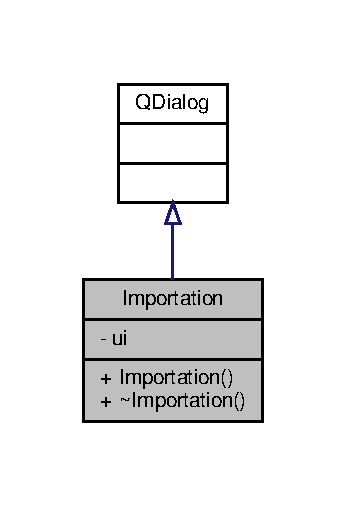
\includegraphics[width=166pt]{class_importation__coll__graph}
\end{center}
\end{figure}
\subsubsection*{Fonctions membres publiques}
\begin{DoxyCompactItemize}
\item 
\hyperlink{class_importation_ad3a625fb90d559ff048151a4cb4646b4}{Importation} (\hyperlink{class_q_widget}{Q\+Widget} $\ast$parent=nullptr)
\begin{DoxyCompactList}\small\item\em Constructeur de la classe \hyperlink{class_importation}{Importation}. \end{DoxyCompactList}\item 
\hyperlink{class_importation_ac9f6f0a390369d5732576fb38a8e62c7}{$\sim$\+Importation} ()
\begin{DoxyCompactList}\small\item\em Destructeur de la classe \hyperlink{class_importation}{Importation}. \end{DoxyCompactList}\end{DoxyCompactItemize}
\subsubsection*{Attributs privés}
\begin{DoxyCompactItemize}
\item 
Ui\+::\+Importation $\ast$ \hyperlink{class_importation_ace5d522c27957bac47fd8d3234af1d2e}{ui}
\end{DoxyCompactItemize}


\subsubsection{Description détaillée}
Classe permetant de d\textquotesingle{}importer le calendrier. 

Définition à la ligne \hyperlink{importation_8h_source_l00017}{17} du fichier \hyperlink{importation_8h_source}{importation.\+h}.



\subsubsection{Documentation des constructeurs et destructeur}
\mbox{\Hypertarget{class_importation_ad3a625fb90d559ff048151a4cb4646b4}\label{class_importation_ad3a625fb90d559ff048151a4cb4646b4}} 
\index{Importation@{Importation}!Importation@{Importation}}
\index{Importation@{Importation}!Importation@{Importation}}
\paragraph{\texorpdfstring{Importation()}{Importation()}}
{\footnotesize\ttfamily Importation\+::\+Importation (\begin{DoxyParamCaption}\item[{\hyperlink{class_q_widget}{Q\+Widget} $\ast$}]{parent = {\ttfamily nullptr} }\end{DoxyParamCaption})\hspace{0.3cm}{\ttfamily [explicit]}}



Constructeur de la classe \hyperlink{class_importation}{Importation}. 


\begin{DoxyParams}{Paramètres}
{\em parent} & \\
\hline
\end{DoxyParams}


Définition à la ligne \hyperlink{importation_8cpp_source_l00004}{4} du fichier \hyperlink{importation_8cpp_source}{importation.\+cpp}.



Références \hyperlink{importation_8h_source_l00038}{ui}.


\begin{DoxyCode}
00004                                         : \hyperlink{class_q_dialog}{QDialog}(parent), \hyperlink{class_importation_ace5d522c27957bac47fd8d3234af1d2e}{ui}(\textcolor{keyword}{new} Ui::Importation)
00005 \{
00006      qDebug() << Q\_FUNC\_INFO;
00007     \hyperlink{class_importation_ace5d522c27957bac47fd8d3234af1d2e}{ui}->setupUi(\textcolor{keyword}{this});
00008 \}
\end{DoxyCode}
\mbox{\Hypertarget{class_importation_ac9f6f0a390369d5732576fb38a8e62c7}\label{class_importation_ac9f6f0a390369d5732576fb38a8e62c7}} 
\index{Importation@{Importation}!````~Importation@{$\sim$\+Importation}}
\index{````~Importation@{$\sim$\+Importation}!Importation@{Importation}}
\paragraph{\texorpdfstring{$\sim$\+Importation()}{~Importation()}}
{\footnotesize\ttfamily Importation\+::$\sim$\+Importation (\begin{DoxyParamCaption}{ }\end{DoxyParamCaption})}



Destructeur de la classe \hyperlink{class_importation}{Importation}. 


\begin{DoxyParams}{Paramètres}
{\em parent} & \\
\hline
\end{DoxyParams}


Définition à la ligne \hyperlink{importation_8cpp_source_l00010}{10} du fichier \hyperlink{importation_8cpp_source}{importation.\+cpp}.



Références \hyperlink{importation_8h_source_l00038}{ui}.


\begin{DoxyCode}
00011 \{
00012     \textcolor{keyword}{delete} \hyperlink{class_importation_ace5d522c27957bac47fd8d3234af1d2e}{ui};
00013     qDebug() << Q\_FUNC\_INFO;
00014 \}
\end{DoxyCode}


\subsubsection{Documentation des données membres}
\mbox{\Hypertarget{class_importation_ace5d522c27957bac47fd8d3234af1d2e}\label{class_importation_ace5d522c27957bac47fd8d3234af1d2e}} 
\index{Importation@{Importation}!ui@{ui}}
\index{ui@{ui}!Importation@{Importation}}
\paragraph{\texorpdfstring{ui}{ui}}
{\footnotesize\ttfamily Ui\+::\+Importation$\ast$ Importation\+::ui\hspace{0.3cm}{\ttfamily [private]}}



Définition à la ligne \hyperlink{importation_8h_source_l00038}{38} du fichier \hyperlink{importation_8h_source}{importation.\+h}.



Référencé par \hyperlink{importation_8cpp_source_l00004}{Importation()}, et \hyperlink{importation_8cpp_source_l00010}{$\sim$\+Importation()}.



La documentation de cette classe a été générée à partir des fichiers suivants \+:\begin{DoxyCompactItemize}
\item 
\hyperlink{importation_8h}{importation.\+h}\item 
\hyperlink{importation_8cpp}{importation.\+cpp}\end{DoxyCompactItemize}

\hypertarget{class_message_personnalise}{}\subsection{Référence de la classe Message\+Personnalise}
\label{class_message_personnalise}\index{Message\+Personnalise@{Message\+Personnalise}}


Classe permetant de personnalisé son message.  




{\ttfamily \#include \char`\"{}messagepersonnalise.\+h\char`\"{}}



Graphe de collaboration de Message\+Personnalise\+:
\nopagebreak
\begin{figure}[H]
\begin{center}
\leavevmode
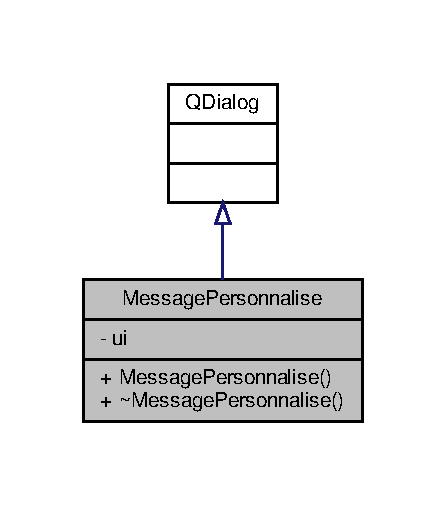
\includegraphics[width=214pt]{class_message_personnalise__coll__graph}
\end{center}
\end{figure}
\subsubsection*{Fonctions membres publiques}
\begin{DoxyCompactItemize}
\item 
\hyperlink{class_message_personnalise_ac36a9573287d1119566790a4fad25dbc}{Message\+Personnalise} (\hyperlink{class_q_widget}{Q\+Widget} $\ast$parent=nullptr)
\begin{DoxyCompactList}\small\item\em Constructeur de la classe \hyperlink{class_message_personnalise}{Message\+Personnalise}. \end{DoxyCompactList}\item 
\hyperlink{class_message_personnalise_aff9181649ac956114f02660582e86cfc}{$\sim$\+Message\+Personnalise} ()
\begin{DoxyCompactList}\small\item\em Destructeur de la classe \hyperlink{class_message_personnalise}{Message\+Personnalise}. \end{DoxyCompactList}\end{DoxyCompactItemize}
\subsubsection*{Attributs privés}
\begin{DoxyCompactItemize}
\item 
Ui\+::\+Message\+Personnalise $\ast$ \hyperlink{class_message_personnalise_a94bdf252f3e858ec1c2ed354d31a91e3}{ui}
\end{DoxyCompactItemize}


\subsubsection{Description détaillée}
Classe permetant de personnalisé son message. 

Définition à la ligne \hyperlink{messagepersonnalise_8h_source_l00016}{16} du fichier \hyperlink{messagepersonnalise_8h_source}{messagepersonnalise.\+h}.



\subsubsection{Documentation des constructeurs et destructeur}
\mbox{\Hypertarget{class_message_personnalise_ac36a9573287d1119566790a4fad25dbc}\label{class_message_personnalise_ac36a9573287d1119566790a4fad25dbc}} 
\index{Message\+Personnalise@{Message\+Personnalise}!Message\+Personnalise@{Message\+Personnalise}}
\index{Message\+Personnalise@{Message\+Personnalise}!Message\+Personnalise@{Message\+Personnalise}}
\paragraph{\texorpdfstring{Message\+Personnalise()}{MessagePersonnalise()}}
{\footnotesize\ttfamily Message\+Personnalise\+::\+Message\+Personnalise (\begin{DoxyParamCaption}\item[{\hyperlink{class_q_widget}{Q\+Widget} $\ast$}]{parent = {\ttfamily nullptr} }\end{DoxyParamCaption})\hspace{0.3cm}{\ttfamily [explicit]}}



Constructeur de la classe \hyperlink{class_message_personnalise}{Message\+Personnalise}. 


\begin{DoxyParams}{Paramètres}
{\em parent} & \\
\hline
\end{DoxyParams}


Définition à la ligne \hyperlink{messagepersonnalise_8cpp_source_l00004}{4} du fichier \hyperlink{messagepersonnalise_8cpp_source}{messagepersonnalise.\+cpp}.



Références \hyperlink{messagepersonnalise_8h_source_l00037}{ui}.


\begin{DoxyCode}
00004                                                         :
00005     \hyperlink{class_q_dialog}{QDialog}(parent),
00006     \hyperlink{class_message_personnalise_a94bdf252f3e858ec1c2ed354d31a91e3}{ui}(\textcolor{keyword}{new} Ui::MessagePersonnalise)
00007 \{
00008      qDebug() << Q\_FUNC\_INFO;
00009     \hyperlink{class_message_personnalise_a94bdf252f3e858ec1c2ed354d31a91e3}{ui}->setupUi(\textcolor{keyword}{this});
00010 \}
\end{DoxyCode}
\mbox{\Hypertarget{class_message_personnalise_aff9181649ac956114f02660582e86cfc}\label{class_message_personnalise_aff9181649ac956114f02660582e86cfc}} 
\index{Message\+Personnalise@{Message\+Personnalise}!````~Message\+Personnalise@{$\sim$\+Message\+Personnalise}}
\index{````~Message\+Personnalise@{$\sim$\+Message\+Personnalise}!Message\+Personnalise@{Message\+Personnalise}}
\paragraph{\texorpdfstring{$\sim$\+Message\+Personnalise()}{~MessagePersonnalise()}}
{\footnotesize\ttfamily Message\+Personnalise\+::$\sim$\+Message\+Personnalise (\begin{DoxyParamCaption}{ }\end{DoxyParamCaption})}



Destructeur de la classe \hyperlink{class_message_personnalise}{Message\+Personnalise}. 


\begin{DoxyParams}{Paramètres}
{\em parent} & \\
\hline
\end{DoxyParams}


Définition à la ligne \hyperlink{messagepersonnalise_8cpp_source_l00012}{12} du fichier \hyperlink{messagepersonnalise_8cpp_source}{messagepersonnalise.\+cpp}.



Références \hyperlink{messagepersonnalise_8h_source_l00037}{ui}.


\begin{DoxyCode}
00013 \{
00014     \textcolor{keyword}{delete} \hyperlink{class_message_personnalise_a94bdf252f3e858ec1c2ed354d31a91e3}{ui};
00015     qDebug() << Q\_FUNC\_INFO;
00016 \}
\end{DoxyCode}


\subsubsection{Documentation des données membres}
\mbox{\Hypertarget{class_message_personnalise_a94bdf252f3e858ec1c2ed354d31a91e3}\label{class_message_personnalise_a94bdf252f3e858ec1c2ed354d31a91e3}} 
\index{Message\+Personnalise@{Message\+Personnalise}!ui@{ui}}
\index{ui@{ui}!Message\+Personnalise@{Message\+Personnalise}}
\paragraph{\texorpdfstring{ui}{ui}}
{\footnotesize\ttfamily Ui\+::\+Message\+Personnalise$\ast$ Message\+Personnalise\+::ui\hspace{0.3cm}{\ttfamily [private]}}



Définition à la ligne \hyperlink{messagepersonnalise_8h_source_l00037}{37} du fichier \hyperlink{messagepersonnalise_8h_source}{messagepersonnalise.\+h}.



Référencé par \hyperlink{messagepersonnalise_8cpp_source_l00004}{Message\+Personnalise()}, et \hyperlink{messagepersonnalise_8cpp_source_l00012}{$\sim$\+Message\+Personnalise()}.



La documentation de cette classe a été générée à partir des fichiers suivants \+:\begin{DoxyCompactItemize}
\item 
\hyperlink{messagepersonnalise_8h}{messagepersonnalise.\+h}\item 
\hyperlink{messagepersonnalise_8cpp}{messagepersonnalise.\+cpp}\end{DoxyCompactItemize}

\hypertarget{class_q_dialog}{}\subsection{Référence de la classe Q\+Dialog}
\label{class_q_dialog}\index{Q\+Dialog@{Q\+Dialog}}


Graphe de collaboration de Q\+Dialog\+:
\nopagebreak
\begin{figure}[H]
\begin{center}
\leavevmode
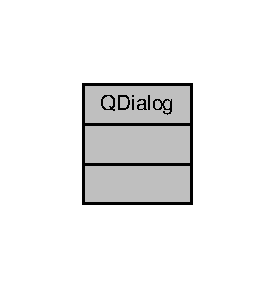
\includegraphics[width=132pt]{class_q_dialog__coll__graph}
\end{center}
\end{figure}


La documentation de cette classe a été générée à partir du fichier suivant \+:\begin{DoxyCompactItemize}
\item 
\hyperlink{messagepersonnalise_8h}{messagepersonnalise.\+h}\end{DoxyCompactItemize}

\hypertarget{class_q_object}{}\subsection{Référence de la classe Q\+Object}
\label{class_q_object}\index{Q\+Object@{Q\+Object}}


Graphe de collaboration de Q\+Object\+:
\nopagebreak
\begin{figure}[H]
\begin{center}
\leavevmode
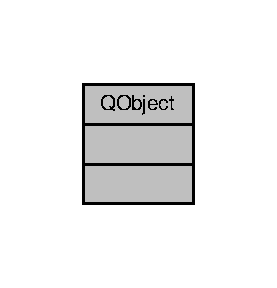
\includegraphics[width=133pt]{class_q_object__coll__graph}
\end{center}
\end{figure}


La documentation de cette classe a été générée à partir du fichier suivant \+:\begin{DoxyCompactItemize}
\item 
\hyperlink{controle_8h}{controle.\+h}\end{DoxyCompactItemize}

\hypertarget{class_q_widget}{}\subsection{Référence de la classe Q\+Widget}
\label{class_q_widget}\index{Q\+Widget@{Q\+Widget}}


Graphe de collaboration de Q\+Widget\+:
\nopagebreak
\begin{figure}[H]
\begin{center}
\leavevmode
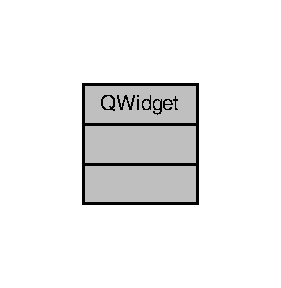
\includegraphics[width=135pt]{class_q_widget__coll__graph}
\end{center}
\end{figure}


La documentation de cette classe a été générée à partir du fichier suivant \+:\begin{DoxyCompactItemize}
\item 
\hyperlink{ihmgroom_8h}{ihmgroom.\+h}\end{DoxyCompactItemize}

\section{Documentation des fichiers}
\hypertarget{bdd_8cpp}{}\subsection{Référence du fichier bdd.\+cpp}
\label{bdd_8cpp}\index{bdd.\+cpp@{bdd.\+cpp}}
{\ttfamily \#include \char`\"{}bdd.\+h\char`\"{}}\newline
{\ttfamily \#include \char`\"{}ui\+\_\+bdd.\+h\char`\"{}}\newline

\hypertarget{bdd_8cpp_source}{}\subsection{bdd.\+cpp}

\begin{DoxyCode}
00001 \textcolor{preprocessor}{#include "\hyperlink{bdd_8h}{bdd.h}"}
00002 \textcolor{preprocessor}{#include "ui\_bdd.h"}
00003 
\Hypertarget{bdd_8cpp_source_l00004}\hyperlink{class_bdd_a9b439e0eaab93fcea818892e1daf809b}{00004} \hyperlink{class_bdd_a9b439e0eaab93fcea818892e1daf809b}{Bdd::Bdd}(\hyperlink{class_q_widget}{QWidget} *parent) :
00005     \hyperlink{class_q_dialog}{QDialog}(parent),
00006     ui(new \hyperlink{namespace_ui}{Ui}::\hyperlink{class_bdd}{Bdd})
00007 \{
00008     \hyperlink{class_bdd_a7d9f43a44caaddb2f5ccd728ecc78c2a}{ui}->setupUi(\textcolor{keyword}{this});
00009 \}
00010 
\Hypertarget{bdd_8cpp_source_l00011}\hyperlink{class_bdd_a5029277f27f8cfcf9d8603fb331a15dd}{00011} \hyperlink{class_bdd_a5029277f27f8cfcf9d8603fb331a15dd}{Bdd::~Bdd}()
00012 \{
00013     \textcolor{keyword}{delete} \hyperlink{class_bdd_a7d9f43a44caaddb2f5ccd728ecc78c2a}{ui};
00014 \}
\end{DoxyCode}

\hypertarget{bdd_8h}{}\subsection{Référence du fichier bdd.\+h}
\label{bdd_8h}\index{bdd.\+h@{bdd.\+h}}
{\ttfamily \#include $<$Qt\+Widgets$>$}\newline
\subsubsection*{Classes}
\begin{DoxyCompactItemize}
\item 
class \hyperlink{class_bdd}{Bdd}
\end{DoxyCompactItemize}
\subsubsection*{Espaces de nommage}
\begin{DoxyCompactItemize}
\item 
 \hyperlink{namespace_ui}{Ui}
\end{DoxyCompactItemize}

\hypertarget{bdd_8h_source}{}\subsection{bdd.\+h}

\begin{DoxyCode}
00001 \textcolor{preprocessor}{#ifndef BDD\_H}
00002 \textcolor{preprocessor}{#define BDD\_H}
00003 
00004 \textcolor{preprocessor}{#include <QtWidgets>}
00005 
\Hypertarget{bdd_8h_source_l00006}\hyperlink{namespace_ui}{00006} \textcolor{keyword}{namespace }\hyperlink{namespace_ui}{Ui} \{
00007 \textcolor{keyword}{class }\hyperlink{class_bdd}{Bdd};
00008 \}
00009 
\Hypertarget{bdd_8h_source_l00010}\hyperlink{class_bdd}{00010} \textcolor{keyword}{class }\hyperlink{class_bdd}{Bdd} : \textcolor{keyword}{public} \hyperlink{class_q_dialog}{QDialog}
00011 \{
00012     Q\_OBJECT
00013 
00014 \textcolor{keyword}{public}:
00015     \textcolor{keyword}{explicit} \hyperlink{class_bdd}{Bdd}(\hyperlink{class_q_widget}{QWidget} *parent = \textcolor{keyword}{nullptr});
00016     ~\hyperlink{class_bdd}{Bdd}();
00017 
00018 \textcolor{keyword}{private}:
\Hypertarget{bdd_8h_source_l00019}\hyperlink{class_bdd_a7d9f43a44caaddb2f5ccd728ecc78c2a}{00019}     Ui::Bdd *\hyperlink{class_bdd_a7d9f43a44caaddb2f5ccd728ecc78c2a}{ui};
00020 \};
00021 
00022 \textcolor{preprocessor}{#endif // BDD\_H}
\end{DoxyCode}

\hypertarget{_changelog_8md}{}\subsection{Référence du fichier Changelog.\+md}
\label{_changelog_8md}\index{Changelog.\+md@{Changelog.\+md}}

\hypertarget{_changelog_8md_source}{}\subsection{Changelog.\+md}

\begin{DoxyCode}
00001 \(\backslash\)page page\_changelog Changelog
00002 
00003 r1 | www-data | 2020-02-01 15:03:29 +0100 (sam. 01 févr. 2020) | 1 ligne
00004 
00005 Creating initial repository structure
\end{DoxyCode}

\hypertarget{communicationbluetooth_8cpp}{}\subsection{Référence du fichier communicationbluetooth.\+cpp}
\label{communicationbluetooth_8cpp}\index{communicationbluetooth.\+cpp@{communicationbluetooth.\+cpp}}
{\ttfamily \#include \char`\"{}communicationbluetooth.\+h\char`\"{}}\newline
{\ttfamily \#include \char`\"{}ui\+\_\+communicationbluetooth.\+h\char`\"{}}\newline

\hypertarget{communicationbluetooth_8cpp_source}{}\subsection{communicationbluetooth.\+cpp}

\begin{DoxyCode}
00001 \textcolor{preprocessor}{#include "\hyperlink{communicationbluetooth_8h}{communicationbluetooth.h}"}
00002 \textcolor{preprocessor}{#include "ui\_communicationbluetooth.h"}
00003 
\Hypertarget{communicationbluetooth_8cpp_source_l00004}\hyperlink{class_communication_bluetooth_a30f88d1710eb41d9c8c4b390b5c7b6f7}{00004} \hyperlink{class_communication_bluetooth_a30f88d1710eb41d9c8c4b390b5c7b6f7}{CommunicationBluetooth::CommunicationBluetooth}(
      \hyperlink{class_q_widget}{QWidget} *parent) :
00005     \hyperlink{class_q_dialog}{QDialog}(parent),
00006     ui(new \hyperlink{namespace_ui}{Ui}::\hyperlink{class_communication_bluetooth}{CommunicationBluetooth})
00007 \{
00008      qDebug() << Q\_FUNC\_INFO;
00009     \hyperlink{class_communication_bluetooth_a2721cf9f9503a98770981ffdad09f9a1}{ui}->setupUi(\textcolor{keyword}{this});
00010 \}
00011 
\Hypertarget{communicationbluetooth_8cpp_source_l00012}\hyperlink{class_communication_bluetooth_a13c72d24359f40c204e94f3ef1ab6fd3}{00012} \hyperlink{class_communication_bluetooth_a13c72d24359f40c204e94f3ef1ab6fd3}{CommunicationBluetooth::~CommunicationBluetooth}()
00013 \{
00014     \textcolor{keyword}{delete} \hyperlink{class_communication_bluetooth_a2721cf9f9503a98770981ffdad09f9a1}{ui};
00015     qDebug() << Q\_FUNC\_INFO;
00016 \}
\end{DoxyCode}

\hypertarget{communicationbluetooth_8h}{}\subsection{Référence du fichier communicationbluetooth.\+h}
\label{communicationbluetooth_8h}\index{communicationbluetooth.\+h@{communicationbluetooth.\+h}}
{\ttfamily \#include $<$Qt\+Widgets$>$}\newline
\subsubsection*{Classes}
\begin{DoxyCompactItemize}
\item 
class \hyperlink{class_communication_bluetooth}{Communication\+Bluetooth}
\begin{DoxyCompactList}\small\item\em Class permettant de mettre en place une communication bluetooth. \end{DoxyCompactList}\end{DoxyCompactItemize}
\subsubsection*{Espaces de nommage}
\begin{DoxyCompactItemize}
\item 
 \hyperlink{namespace_ui}{Ui}
\end{DoxyCompactItemize}

\hypertarget{communicationbluetooth_8h_source}{}\subsection{communicationbluetooth.\+h}

\begin{DoxyCode}
00001 \textcolor{preprocessor}{#ifndef COMMUNICATIONBLUETOOTH\_H}
00002 \textcolor{preprocessor}{#define COMMUNICATIONBLUETOOTH\_H}
00003 
00004 \textcolor{preprocessor}{#include <QtWidgets>}
00005 
00006 
00012 \textcolor{keyword}{class }\hyperlink{class_ihm_groom}{IhmGroom};
00013 \textcolor{keyword}{namespace }\hyperlink{namespace_ui}{Ui} \{
00014 \textcolor{keyword}{class }\hyperlink{class_communication_bluetooth}{CommunicationBluetooth};
00015 \}
00016 
\Hypertarget{communicationbluetooth_8h_source_l00017}\hyperlink{class_communication_bluetooth}{00017} \textcolor{keyword}{class }\hyperlink{class_communication_bluetooth}{CommunicationBluetooth} : \textcolor{keyword}{public} \hyperlink{class_q_dialog}{QDialog}
00018 \{
00019     Q\_OBJECT
00020 
00021 \textcolor{keyword}{public}:
00028     \textcolor{keyword}{explicit} \hyperlink{class_communication_bluetooth}{CommunicationBluetooth}(\hyperlink{class_q_widget}{QWidget} *parent = \textcolor{keyword}{nullptr});
00035     ~\hyperlink{class_communication_bluetooth}{CommunicationBluetooth}();
00036 
00037 \textcolor{keyword}{private}:
\Hypertarget{communicationbluetooth_8h_source_l00038}\hyperlink{class_communication_bluetooth_a2721cf9f9503a98770981ffdad09f9a1}{00038}     Ui::CommunicationBluetooth *\hyperlink{class_communication_bluetooth_a2721cf9f9503a98770981ffdad09f9a1}{ui}; 
00039 \};
00040 
00041 \textcolor{preprocessor}{#endif // COMMUNICATIONBLUETOOTH\_H}
\end{DoxyCode}

\hypertarget{controle_8cpp}{}\subsection{Référence du fichier controle.\+cpp}
\label{controle_8cpp}\index{controle.\+cpp@{controle.\+cpp}}
{\ttfamily \#include \char`\"{}controle.\+h\char`\"{}}\newline
{\ttfamily \#include $<$Q\+Debug$>$}\newline

\hypertarget{controle_8cpp_source}{}\subsection{controle.\+cpp}

\begin{DoxyCode}
00001 \textcolor{preprocessor}{#include "\hyperlink{controle_8h}{controle.h}"}
00002 \textcolor{preprocessor}{#include <QDebug>}
00003 
00004 
\Hypertarget{controle_8cpp_source_l00005}\hyperlink{class_controle_af64a33acc664bf02f2ea0b4f27f781e6}{00005} \hyperlink{class_controle_af64a33acc664bf02f2ea0b4f27f781e6}{Controle::Controle}(\hyperlink{class_q_object}{QObject} *parent) : \hyperlink{class_q_object}{QObject}(parent)
00006 \{
00007      qDebug() << Q\_FUNC\_INFO;
00008    \textcolor{comment}{//     ui = new IhmGroom;}
00009     \hyperlink{class_controle_afddf1dce812ff88577e308684b564f33}{etatSonnette} = \textcolor{keyword}{true};
00010 
00011 \}
00012 
\Hypertarget{controle_8cpp_source_l00013}\hyperlink{class_controle_a98f5d2630efbdb5f469cbb2675725b20}{00013} \hyperlink{class_controle_a98f5d2630efbdb5f469cbb2675725b20}{Controle::~Controle}()
00014 \{
00015     qDebug() << Q\_FUNC\_INFO;
00016 \}
00017 
\Hypertarget{controle_8cpp_source_l00018}\hyperlink{class_controle_a62db54114d126d03dd332332b3942320}{00018} \textcolor{keywordtype}{void} \hyperlink{class_controle_a62db54114d126d03dd332332b3942320}{Controle::setEtatUtilisateur}(\textcolor{keywordtype}{int} newEtatUtilisateur)
00019 \{
00020     \hyperlink{class_controle_a690595803de8f5c172b8bc46122ebb1a}{etatUtilisateur} = newEtatUtilisateur;
00021 \}
00022 
\Hypertarget{controle_8cpp_source_l00023}\hyperlink{class_controle_ac3bd8e8621cee56d4343e21a624e1c48}{00023} \textcolor{keywordtype}{int} \hyperlink{class_controle_ac3bd8e8621cee56d4343e21a624e1c48}{Controle::getEtatUtilisateur}()
00024 \{
00025     \textcolor{keywordflow}{return} \hyperlink{class_controle_a690595803de8f5c172b8bc46122ebb1a}{etatUtilisateur};
00026 \}
00027 
\Hypertarget{controle_8cpp_source_l00028}\hyperlink{class_controle_ac706c5e9ede46dab70631281b084e233}{00028} \textcolor{keywordtype}{void} \hyperlink{class_controle_ac706c5e9ede46dab70631281b084e233}{Controle::setEtatSonnette}(\textcolor{keywordtype}{bool} newEtatSonnette)
00029 \{
00030     \hyperlink{class_controle_afddf1dce812ff88577e308684b564f33}{etatSonnette} = newEtatSonnette;
00031 \}
00032 
\Hypertarget{controle_8cpp_source_l00033}\hyperlink{class_controle_acabf3768430c7f1acb268ca0fa1ddf99}{00033} \textcolor{keywordtype}{bool} \hyperlink{class_controle_acabf3768430c7f1acb268ca0fa1ddf99}{Controle::getEtatSonnette}()
00034 \{
00035     \textcolor{keywordflow}{return} \hyperlink{class_controle_afddf1dce812ff88577e308684b564f33}{etatSonnette};
00036 \}
00037 
\Hypertarget{controle_8cpp_source_l00038}\hyperlink{class_controle_a65904fe693663759a4cde4e4d66e36e8}{00038} \textcolor{keywordtype}{void} \hyperlink{class_controle_a65904fe693663759a4cde4e4d66e36e8}{Controle::setPresence}(\textcolor{keywordtype}{bool} newPresence)
00039 \{
00040     \hyperlink{class_controle_a089f74f48f24f09e7fc51b03a5ede79e}{presence} = newPresence;
00041 \}
00042 
\Hypertarget{controle_8cpp_source_l00043}\hyperlink{class_controle_abf7c9fefec4980b90c9f759d48fd17aa}{00043} \textcolor{keywordtype}{bool} \hyperlink{class_controle_abf7c9fefec4980b90c9f759d48fd17aa}{Controle::getPresence}()
00044 \{
00045     \textcolor{keywordflow}{return} \hyperlink{class_controle_a089f74f48f24f09e7fc51b03a5ede79e}{presence};
00046 \}
00047 
00048 
\Hypertarget{controle_8cpp_source_l00049}\hyperlink{class_controle_a2dcdd01e67e6ce8769188d62ce0c262a}{00049} \textcolor{keywordtype}{void} \hyperlink{class_controle_a2dcdd01e67e6ce8769188d62ce0c262a}{Controle::decoderTrameGroom}(QString \hyperlink{class_controle_a5b9512ebbaf16746f55a9519de88f9be}{trameGroom})
00050 \{
00051 
00052     \hyperlink{class_controle_a62db54114d126d03dd332332b3942320}{setEtatUtilisateur}((trameGroom.section(\textcolor{stringliteral}{";"},1,1)).toInt());
00053 
00054 
00055     \textcolor{keywordflow}{if} (trameGroom.section(\textcolor{stringliteral}{";"},2,2) == 1)
00056     \{
00057         \hyperlink{class_controle_ac706c5e9ede46dab70631281b084e233}{setEtatSonnette}(\textcolor{keyword}{true});
00058     \}
00059     \textcolor{keywordflow}{else}
00060     \{
00061         \hyperlink{class_controle_ac706c5e9ede46dab70631281b084e233}{setEtatSonnette}(\textcolor{keyword}{false});
00062     \}
00063 
00064     \textcolor{keywordflow}{if} (trameGroom.section(\textcolor{stringliteral}{";"},3,3) == 1)
00065     \{
00066         \hyperlink{class_controle_a65904fe693663759a4cde4e4d66e36e8}{setPresence}(\textcolor{keyword}{true});
00067     \}
00068     \textcolor{keywordflow}{else}
00069     \{
00070         \hyperlink{class_controle_a65904fe693663759a4cde4e4d66e36e8}{setPresence}(\textcolor{keyword}{false});
00071     \}
00072 
00073 \}
00074 
\Hypertarget{controle_8cpp_source_l00075}\hyperlink{class_controle_a0f731cdb733053f7be24e7042611601c}{00075} \textcolor{keywordtype}{void} \hyperlink{class_controle_a0f731cdb733053f7be24e7042611601c}{Controle::setNom}(QString newNom)
00076 \{
00077     \hyperlink{class_controle_ad47747a49ca21434f6d43d451d3cf134}{nom} = newNom;
00078 \}
00079 
\Hypertarget{controle_8cpp_source_l00080}\hyperlink{class_controle_ac6e8590a5108e97fce3ce3aa43feb881}{00080} QString \hyperlink{class_controle_ac6e8590a5108e97fce3ce3aa43feb881}{Controle::getNom}()
00081 \{
00082     \textcolor{keywordflow}{return} \hyperlink{class_controle_ad47747a49ca21434f6d43d451d3cf134}{nom};
00083 \}
\Hypertarget{controle_8cpp_source_l00084}\hyperlink{class_controle_ab046adc050872b4034c1500eb2e1b728}{00084} \textcolor{keywordtype}{void} \hyperlink{class_controle_ab046adc050872b4034c1500eb2e1b728}{Controle::setPrenom}(QString newPrenom)
00085 \{
00086     \hyperlink{class_controle_a29e37e25a6fd4643ddea3fef47e3bc51}{prenom} = newPrenom;
00087 \}
\Hypertarget{controle_8cpp_source_l00088}\hyperlink{class_controle_a0164fd9066b1703498576095ab5642c5}{00088} QString \hyperlink{class_controle_a0164fd9066b1703498576095ab5642c5}{Controle::getPrenom}()
00089 \{
00090     \textcolor{keywordflow}{return} \hyperlink{class_controle_a29e37e25a6fd4643ddea3fef47e3bc51}{prenom};
00091 \}
\Hypertarget{controle_8cpp_source_l00092}\hyperlink{class_controle_abe472f4fd197c0fc679539e0b75a6e15}{00092} \textcolor{keywordtype}{void} \hyperlink{class_controle_abe472f4fd197c0fc679539e0b75a6e15}{Controle::setFonction}(QString newFonction)
00093 \{
00094     \hyperlink{class_controle_af733c06309ce63fb9157073574e42b00}{fonction} = newFonction;
00095 \}
\Hypertarget{controle_8cpp_source_l00096}\hyperlink{class_controle_a8d2891b2b01c503d10f775b4b14a3777}{00096} QString \hyperlink{class_controle_a8d2891b2b01c503d10f775b4b14a3777}{Controle::getFonction}()
00097 \{
00098     \textcolor{keywordflow}{return} \hyperlink{class_controle_af733c06309ce63fb9157073574e42b00}{fonction};
00099 \}
00100 
\Hypertarget{controle_8cpp_source_l00101}\hyperlink{class_controle_a316808279226b01ac8fe51ab396b1b67}{00101} \textcolor{keywordtype}{void} \hyperlink{class_controle_a316808279226b01ac8fe51ab396b1b67}{Controle::coderTrameAffichage}(QString 
      \hyperlink{class_controle_a0bbdd7a0c44fbbc45bf3a381872fcfbe}{trameAffichage})
00102 \{
00103     \hyperlink{class_controle_a0f731cdb733053f7be24e7042611601c}{setNom}(trameAffichage.section(\textcolor{stringliteral}{";"},1,1));
00104 
00105     \hyperlink{class_controle_ab046adc050872b4034c1500eb2e1b728}{setPrenom}(trameAffichage.section(\textcolor{stringliteral}{";"},2,2));
00106 
00107     \hyperlink{class_controle_abe472f4fd197c0fc679539e0b75a6e15}{setFonction}(trameAffichage.section(\textcolor{stringliteral}{";"},3,3));
00108 
00109     \hyperlink{class_controle_a2dd60c955396dd80426c1a74f56ea611}{ui}->\hyperlink{class_ihm_groom_aa270d1fb6a7a9c1385c4ae3e67451ea0}{changementNom}();
00110     \hyperlink{class_controle_a2dd60c955396dd80426c1a74f56ea611}{ui}->\hyperlink{class_ihm_groom_a2e8db190224f15326552a5bd642a9347}{changementPrenom}();
00111     \hyperlink{class_controle_a2dd60c955396dd80426c1a74f56ea611}{ui}->\hyperlink{class_ihm_groom_afc6c48489b270b22a660e32668d6b2ca}{changementFonction}();
00112 \}
\end{DoxyCode}

\hypertarget{controle_8h}{}\subsection{Référence du fichier controle.\+h}
\label{controle_8h}\index{controle.\+h@{controle.\+h}}
{\ttfamily \#include $<$Q\+Object$>$}\newline
{\ttfamily \#include $<$Q\+Date\+Time$>$}\newline
{\ttfamily \#include $<$Q\+String$>$}\newline
{\ttfamily \#include \char`\"{}communicationbluetooth.\+h\char`\"{}}\newline
{\ttfamily \#include \char`\"{}ihmgroom.\+h\char`\"{}}\newline
{\ttfamily \#include \char`\"{}messagepersonnalise.\+h\char`\"{}}\newline
\subsubsection*{Classes}
\begin{DoxyCompactItemize}
\item 
class \hyperlink{class_controle}{Controle}
\begin{DoxyCompactList}\small\item\em Classe assurant le controle et la validé de l\textquotesingle{}envoie et réception des trames. \end{DoxyCompactList}\end{DoxyCompactItemize}

\hypertarget{controle_8h_source}{}\subsection{controle.\+h}

\begin{DoxyCode}
00001 \textcolor{preprocessor}{#ifndef CONTROLE\_H}
00002 \textcolor{preprocessor}{#define CONTROLE\_H}
00003 
00004 \textcolor{preprocessor}{#include <QObject>}
00005 \textcolor{preprocessor}{#include <QDateTime>}
00006 \textcolor{preprocessor}{#include <QString>}
00007 \textcolor{preprocessor}{#include "\hyperlink{communicationbluetooth_8h}{communicationbluetooth.h}"}
00008 \textcolor{preprocessor}{#include "\hyperlink{ihmgroom_8h}{ihmgroom.h}"}
00009 \textcolor{preprocessor}{#include "\hyperlink{messagepersonnalise_8h}{messagepersonnalise.h}"}
00010 
00017 \textcolor{keyword}{class }\hyperlink{class_ihm_groom}{IhmGroom};
00018 \textcolor{keyword}{class }\hyperlink{class_communication_bluetooth}{CommunicationBluetooth};
00019 \textcolor{keyword}{class }\hyperlink{class_message_personnalise}{MessagePersonnalise};
00020 
00021 
\Hypertarget{controle_8h_source_l00022}\hyperlink{class_controle}{00022} \textcolor{keyword}{class }\hyperlink{class_controle}{Controle} : \textcolor{keyword}{public} \hyperlink{class_q_object}{QObject}
00023 \{
00024     Q\_OBJECT
00025 
00026     \textcolor{keyword}{private}:
\Hypertarget{controle_8h_source_l00027}\hyperlink{class_controle_a5d818564000173732472eb9ac20e53aa}{00027}         \hyperlink{class_communication_bluetooth}{CommunicationBluetooth} *\hyperlink{class_controle_a5d818564000173732472eb9ac20e53aa}{communicationBluetooth};     
\Hypertarget{controle_8h_source_l00028}\hyperlink{class_controle_a6240fc19c937146243bcd950e5408481}{00028}         \hyperlink{class_message_personnalise}{MessagePersonnalise} *\hyperlink{class_controle_a6240fc19c937146243bcd950e5408481}{messagePersonnalise};           
\Hypertarget{controle_8h_source_l00029}\hyperlink{class_controle_a2dd60c955396dd80426c1a74f56ea611}{00029}         \hyperlink{class_ihm_groom}{IhmGroom} *\hyperlink{class_controle_a2dd60c955396dd80426c1a74f56ea611}{ui};                                       
\Hypertarget{controle_8h_source_l00031}\hyperlink{class_controle_a5b9512ebbaf16746f55a9519de88f9be}{00031}         QString \hyperlink{class_controle_a5b9512ebbaf16746f55a9519de88f9be}{trameGroom};                                 
\Hypertarget{controle_8h_source_l00032}\hyperlink{class_controle_a0bbdd7a0c44fbbc45bf3a381872fcfbe}{00032}         QString \hyperlink{class_controle_a0bbdd7a0c44fbbc45bf3a381872fcfbe}{trameAffichage};                             
\Hypertarget{controle_8h_source_l00033}\hyperlink{class_controle_a5cb6dbeb8b2f066b1e757f3c933ea503}{00033}         QString \hyperlink{class_controle_a5cb6dbeb8b2f066b1e757f3c933ea503}{trameMsgPerso};                              
00042         \textcolor{keywordtype}{bool} \hyperlink{class_controle_a4f40023a18e4e656282a15d5657e0a25}{verifierChecksum}(QString trameGroom);
00048         \textcolor{keywordtype}{void} \hyperlink{class_controle_a2dcdd01e67e6ce8769188d62ce0c262a}{decoderTrameGroom}(QString trameGroom);
00054         \textcolor{keywordtype}{void} \hyperlink{class_controle_a9ba8efd42493ffd4288537a1ace4e220}{coderTrameGroom}(QString trameGroom);
00060         \textcolor{keywordtype}{void} \hyperlink{class_controle_a316808279226b01ac8fe51ab396b1b67}{coderTrameAffichage}(QString trameAffichage);
00066         \textcolor{keywordtype}{void} \hyperlink{class_controle_a77d635484c2e6fca851d40e76f422fce}{coderTrameMsgPerso}(QString trameMsgPerso);
00067 
00068 
\Hypertarget{controle_8h_source_l00069}\hyperlink{class_controle_a690595803de8f5c172b8bc46122ebb1a}{00069}         \textcolor{keywordtype}{int} \hyperlink{class_controle_a690595803de8f5c172b8bc46122ebb1a}{etatUtilisateur};                                
\Hypertarget{controle_8h_source_l00070}\hyperlink{class_controle_afddf1dce812ff88577e308684b564f33}{00070}         \textcolor{keywordtype}{bool} \hyperlink{class_controle_afddf1dce812ff88577e308684b564f33}{etatSonnette};                                  
\Hypertarget{controle_8h_source_l00071}\hyperlink{class_controle_a089f74f48f24f09e7fc51b03a5ede79e}{00071}         \textcolor{keywordtype}{bool} \hyperlink{class_controle_a089f74f48f24f09e7fc51b03a5ede79e}{presence};                                      
\Hypertarget{controle_8h_source_l00073}\hyperlink{class_controle_ad47747a49ca21434f6d43d451d3cf134}{00073}         QString \hyperlink{class_controle_ad47747a49ca21434f6d43d451d3cf134}{nom};                                        
\Hypertarget{controle_8h_source_l00074}\hyperlink{class_controle_a29e37e25a6fd4643ddea3fef47e3bc51}{00074}         QString \hyperlink{class_controle_a29e37e25a6fd4643ddea3fef47e3bc51}{prenom};                                     
\Hypertarget{controle_8h_source_l00075}\hyperlink{class_controle_af733c06309ce63fb9157073574e42b00}{00075}         QString \hyperlink{class_controle_af733c06309ce63fb9157073574e42b00}{fonction};                                   
00079     \textcolor{keyword}{public}:
00086         \hyperlink{class_controle_af64a33acc664bf02f2ea0b4f27f781e6}{Controle}(\hyperlink{class_q_object}{QObject} *parent = \textcolor{keyword}{nullptr});
00093         \hyperlink{class_controle_a98f5d2630efbdb5f469cbb2675725b20}{~Controle}();
00100         \textcolor{keywordtype}{void} \hyperlink{class_controle_ac706c5e9ede46dab70631281b084e233}{setEtatSonnette}(\textcolor{keywordtype}{bool} newEtatSonnette);
00107         \textcolor{keywordtype}{bool} \hyperlink{class_controle_acabf3768430c7f1acb268ca0fa1ddf99}{getEtatSonnette}();
00114         \textcolor{keywordtype}{void} \hyperlink{class_controle_a62db54114d126d03dd332332b3942320}{setEtatUtilisateur}(\textcolor{keywordtype}{int} newEtatUtilisateur);
00121         \textcolor{keywordtype}{int} \hyperlink{class_controle_ac3bd8e8621cee56d4343e21a624e1c48}{getEtatUtilisateur}();
00128         \textcolor{keywordtype}{void} \hyperlink{class_controle_a65904fe693663759a4cde4e4d66e36e8}{setPresence}(\textcolor{keywordtype}{bool} newPresence);
00135         \textcolor{keywordtype}{bool} \hyperlink{class_controle_abf7c9fefec4980b90c9f759d48fd17aa}{getPresence}();
00136 
00143         \textcolor{keywordtype}{void} \hyperlink{class_controle_a0f731cdb733053f7be24e7042611601c}{setNom}(QString newNom);
00150         QString \hyperlink{class_controle_ac6e8590a5108e97fce3ce3aa43feb881}{getNom}();
00157         \textcolor{keywordtype}{void} \hyperlink{class_controle_ab046adc050872b4034c1500eb2e1b728}{setPrenom}(QString newPrenom);
00164         QString \hyperlink{class_controle_a0164fd9066b1703498576095ab5642c5}{getPrenom}();
00171         \textcolor{keywordtype}{void} \hyperlink{class_controle_abe472f4fd197c0fc679539e0b75a6e15}{setFonction}(QString newFonction);
00178         QString \hyperlink{class_controle_a8d2891b2b01c503d10f775b4b14a3777}{getFonction}();
00179 
00180 
00181     \textcolor{keyword}{public} slots:
00182 
00183 \};
00184 
00185 \textcolor{preprocessor}{#endif // CONTROLE\_H}
\end{DoxyCode}

\hypertarget{ihmgroom_8cpp}{}\subsection{Référence du fichier ihmgroom.\+cpp}
\label{ihmgroom_8cpp}\index{ihmgroom.\+cpp@{ihmgroom.\+cpp}}


Définition de la classe \hyperlink{class_ihm_groom}{Ihm\+Groom}.  


{\ttfamily \#include \char`\"{}ihmgroom.\+h\char`\"{}}\newline
{\ttfamily \#include \char`\"{}ui\+\_\+ihmgroom.\+h\char`\"{}}\newline
{\ttfamily \#include \char`\"{}communicationbluetooth.\+h\char`\"{}}\newline
{\ttfamily \#include \char`\"{}ui\+\_\+communicationbluetooth.\+h\char`\"{}}\newline
{\ttfamily \#include \char`\"{}importation.\+h\char`\"{}}\newline
{\ttfamily \#include \char`\"{}ui\+\_\+importation.\+h\char`\"{}}\newline
{\ttfamily \#include \char`\"{}messagepersonnalise.\+h\char`\"{}}\newline
{\ttfamily \#include \char`\"{}ui\+\_\+messagepersonnalise.\+h\char`\"{}}\newline
{\ttfamily \#include \char`\"{}controle.\+h\char`\"{}}\newline
{\ttfamily \#include \char`\"{}bdd.\+h\char`\"{}}\newline
{\ttfamily \#include \char`\"{}ui\+\_\+bdd.\+h\char`\"{}}\newline


\subsubsection{Description détaillée}
Définition de la classe \hyperlink{class_ihm_groom}{Ihm\+Groom}. 

\begin{DoxyAuthor}{Auteur}
Etienne Valette 
\end{DoxyAuthor}


Définition dans le fichier \hyperlink{ihmgroom_8cpp_source}{ihmgroom.\+cpp}.


\hypertarget{ihmgroom_8cpp_source}{}\subsection{ihmgroom.\+cpp}

\begin{DoxyCode}
00001 \textcolor{preprocessor}{#include "\hyperlink{ihmgroom_8h}{ihmgroom.h}"}
00002 \textcolor{preprocessor}{#include "ui\_ihmgroom.h"}
00003 \textcolor{preprocessor}{#include "\hyperlink{communicationbluetooth_8h}{communicationbluetooth.h}"}
00004 \textcolor{preprocessor}{#include "ui\_communicationbluetooth.h"}
00005 \textcolor{preprocessor}{#include "\hyperlink{importation_8h}{importation.h}"}
00006 \textcolor{preprocessor}{#include "ui\_importation.h"}
00007 \textcolor{preprocessor}{#include "\hyperlink{messagepersonnalise_8h}{messagepersonnalise.h}"}
00008 \textcolor{preprocessor}{#include "ui\_messagepersonnalise.h"}
00009 \textcolor{preprocessor}{#include "\hyperlink{controle_8h}{controle.h}"}
00010 \textcolor{preprocessor}{#include "\hyperlink{bdd_8h}{bdd.h}"}
00011 \textcolor{preprocessor}{#include "ui\_bdd.h"}
00012 
\Hypertarget{ihmgroom_8cpp_source_l00031}\hyperlink{class_ihm_groom_a44887622008d41828025e2b2ccd598a7}{00031} \hyperlink{class_ihm_groom_a44887622008d41828025e2b2ccd598a7}{IhmGroom::IhmGroom}(\hyperlink{class_q_widget}{QWidget} *parent) : \hyperlink{class_q_widget}{QWidget}(parent), ui(new 
      \hyperlink{namespace_ui}{Ui}::\hyperlink{class_ihm_groom}{IhmGroom})
00032 \{
00033     qDebug() << Q\_FUNC\_INFO;
00034     \hyperlink{class_ihm_groom_af652e1ce199213b7867e44cf589c06b8}{ui}->setupUi(\textcolor{keyword}{this});
00035     setWindowTitle(\hyperlink{ihmgroom_8h_ada54de88f03c1264af632974a72cff76}{NOM\_APP});
00036 
00037     \hyperlink{class_ihm_groom_ab3f9d16d3e20234a71b1580d70ee4959}{ihmImportation} = \textcolor{keyword}{new} \hyperlink{class_importation}{Importation}(\textcolor{keyword}{this});
00038     \hyperlink{class_ihm_groom_a529729b93d7b8d17147d3b47fe9a274d}{messagePersonnalise} = \textcolor{keyword}{new} \hyperlink{class_message_personnalise}{MessagePersonnalise}(\textcolor{keyword}{this});
00039     \hyperlink{class_ihm_groom_a8e2b551df75d8dffdfbc9beb6c3691ba}{communicationBluetooth} = \textcolor{keyword}{new} \hyperlink{class_communication_bluetooth}{CommunicationBluetooth}(\textcolor{keyword}{this});
00040     \hyperlink{class_ihm_groom_acead732c303b50a3285bd311ac8a3b4f}{controle} = \textcolor{keyword}{new} \hyperlink{class_controle}{Controle}(\textcolor{keyword}{this});
00041     \hyperlink{class_ihm_groom_aba1bfff9bc610e6a626d3af4cec266f9}{bdd} = \textcolor{keyword}{new} \hyperlink{class_bdd}{Bdd}(\textcolor{keyword}{this});
00042 
00043     \hyperlink{class_ihm_groom_addfe25c3da6ddecfbdcb5b3cf062d724}{initialiserIconeSysteme}();
00044     connect(\hyperlink{class_ihm_groom_af652e1ce199213b7867e44cf589c06b8}{ui}->pushButton\_5, SIGNAL(clicked()), \textcolor{keyword}{this}, SLOT(
      \hyperlink{class_ihm_groom_a6a7d6102f1d90172215fd4f1aae6e166}{inversionImageSonnette}()));
00048     \textcolor{comment}{// Test :}
00049     connect(\hyperlink{class_ihm_groom_af652e1ce199213b7867e44cf589c06b8}{ui}->pushButton\_7, SIGNAL(clicked()), \textcolor{keyword}{this}, SLOT(\hyperlink{class_ihm_groom_a53838a4bd054fe5c85c23eced3eacc8b}{testerNotification}()));
00050     connect(\hyperlink{class_ihm_groom_af652e1ce199213b7867e44cf589c06b8}{ui}->pushButton\_6, SIGNAL(clicked()), \textcolor{keyword}{this}, SLOT(afficherIhmConfiguration()));
00051 
00052 \}
00053 
\Hypertarget{ihmgroom_8cpp_source_l00059}\hyperlink{class_ihm_groom_a89f5e00d9a36d7162da874b2290274e0}{00059} \hyperlink{class_ihm_groom_a89f5e00d9a36d7162da874b2290274e0}{IhmGroom::~IhmGroom}()
00060 \{
00061     \textcolor{keyword}{delete} \hyperlink{class_ihm_groom_af652e1ce199213b7867e44cf589c06b8}{ui};
00062      qDebug() << Q\_FUNC\_INFO;
00063 \}
00064 
\Hypertarget{ihmgroom_8cpp_source_l00065}\hyperlink{class_ihm_groom_aa270d1fb6a7a9c1385c4ae3e67451ea0}{00065} \textcolor{keywordtype}{void} \hyperlink{class_ihm_groom_aa270d1fb6a7a9c1385c4ae3e67451ea0}{IhmGroom::changementNom}()
00066 \{
00067     \hyperlink{class_ihm_groom_af652e1ce199213b7867e44cf589c06b8}{ui}->label\_Nom->setWindowTitle(\hyperlink{class_ihm_groom_acead732c303b50a3285bd311ac8a3b4f}{controle}->\hyperlink{class_controle_ac6e8590a5108e97fce3ce3aa43feb881}{getNom}());
00068 \}
00069 
\Hypertarget{ihmgroom_8cpp_source_l00070}\hyperlink{class_ihm_groom_a2e8db190224f15326552a5bd642a9347}{00070} \textcolor{keywordtype}{void} \hyperlink{class_ihm_groom_a2e8db190224f15326552a5bd642a9347}{IhmGroom::changementPrenom}()
00071 \{
00072     \hyperlink{class_ihm_groom_af652e1ce199213b7867e44cf589c06b8}{ui}->label\_Prenom->setWindowTitle(\hyperlink{class_ihm_groom_acead732c303b50a3285bd311ac8a3b4f}{controle}->\hyperlink{class_controle_a0164fd9066b1703498576095ab5642c5}{getPrenom}());
00073 \}
00074 
\Hypertarget{ihmgroom_8cpp_source_l00075}\hyperlink{class_ihm_groom_afc6c48489b270b22a660e32668d6b2ca}{00075} \textcolor{keywordtype}{void} \hyperlink{class_ihm_groom_afc6c48489b270b22a660e32668d6b2ca}{IhmGroom::changementFonction}()
00076 \{
00077     \hyperlink{class_ihm_groom_af652e1ce199213b7867e44cf589c06b8}{ui}->label\_Fonction->setWindowTitle(\hyperlink{class_ihm_groom_acead732c303b50a3285bd311ac8a3b4f}{controle}->\hyperlink{class_controle_a8d2891b2b01c503d10f775b4b14a3777}{getFonction}());
00078 \}
00079 
00080 
\Hypertarget{ihmgroom_8cpp_source_l00087}\hyperlink{class_ihm_groom_a8063930f323ce85b679c7598742f325d}{00087} \textcolor{keywordtype}{void} \hyperlink{class_ihm_groom_a8063930f323ce85b679c7598742f325d}{IhmGroom::closeEvent}(QCloseEvent *event)
00088 \{
00089     \textcolor{keywordflow}{if} (\hyperlink{class_ihm_groom_a9ca0929cf284a9a2e3e2bc3489249919}{iconeSysteme}->isVisible())
00090     \{
00091         \textcolor{keywordflow}{if}(\hyperlink{class_ihm_groom_a95d2d2b4b3b849c1b21f234844fca056}{etatInitialIconeSysteme})
00092         \{
00093             QMessageBox::information(\textcolor{keyword}{this}, \textcolor{stringliteral}{"Groom"}, \textcolor{stringliteral}{"Le programme continue à s'éxécuter. Utiliser le menu
       Quitter pour mettre fin à l'application Groom."});
00094             \hyperlink{class_ihm_groom_a95d2d2b4b3b849c1b21f234844fca056}{etatInitialIconeSysteme} = \textcolor{keyword}{false};
00095         \}
00096         hide();
00097         \textcolor{keyword}{event}->ignore();
00098     \}
00099 \}
00100 
\Hypertarget{ihmgroom_8cpp_source_l00106}\hyperlink{class_ihm_groom_addfe25c3da6ddecfbdcb5b3cf062d724}{00106} \textcolor{keywordtype}{void} \hyperlink{class_ihm_groom_addfe25c3da6ddecfbdcb5b3cf062d724}{IhmGroom::initialiserIconeSysteme}()
00107 \{
00108     \textcolor{comment}{// Crée les actions}
00109     \hyperlink{class_ihm_groom_a4018ccf7f73329725e4c54002ae72f01}{actionMinimiser} = \textcolor{keyword}{new} QAction(QString::fromUtf8(\textcolor{stringliteral}{"Minimiser"}), \textcolor{keyword}{this});
00110     \hyperlink{class_ihm_groom_aa23dc46d5e223aa20bb84b5bd99d3b81}{actionMaximiser} = \textcolor{keyword}{new} QAction(QString::fromUtf8(\textcolor{stringliteral}{"Maximiser"}), \textcolor{keyword}{this});
00111     \hyperlink{class_ihm_groom_aa2df6badfa16f802411b502228fb8704}{actionRestaurer} = \textcolor{keyword}{new} QAction(QString::fromUtf8(\textcolor{stringliteral}{"Restaurer"}), \textcolor{keyword}{this});
00112     \hyperlink{class_ihm_groom_ab28c091688d25e93b2baf99b4aa90f07}{actionQuitter} = \textcolor{keyword}{new} QAction(QString::fromUtf8(\textcolor{stringliteral}{"&Quitter"}), \textcolor{keyword}{this});
00113 
00114     \textcolor{comment}{// Connecte les actions}
00115     connect(\hyperlink{class_ihm_groom_a4018ccf7f73329725e4c54002ae72f01}{actionMinimiser}, SIGNAL(triggered(\textcolor{keywordtype}{bool})), \textcolor{keyword}{this}, SLOT(hide()));
00116     connect(\hyperlink{class_ihm_groom_aa23dc46d5e223aa20bb84b5bd99d3b81}{actionMaximiser}, SIGNAL(triggered(\textcolor{keywordtype}{bool})), \textcolor{keyword}{this}, SLOT(showMaximized()));
00117     connect(\hyperlink{class_ihm_groom_aa2df6badfa16f802411b502228fb8704}{actionRestaurer}, SIGNAL(triggered(\textcolor{keywordtype}{bool})), \textcolor{keyword}{this}, SLOT(showNormal()));
00118     connect(\hyperlink{class_ihm_groom_ab28c091688d25e93b2baf99b4aa90f07}{actionQuitter}, SIGNAL(triggered(\textcolor{keywordtype}{bool})), qApp, SLOT(quit()));
00119 
00120     \textcolor{comment}{// Crée le menu}
00121     \hyperlink{class_ihm_groom_af2abf22a1a9203af547f32c7edb13710}{menuIconeSysteme} = \textcolor{keyword}{new} QMenu(\textcolor{keyword}{this});
00122     \hyperlink{class_ihm_groom_af2abf22a1a9203af547f32c7edb13710}{menuIconeSysteme}->addAction(\hyperlink{class_ihm_groom_a4018ccf7f73329725e4c54002ae72f01}{actionMinimiser});
00123     \hyperlink{class_ihm_groom_af2abf22a1a9203af547f32c7edb13710}{menuIconeSysteme}->addAction(\hyperlink{class_ihm_groom_aa23dc46d5e223aa20bb84b5bd99d3b81}{actionMaximiser});
00124     \hyperlink{class_ihm_groom_af2abf22a1a9203af547f32c7edb13710}{menuIconeSysteme}->addAction(\hyperlink{class_ihm_groom_aa2df6badfa16f802411b502228fb8704}{actionRestaurer});
00125     \hyperlink{class_ihm_groom_af2abf22a1a9203af547f32c7edb13710}{menuIconeSysteme}->addSeparator();
00126     \hyperlink{class_ihm_groom_af2abf22a1a9203af547f32c7edb13710}{menuIconeSysteme}->addAction(\hyperlink{class_ihm_groom_ab28c091688d25e93b2baf99b4aa90f07}{actionQuitter});
00127 
00128     \textcolor{comment}{// Crée l'icône pour la barre de tâche}
00129     \hyperlink{class_ihm_groom_a9ca0929cf284a9a2e3e2bc3489249919}{iconeSysteme} = \textcolor{keyword}{new} QSystemTrayIcon(\textcolor{keyword}{this});
00130     \hyperlink{class_ihm_groom_a9ca0929cf284a9a2e3e2bc3489249919}{iconeSysteme}->setContextMenu(\hyperlink{class_ihm_groom_af2abf22a1a9203af547f32c7edb13710}{menuIconeSysteme});
00131     \hyperlink{class_ihm_groom_a9ca0929cf284a9a2e3e2bc3489249919}{iconeSysteme}->setToolTip(\textcolor{stringliteral}{"Groom"});
00132     QIcon icone(\textcolor{stringliteral}{":/groom.png"});
00133     \hyperlink{class_ihm_groom_a9ca0929cf284a9a2e3e2bc3489249919}{iconeSysteme}->setIcon(icone);
00134     setWindowIcon(icone);
00135 
00136     connect(\hyperlink{class_ihm_groom_a9ca0929cf284a9a2e3e2bc3489249919}{iconeSysteme}, SIGNAL(messageClicked()), \textcolor{keyword}{this}, SLOT(
      \hyperlink{class_ihm_groom_a428ffaecbab91abb0824ad61afd3109e}{acquitterNotification}()));
00137     \textcolor{comment}{//connect(iconeSysteme, SIGNAL(activated(QSystemTrayIcon::ActivationReason)), this,
       SLOT(aActiveIconeSysteme(QSystemTrayIcon::ActivationReason)));}
00138 
00139     \hyperlink{class_ihm_groom_a9ca0929cf284a9a2e3e2bc3489249919}{iconeSysteme}->show();
00140     \hyperlink{class_ihm_groom_a95d2d2b4b3b849c1b21f234844fca056}{etatInitialIconeSysteme} = \textcolor{keyword}{true};
00141 \}
00142 
\Hypertarget{ihmgroom_8cpp_source_l00151}\hyperlink{class_ihm_groom_a55194db52eca3648aad391274a6bb709}{00151} \textcolor{keywordtype}{void} \hyperlink{class_ihm_groom_a55194db52eca3648aad391274a6bb709}{IhmGroom::afficherNotification}(QString titre, QString message, \textcolor{keywordtype}{int} duree
      )
00152 \{
00153     QIcon icone(\textcolor{stringliteral}{":/groom.png"});
00154     \hyperlink{class_ihm_groom_a9ca0929cf284a9a2e3e2bc3489249919}{iconeSysteme}->showMessage(titre, message, icone, duree); \textcolor{comment}{// duree en ms}
00155     \textcolor{comment}{/*}
00156 \textcolor{comment}{    QSystemTrayIcon::NoIcon}
00157 \textcolor{comment}{    QSystemTrayIcon::Information}
00158 \textcolor{comment}{    QSystemTrayIcon::Warning}
00159 \textcolor{comment}{    QSystemTrayIcon::Critical}
00160 \textcolor{comment}{    */}
00161     \textcolor{comment}{//QSystemTrayIcon::MessageIcon messageIcone =
       QSystemTrayIcon::MessageIcon(QSystemTrayIcon::Information);}
00162     \textcolor{comment}{//iconeSysteme->showMessage(titre, message, messageIcone, duree);}
00163 \}
00164 
\Hypertarget{ihmgroom_8cpp_source_l00170}\hyperlink{class_ihm_groom_a428ffaecbab91abb0824ad61afd3109e}{00170} \textcolor{keywordtype}{void} \hyperlink{class_ihm_groom_a428ffaecbab91abb0824ad61afd3109e}{IhmGroom::acquitterNotification}()
00171 \{
00172     qDebug() << Q\_FUNC\_INFO;
00173 \}
00174 
\Hypertarget{ihmgroom_8cpp_source_l00175}\hyperlink{class_ihm_groom_a53838a4bd054fe5c85c23eced3eacc8b}{00175} \textcolor{keywordtype}{void} \hyperlink{class_ihm_groom_a53838a4bd054fe5c85c23eced3eacc8b}{IhmGroom::testerNotification}()
00176 \{
00177     \hyperlink{class_ihm_groom_a55194db52eca3648aad391274a6bb709}{afficherNotification}(\textcolor{stringliteral}{"Groom"}, \textcolor{stringliteral}{"Rendez-vous annulé !"});
00178 \}
00179 
00180 
\Hypertarget{ihmgroom_8cpp_source_l00181}\hyperlink{class_ihm_groom_a1bbde232f2fb38daedaa4562dfc8d1b5}{00181} \textcolor{keywordtype}{void} \hyperlink{class_ihm_groom_a1bbde232f2fb38daedaa4562dfc8d1b5}{IhmGroom::on\_pushButton\_6\_clicked}()
00182 \{
00183     \hyperlink{class_ihm_groom_a8e2b551df75d8dffdfbc9beb6c3691ba}{communicationBluetooth}->exec();
00184 \}
00185 
\Hypertarget{ihmgroom_8cpp_source_l00186}\hyperlink{class_ihm_groom_ac69005aef7c31e888d64890eb45c5e64}{00186} \textcolor{keywordtype}{void} \hyperlink{class_ihm_groom_ac69005aef7c31e888d64890eb45c5e64}{IhmGroom::on\_pushButton\_8\_clicked}()
00187 \{
00188     \hyperlink{class_ihm_groom_ab3f9d16d3e20234a71b1580d70ee4959}{ihmImportation}->exec();
00189 \}
00190 
\Hypertarget{ihmgroom_8cpp_source_l00191}\hyperlink{class_ihm_groom_ad3fbc13397279793b240d54b5a5f20b4}{00191} \textcolor{keywordtype}{void} \hyperlink{class_ihm_groom_ad3fbc13397279793b240d54b5a5f20b4}{IhmGroom::on\_pushButton\_clicked}()
00192 \{
00193     \hyperlink{class_ihm_groom_a529729b93d7b8d17147d3b47fe9a274d}{messagePersonnalise}->exec();
00194 \}
00195 
\Hypertarget{ihmgroom_8cpp_source_l00196}\hyperlink{class_ihm_groom_a5f8398886e8daa04d5a0f3119f307f14}{00196} \textcolor{keywordtype}{void} \hyperlink{class_ihm_groom_a5f8398886e8daa04d5a0f3119f307f14}{IhmGroom::on\_pushButton\_9\_clicked}()
00197 \{
00198     \hyperlink{class_ihm_groom_aba1bfff9bc610e6a626d3af4cec266f9}{bdd}->exec();
00199 \}
00200 
\Hypertarget{ihmgroom_8cpp_source_l00201}\hyperlink{class_ihm_groom_a6a7d6102f1d90172215fd4f1aae6e166}{00201} \textcolor{keywordtype}{void} \hyperlink{class_ihm_groom_a6a7d6102f1d90172215fd4f1aae6e166}{IhmGroom::inversionImageSonnette}()
00202 \{
00203 
00204     \textcolor{keywordflow}{if} (\hyperlink{class_ihm_groom_acead732c303b50a3285bd311ac8a3b4f}{controle}->\hyperlink{class_controle_acabf3768430c7f1acb268ca0fa1ddf99}{getEtatSonnette}())
00205     \{
00206         \hyperlink{class_ihm_groom_af652e1ce199213b7867e44cf589c06b8}{ui}->pushButton\_5->setIcon(QIcon(\textcolor{stringliteral}{":/bellDisable.png"}));
00207 
00208         \hyperlink{class_ihm_groom_acead732c303b50a3285bd311ac8a3b4f}{controle}->\hyperlink{class_controle_ac706c5e9ede46dab70631281b084e233}{setEtatSonnette}(\textcolor{keyword}{false});
00209 
00210     \}
00211     \textcolor{keywordflow}{else}
00212     \{
00213         \hyperlink{class_ihm_groom_af652e1ce199213b7867e44cf589c06b8}{ui}->pushButton\_5->setIcon(QIcon(\textcolor{stringliteral}{":/bellEnable.png"}));
00214         \hyperlink{class_ihm_groom_acead732c303b50a3285bd311ac8a3b4f}{controle}->\hyperlink{class_controle_ac706c5e9ede46dab70631281b084e233}{setEtatSonnette}(\textcolor{keyword}{true});
00215     \}
00216 \}
00217 
00218 
\Hypertarget{ihmgroom_8cpp_source_l00219}\hyperlink{class_ihm_groom_a1d981f0754a5fa2b01036fc5125fded2}{00219} \textcolor{keywordtype}{void} \hyperlink{class_ihm_groom_a1d981f0754a5fa2b01036fc5125fded2}{IhmGroom::on\_pushButton\_3\_clicked}()
00220 \{
00221     \hyperlink{class_ihm_groom_acead732c303b50a3285bd311ac8a3b4f}{controle}->\hyperlink{class_controle_a62db54114d126d03dd332332b3942320}{setEtatUtilisateur}(\hyperlink{ihmgroom_8h_a508cc209fbc99ea975d1c1ecb5f1c6fe}{LIBRE});
00222 \}
00223 
\Hypertarget{ihmgroom_8cpp_source_l00224}\hyperlink{class_ihm_groom_addb07bf87d4d6f7eb5604d742a6bf2ef}{00224} \textcolor{keywordtype}{void} \hyperlink{class_ihm_groom_addb07bf87d4d6f7eb5604d742a6bf2ef}{IhmGroom::on\_pushButton\_4\_clicked}()
00225 \{
00226     \hyperlink{class_ihm_groom_acead732c303b50a3285bd311ac8a3b4f}{controle}->\hyperlink{class_controle_a62db54114d126d03dd332332b3942320}{setEtatUtilisateur}(\hyperlink{ihmgroom_8h_a81e3b7fe26a6f7e9e070cccd7faee6bf}{OCCUPE});
00227 \}
00228 
\Hypertarget{ihmgroom_8cpp_source_l00229}\hyperlink{class_ihm_groom_adc890fcb2368c7bf7654d8ed4af4912a}{00229} \textcolor{keywordtype}{void} \hyperlink{class_ihm_groom_adc890fcb2368c7bf7654d8ed4af4912a}{IhmGroom::on\_pushButton\_2\_clicked}()
00230 \{
00231     \hyperlink{class_ihm_groom_acead732c303b50a3285bd311ac8a3b4f}{controle}->\hyperlink{class_controle_a62db54114d126d03dd332332b3942320}{setEtatUtilisateur}(\hyperlink{ihmgroom_8h_a62d1ab4a9b5e2f95388be50a975cc97d}{ABSENT});
00232 \}
00233 
00234 
00235 
00236 
\end{DoxyCode}

\hypertarget{ihmgroom_8h}{}\subsection{Référence du fichier ihmgroom.\+h}
\label{ihmgroom_8h}\index{ihmgroom.\+h@{ihmgroom.\+h}}


Déclaration de la classe \hyperlink{class_ihm_groom}{Ihm\+Groom}.  


{\ttfamily \#include $<$Qt\+Widgets$>$}\newline
{\ttfamily \#include $<$Q\+Icon$>$}\newline
\subsubsection*{Classes}
\begin{DoxyCompactItemize}
\item 
class \hyperlink{class_ihm_groom}{Ihm\+Groom}
\begin{DoxyCompactList}\small\item\em Déclaration de la classe \hyperlink{class_ihm_groom}{Ihm\+Groom}. \end{DoxyCompactList}\end{DoxyCompactItemize}
\subsubsection*{Espaces de nommage}
\begin{DoxyCompactItemize}
\item 
 \hyperlink{namespace_ui}{Ui}
\end{DoxyCompactItemize}
\subsubsection*{Macros}
\begin{DoxyCompactItemize}
\item 
\#define \hyperlink{ihmgroom_8h_a62d1ab4a9b5e2f95388be50a975cc97d}{A\+B\+S\+E\+NT}~1
\begin{DoxyCompactList}\small\item\em Constante contenant le numéro 1. \end{DoxyCompactList}\item 
\#define \hyperlink{ihmgroom_8h_a508cc209fbc99ea975d1c1ecb5f1c6fe}{L\+I\+B\+RE}~0
\begin{DoxyCompactList}\small\item\em Constante contenant le numéro 0. \end{DoxyCompactList}\item 
\#define \hyperlink{ihmgroom_8h_ada54de88f03c1264af632974a72cff76}{N\+O\+M\+\_\+\+A\+PP}~\char`\"{}Groom\char`\"{}
\begin{DoxyCompactList}\small\item\em Constante contenant le début de la trame sonde selon le protocole. \end{DoxyCompactList}\item 
\#define \hyperlink{ihmgroom_8h_a81e3b7fe26a6f7e9e070cccd7faee6bf}{O\+C\+C\+U\+PE}~2
\begin{DoxyCompactList}\small\item\em Constante contenant le numéro 2. \end{DoxyCompactList}\end{DoxyCompactItemize}


\subsubsection{Description détaillée}
Déclaration de la classe \hyperlink{class_ihm_groom}{Ihm\+Groom}. 

\begin{DoxyAuthor}{Auteur}
Etienne Valette 
\end{DoxyAuthor}


Définition dans le fichier \hyperlink{ihmgroom_8h_source}{ihmgroom.\+h}.



\subsubsection{Documentation des macros}
\mbox{\Hypertarget{ihmgroom_8h_a62d1ab4a9b5e2f95388be50a975cc97d}\label{ihmgroom_8h_a62d1ab4a9b5e2f95388be50a975cc97d}} 
\index{ihmgroom.\+h@{ihmgroom.\+h}!A\+B\+S\+E\+NT@{A\+B\+S\+E\+NT}}
\index{A\+B\+S\+E\+NT@{A\+B\+S\+E\+NT}!ihmgroom.\+h@{ihmgroom.\+h}}
\paragraph{\texorpdfstring{A\+B\+S\+E\+NT}{ABSENT}}
{\footnotesize\ttfamily \#define A\+B\+S\+E\+NT~1}



Constante contenant le numéro 1. 



Définition à la ligne \hyperlink{ihmgroom_8h_source_l00030}{30} du fichier \hyperlink{ihmgroom_8h_source}{ihmgroom.\+h}.



Référencé par \hyperlink{ihmgroom_8cpp_source_l00229}{Ihm\+Groom\+::on\+\_\+push\+Button\+\_\+2\+\_\+clicked()}.

\mbox{\Hypertarget{ihmgroom_8h_a508cc209fbc99ea975d1c1ecb5f1c6fe}\label{ihmgroom_8h_a508cc209fbc99ea975d1c1ecb5f1c6fe}} 
\index{ihmgroom.\+h@{ihmgroom.\+h}!L\+I\+B\+RE@{L\+I\+B\+RE}}
\index{L\+I\+B\+RE@{L\+I\+B\+RE}!ihmgroom.\+h@{ihmgroom.\+h}}
\paragraph{\texorpdfstring{L\+I\+B\+RE}{LIBRE}}
{\footnotesize\ttfamily \#define L\+I\+B\+RE~0}



Constante contenant le numéro 0. 



Définition à la ligne \hyperlink{ihmgroom_8h_source_l00024}{24} du fichier \hyperlink{ihmgroom_8h_source}{ihmgroom.\+h}.



Référencé par \hyperlink{ihmgroom_8cpp_source_l00219}{Ihm\+Groom\+::on\+\_\+push\+Button\+\_\+3\+\_\+clicked()}.

\mbox{\Hypertarget{ihmgroom_8h_ada54de88f03c1264af632974a72cff76}\label{ihmgroom_8h_ada54de88f03c1264af632974a72cff76}} 
\index{ihmgroom.\+h@{ihmgroom.\+h}!N\+O\+M\+\_\+\+A\+PP@{N\+O\+M\+\_\+\+A\+PP}}
\index{N\+O\+M\+\_\+\+A\+PP@{N\+O\+M\+\_\+\+A\+PP}!ihmgroom.\+h@{ihmgroom.\+h}}
\paragraph{\texorpdfstring{N\+O\+M\+\_\+\+A\+PP}{NOM\_APP}}
{\footnotesize\ttfamily \#define N\+O\+M\+\_\+\+A\+PP~\char`\"{}Groom\char`\"{}}



Constante contenant le début de la trame sonde selon le protocole. 



Définition à la ligne \hyperlink{ihmgroom_8h_source_l00018}{18} du fichier \hyperlink{ihmgroom_8h_source}{ihmgroom.\+h}.



Référencé par \hyperlink{ihmgroom_8cpp_source_l00031}{Ihm\+Groom\+::\+Ihm\+Groom()}.

\mbox{\Hypertarget{ihmgroom_8h_a81e3b7fe26a6f7e9e070cccd7faee6bf}\label{ihmgroom_8h_a81e3b7fe26a6f7e9e070cccd7faee6bf}} 
\index{ihmgroom.\+h@{ihmgroom.\+h}!O\+C\+C\+U\+PE@{O\+C\+C\+U\+PE}}
\index{O\+C\+C\+U\+PE@{O\+C\+C\+U\+PE}!ihmgroom.\+h@{ihmgroom.\+h}}
\paragraph{\texorpdfstring{O\+C\+C\+U\+PE}{OCCUPE}}
{\footnotesize\ttfamily \#define O\+C\+C\+U\+PE~2}



Constante contenant le numéro 2. 



Définition à la ligne \hyperlink{ihmgroom_8h_source_l00036}{36} du fichier \hyperlink{ihmgroom_8h_source}{ihmgroom.\+h}.



Référencé par \hyperlink{ihmgroom_8cpp_source_l00224}{Ihm\+Groom\+::on\+\_\+push\+Button\+\_\+4\+\_\+clicked()}.


\hypertarget{ihmgroom_8h_source}{}\subsection{ihmgroom.\+h}

\begin{DoxyCode}
00001 \textcolor{preprocessor}{#ifndef IHMGROOM\_H}
00002 \textcolor{preprocessor}{#define IHMGROOM\_H}
00003 
00011 \textcolor{preprocessor}{#include <QtWidgets>}
00012 \textcolor{preprocessor}{#include <QIcon>}
\Hypertarget{ihmgroom_8h_source_l00018}\hyperlink{ihmgroom_8h_ada54de88f03c1264af632974a72cff76}{00018} \textcolor{preprocessor}{#define NOM\_APP "Groom"}
00019 
\Hypertarget{ihmgroom_8h_source_l00024}\hyperlink{ihmgroom_8h_a508cc209fbc99ea975d1c1ecb5f1c6fe}{00024} \textcolor{preprocessor}{#define LIBRE 0}
00025 
\Hypertarget{ihmgroom_8h_source_l00030}\hyperlink{ihmgroom_8h_a62d1ab4a9b5e2f95388be50a975cc97d}{00030} \textcolor{preprocessor}{#define ABSENT 1}
00031 
\Hypertarget{ihmgroom_8h_source_l00036}\hyperlink{ihmgroom_8h_a81e3b7fe26a6f7e9e070cccd7faee6bf}{00036} \textcolor{preprocessor}{#define OCCUPE 2}
00037 
00038 
00039 
00040 \textcolor{keyword}{class }\hyperlink{class_communication_bluetooth}{CommunicationBluetooth};
00041 \textcolor{keyword}{class }\hyperlink{class_importation}{Importation};
00042 \textcolor{keyword}{class }\hyperlink{class_message_personnalise}{MessagePersonnalise};
00043 \textcolor{keyword}{class }\hyperlink{class_controle}{Controle};
00044 \textcolor{keyword}{class }\hyperlink{class_bdd}{Bdd};
00045 
00046 \textcolor{keyword}{namespace }\hyperlink{namespace_ui}{Ui} \{
00047 \textcolor{keyword}{class }\hyperlink{class_ihm_groom}{IhmGroom};
00048 \}
00049 
\Hypertarget{ihmgroom_8h_source_l00054}\hyperlink{class_ihm_groom}{00054} \textcolor{keyword}{class }\hyperlink{class_ihm_groom}{IhmGroom} : \textcolor{keyword}{public} \hyperlink{class_q_widget}{QWidget}
00055 \{
00056     Q\_OBJECT
00057 
00058 \textcolor{keyword}{public}:
00065     \textcolor{keyword}{explicit} \hyperlink{class_ihm_groom}{IhmGroom}(\hyperlink{class_q_widget}{QWidget} *parent = \textcolor{keyword}{nullptr});
00072     ~\hyperlink{class_ihm_groom}{IhmGroom}();
00073 
00074 \textcolor{keyword}{protected}:
00081     \textcolor{keywordtype}{void} closeEvent(QCloseEvent *event);
00082 
00083 \textcolor{keyword}{private}:
00084 
\Hypertarget{ihmgroom_8h_source_l00085}\hyperlink{class_ihm_groom_af652e1ce199213b7867e44cf589c06b8}{00085}     Ui::IhmGroom *\hyperlink{class_ihm_groom_af652e1ce199213b7867e44cf589c06b8}{ui};                               
\Hypertarget{ihmgroom_8h_source_l00086}\hyperlink{class_ihm_groom_a8e2b551df75d8dffdfbc9beb6c3691ba}{00086}     \hyperlink{class_communication_bluetooth}{CommunicationBluetooth} *\hyperlink{class_ihm_groom_a8e2b551df75d8dffdfbc9beb6c3691ba}{communicationBluetooth}; 
\Hypertarget{ihmgroom_8h_source_l00087}\hyperlink{class_ihm_groom_ab3f9d16d3e20234a71b1580d70ee4959}{00087}     \hyperlink{class_importation}{Importation} *\hyperlink{class_ihm_groom_ab3f9d16d3e20234a71b1580d70ee4959}{ihmImportation};                    
\Hypertarget{ihmgroom_8h_source_l00088}\hyperlink{class_ihm_groom_a529729b93d7b8d17147d3b47fe9a274d}{00088}     \hyperlink{class_message_personnalise}{MessagePersonnalise} *\hyperlink{class_ihm_groom_a529729b93d7b8d17147d3b47fe9a274d}{messagePersonnalise};       
\Hypertarget{ihmgroom_8h_source_l00089}\hyperlink{class_ihm_groom_acead732c303b50a3285bd311ac8a3b4f}{00089}     \hyperlink{class_controle}{Controle} *\hyperlink{class_ihm_groom_acead732c303b50a3285bd311ac8a3b4f}{controle};                             
\Hypertarget{ihmgroom_8h_source_l00090}\hyperlink{class_ihm_groom_aba1bfff9bc610e6a626d3af4cec266f9}{00090}     \hyperlink{class_bdd}{Bdd} *\hyperlink{class_ihm_groom_aba1bfff9bc610e6a626d3af4cec266f9}{bdd};
00091 
00092 
\Hypertarget{ihmgroom_8h_source_l00093}\hyperlink{class_ihm_groom_a9ca0929cf284a9a2e3e2bc3489249919}{00093}     QSystemTrayIcon *\hyperlink{class_ihm_groom_a9ca0929cf284a9a2e3e2bc3489249919}{iconeSysteme};                  
\Hypertarget{ihmgroom_8h_source_l00094}\hyperlink{class_ihm_groom_af2abf22a1a9203af547f32c7edb13710}{00094}     QMenu *\hyperlink{class_ihm_groom_af2abf22a1a9203af547f32c7edb13710}{menuIconeSysteme};                        
\Hypertarget{ihmgroom_8h_source_l00095}\hyperlink{class_ihm_groom_a4018ccf7f73329725e4c54002ae72f01}{00095}     QAction *\hyperlink{class_ihm_groom_a4018ccf7f73329725e4c54002ae72f01}{actionMinimiser};                       
\Hypertarget{ihmgroom_8h_source_l00096}\hyperlink{class_ihm_groom_aa23dc46d5e223aa20bb84b5bd99d3b81}{00096}     QAction *\hyperlink{class_ihm_groom_aa23dc46d5e223aa20bb84b5bd99d3b81}{actionMaximiser};                       
\Hypertarget{ihmgroom_8h_source_l00097}\hyperlink{class_ihm_groom_aa2df6badfa16f802411b502228fb8704}{00097}     QAction *\hyperlink{class_ihm_groom_aa2df6badfa16f802411b502228fb8704}{actionRestaurer};                       
\Hypertarget{ihmgroom_8h_source_l00098}\hyperlink{class_ihm_groom_ab28c091688d25e93b2baf99b4aa90f07}{00098}     QAction *\hyperlink{class_ihm_groom_ab28c091688d25e93b2baf99b4aa90f07}{actionQuitter};                         
\Hypertarget{ihmgroom_8h_source_l00099}\hyperlink{class_ihm_groom_a95d2d2b4b3b849c1b21f234844fca056}{00099}     \textcolor{keywordtype}{bool} \hyperlink{class_ihm_groom_a95d2d2b4b3b849c1b21f234844fca056}{etatInitialIconeSysteme};                   
00100 
00105     \textcolor{keywordtype}{void} initialiserIconeSysteme();
00106 
00107 \textcolor{keyword}{public} slots:
00113     \textcolor{keywordtype}{void} afficherNotification(QString titre, QString message, \textcolor{keywordtype}{int} duree=1000);
00119     \textcolor{keywordtype}{void} acquitterNotification();
00120 
00121     \textcolor{comment}{// Test}
00122     \textcolor{keywordtype}{void} testerNotification();
00128     \textcolor{keywordtype}{void} inversionImageSonnette();
00134     \textcolor{keywordtype}{void} changementNom();
00140     \textcolor{keywordtype}{void} changementPrenom();
00146     \textcolor{keywordtype}{void} changementFonction();
00147 
00148 \textcolor{keyword}{private} slots:
00154     \textcolor{keywordtype}{void} on\_pushButton\_6\_clicked();
00160     \textcolor{keywordtype}{void} on\_pushButton\_8\_clicked();
00166     \textcolor{keywordtype}{void} on\_pushButton\_clicked();
00172     \textcolor{keywordtype}{void} on\_pushButton\_3\_clicked();
00178     \textcolor{keywordtype}{void} on\_pushButton\_4\_clicked();
00184     \textcolor{keywordtype}{void} on\_pushButton\_2\_clicked();
00185     \textcolor{keywordtype}{void} on\_pushButton\_9\_clicked();
00186 \};
00187 
00188 \textcolor{preprocessor}{#endif // IHMGROOM\_H}
\end{DoxyCode}

\hypertarget{importation_8cpp}{}\subsection{Référence du fichier importation.\+cpp}
\label{importation_8cpp}\index{importation.\+cpp@{importation.\+cpp}}
{\ttfamily \#include \char`\"{}importation.\+h\char`\"{}}\newline
{\ttfamily \#include \char`\"{}ui\+\_\+importation.\+h\char`\"{}}\newline

\hypertarget{importation_8cpp_source}{}\subsection{importation.\+cpp}

\begin{DoxyCode}
00001 \textcolor{preprocessor}{#include "\hyperlink{importation_8h}{importation.h}"}
00002 \textcolor{preprocessor}{#include "ui\_importation.h"}
00003 
\Hypertarget{importation_8cpp_source_l00004}\hyperlink{class_importation_ad3a625fb90d559ff048151a4cb4646b4}{00004} \hyperlink{class_importation_ad3a625fb90d559ff048151a4cb4646b4}{Importation::Importation}(\hyperlink{class_q_widget}{QWidget} *parent) : 
      \hyperlink{class_q_dialog}{QDialog}(parent), ui(new \hyperlink{namespace_ui}{Ui}::\hyperlink{class_importation}{Importation})
00005 \{
00006      qDebug() << Q\_FUNC\_INFO;
00007     \hyperlink{class_importation_ace5d522c27957bac47fd8d3234af1d2e}{ui}->setupUi(\textcolor{keyword}{this});
00008 \}
00009 
\Hypertarget{importation_8cpp_source_l00010}\hyperlink{class_importation_ac9f6f0a390369d5732576fb38a8e62c7}{00010} \hyperlink{class_importation_ac9f6f0a390369d5732576fb38a8e62c7}{Importation::~Importation}()
00011 \{
00012     \textcolor{keyword}{delete} \hyperlink{class_importation_ace5d522c27957bac47fd8d3234af1d2e}{ui};
00013     qDebug() << Q\_FUNC\_INFO;
00014 \}
\end{DoxyCode}

\hypertarget{importation_8h}{}\subsection{Référence du fichier importation.\+h}
\label{importation_8h}\index{importation.\+h@{importation.\+h}}
{\ttfamily \#include $<$Qt\+Widgets$>$}\newline
\subsubsection*{Classes}
\begin{DoxyCompactItemize}
\item 
class \hyperlink{class_importation}{Importation}
\begin{DoxyCompactList}\small\item\em Classe permetant de d\textquotesingle{}importer le calendrier. \end{DoxyCompactList}\end{DoxyCompactItemize}
\subsubsection*{Espaces de nommage}
\begin{DoxyCompactItemize}
\item 
 \hyperlink{namespace_ui}{Ui}
\end{DoxyCompactItemize}

\hypertarget{importation_8h_source}{}\subsection{importation.\+h}

\begin{DoxyCode}
00001 \textcolor{preprocessor}{#ifndef IMPORTATION\_H}
00002 \textcolor{preprocessor}{#define IMPORTATION\_H}
00003 
00004 \textcolor{preprocessor}{#include <QtWidgets>}
00005 
00012 \textcolor{keyword}{class }\hyperlink{class_ihm_groom}{IhmGroom};
00013 \textcolor{keyword}{namespace }\hyperlink{namespace_ui}{Ui} \{
00014 \textcolor{keyword}{class }\hyperlink{class_importation}{Importation};
00015 \}
00016 
\Hypertarget{importation_8h_source_l00017}\hyperlink{class_importation}{00017} \textcolor{keyword}{class }\hyperlink{class_importation}{Importation} : \textcolor{keyword}{public} \hyperlink{class_q_dialog}{QDialog}
00018 \{
00019     Q\_OBJECT
00020 
00021 \textcolor{keyword}{public}:
00028     \textcolor{keyword}{explicit} \hyperlink{class_importation}{Importation}(\hyperlink{class_q_widget}{QWidget} *parent = \textcolor{keyword}{nullptr});
00035     ~\hyperlink{class_importation}{Importation}();
00036 
00037 \textcolor{keyword}{private}:
\Hypertarget{importation_8h_source_l00038}\hyperlink{class_importation_ace5d522c27957bac47fd8d3234af1d2e}{00038}     Ui::Importation *\hyperlink{class_importation_ace5d522c27957bac47fd8d3234af1d2e}{ui};        
00039 \};
00040 
00041 \textcolor{preprocessor}{#endif // IMPORTATION\_H}
\end{DoxyCode}

\hypertarget{main_8cpp}{}\subsection{Référence du fichier main.\+cpp}
\label{main_8cpp}\index{main.\+cpp@{main.\+cpp}}


Programme principal Groom\+QT.  


{\ttfamily \#include \char`\"{}ihmgroom.\+h\char`\"{}}\newline
{\ttfamily \#include $<$Q\+Application$>$}\newline
\subsubsection*{Fonctions}
\begin{DoxyCompactItemize}
\item 
int \hyperlink{main_8cpp_ae0665038b72011f5c680c660fcb59459}{main} (int argc, char $\ast$argv\mbox{[}$\,$\mbox{]})
\end{DoxyCompactItemize}


\subsubsection{Description détaillée}
Programme principal Groom\+QT. 

Crée et affiche la fenêtre principale de l\textquotesingle{}application Groom\+QT

\begin{DoxyAuthor}{Auteur}
Etienne Valette 
\end{DoxyAuthor}


Définition dans le fichier \hyperlink{main_8cpp_source}{main.\+cpp}.



\subsubsection{Documentation des fonctions}
\mbox{\Hypertarget{main_8cpp_ae0665038b72011f5c680c660fcb59459}\label{main_8cpp_ae0665038b72011f5c680c660fcb59459}} 
\index{main.\+cpp@{main.\+cpp}!main@{main}}
\index{main@{main}!main.\+cpp@{main.\+cpp}}
\paragraph{\texorpdfstring{main()}{main()}}
{\footnotesize\ttfamily main (\begin{DoxyParamCaption}\item[{int}]{argc,  }\item[{char $\ast$}]{argv\mbox{[}$\,$\mbox{]} }\end{DoxyParamCaption})}


\begin{DoxyParams}{Paramètres}
{\em argc} & \\
\hline
{\em argv\mbox{[}$\,$\mbox{]}} & \\
\hline
\end{DoxyParams}
\begin{DoxyReturn}{Renvoie}
int 
\end{DoxyReturn}


Définition à la ligne \hyperlink{main_8cpp_source_l00019}{19} du fichier \hyperlink{main_8cpp_source}{main.\+cpp}.


\begin{DoxyCode}
00020 \{
00021     QApplication a(argc, argv);
00022     \hyperlink{class_ihm_groom}{IhmGroom} w;
00023     w.show();
00024 
00025     \textcolor{keywordflow}{return} a.exec();
00026 \}
\end{DoxyCode}

\hypertarget{main_8cpp_source}{}\subsection{main.\+cpp}

\begin{DoxyCode}
00001 \textcolor{preprocessor}{#include "\hyperlink{ihmgroom_8h}{ihmgroom.h}"}
00002 \textcolor{preprocessor}{#include <QApplication>}
00003 
\Hypertarget{main_8cpp_source_l00019}\hyperlink{main_8cpp_ae0665038b72011f5c680c660fcb59459}{00019} \textcolor{keywordtype}{int} \hyperlink{main_8cpp_ae0665038b72011f5c680c660fcb59459}{main}(\textcolor{keywordtype}{int} argc, \textcolor{keywordtype}{char} *argv[])
00020 \{
00021     QApplication a(argc, argv);
00022     \hyperlink{class_ihm_groom}{IhmGroom} w;
00023     w.show();
00024 
00025     \textcolor{keywordflow}{return} a.exec();
00026 \}
\end{DoxyCode}

\hypertarget{messagepersonnalise_8cpp}{}\subsection{Référence du fichier messagepersonnalise.\+cpp}
\label{messagepersonnalise_8cpp}\index{messagepersonnalise.\+cpp@{messagepersonnalise.\+cpp}}
{\ttfamily \#include \char`\"{}messagepersonnalise.\+h\char`\"{}}\newline
{\ttfamily \#include \char`\"{}ui\+\_\+messagepersonnalise.\+h\char`\"{}}\newline

\hypertarget{messagepersonnalise_8cpp_source}{}\subsection{messagepersonnalise.\+cpp}

\begin{DoxyCode}
00001 \textcolor{preprocessor}{#include "\hyperlink{messagepersonnalise_8h}{messagepersonnalise.h}"}
00002 \textcolor{preprocessor}{#include "ui\_messagepersonnalise.h"}
00003 
\Hypertarget{messagepersonnalise_8cpp_source_l00004}\hyperlink{class_message_personnalise_ac36a9573287d1119566790a4fad25dbc}{00004} \hyperlink{class_message_personnalise_ac36a9573287d1119566790a4fad25dbc}{MessagePersonnalise::MessagePersonnalise}(
      \hyperlink{class_q_widget}{QWidget} *parent) :
00005     \hyperlink{class_q_dialog}{QDialog}(parent),
00006     ui(new \hyperlink{namespace_ui}{Ui}::\hyperlink{class_message_personnalise}{MessagePersonnalise})
00007 \{
00008      qDebug() << Q\_FUNC\_INFO;
00009     \hyperlink{class_message_personnalise_a94bdf252f3e858ec1c2ed354d31a91e3}{ui}->setupUi(\textcolor{keyword}{this});
00010 \}
00011 
\Hypertarget{messagepersonnalise_8cpp_source_l00012}\hyperlink{class_message_personnalise_aff9181649ac956114f02660582e86cfc}{00012} \hyperlink{class_message_personnalise_aff9181649ac956114f02660582e86cfc}{MessagePersonnalise::~MessagePersonnalise}()
00013 \{
00014     \textcolor{keyword}{delete} \hyperlink{class_message_personnalise_a94bdf252f3e858ec1c2ed354d31a91e3}{ui};
00015     qDebug() << Q\_FUNC\_INFO;
00016 \}
\end{DoxyCode}

\hypertarget{messagepersonnalise_8h}{}\subsection{Référence du fichier messagepersonnalise.\+h}
\label{messagepersonnalise_8h}\index{messagepersonnalise.\+h@{messagepersonnalise.\+h}}
{\ttfamily \#include $<$Qt\+Widgets$>$}\newline
\subsubsection*{Classes}
\begin{DoxyCompactItemize}
\item 
class \hyperlink{class_message_personnalise}{Message\+Personnalise}
\begin{DoxyCompactList}\small\item\em Classe permetant de personnalisé son message. \end{DoxyCompactList}\end{DoxyCompactItemize}
\subsubsection*{Espaces de nommage}
\begin{DoxyCompactItemize}
\item 
 \hyperlink{namespace_ui}{Ui}
\end{DoxyCompactItemize}

\hypertarget{messagepersonnalise_8h_source}{}\subsection{messagepersonnalise.\+h}

\begin{DoxyCode}
00001 \textcolor{preprocessor}{#ifndef MESSAGEPERSONNALISE\_H}
00002 \textcolor{preprocessor}{#define MESSAGEPERSONNALISE\_H}
00003 
00004 \textcolor{preprocessor}{#include <QtWidgets>}
00005 
00012 \textcolor{keyword}{namespace }\hyperlink{namespace_ui}{Ui} \{
00013 \textcolor{keyword}{class }\hyperlink{class_message_personnalise}{MessagePersonnalise};
00014 \}
00015 
\Hypertarget{messagepersonnalise_8h_source_l00016}\hyperlink{class_message_personnalise}{00016} \textcolor{keyword}{class }\hyperlink{class_message_personnalise}{MessagePersonnalise} : \textcolor{keyword}{public} \hyperlink{class_q_dialog}{QDialog}
00017 \{
00018     Q\_OBJECT
00019 
00020 \textcolor{keyword}{public}:
00027     \textcolor{keyword}{explicit} \hyperlink{class_message_personnalise}{MessagePersonnalise}(\hyperlink{class_q_widget}{QWidget} *parent = \textcolor{keyword}{nullptr});
00034     ~\hyperlink{class_message_personnalise}{MessagePersonnalise}();
00035 
00036 \textcolor{keyword}{private}:
\Hypertarget{messagepersonnalise_8h_source_l00037}\hyperlink{class_message_personnalise_a94bdf252f3e858ec1c2ed354d31a91e3}{00037}     Ui::MessagePersonnalise *\hyperlink{class_message_personnalise_a94bdf252f3e858ec1c2ed354d31a91e3}{ui};            
00038 \};
00039 
00040 \textcolor{preprocessor}{#endif // MESSAGEPERSONNALISE\_H}
\end{DoxyCode}

\hypertarget{_r_e_a_d_m_e_8md}{}\subsection{Référence du fichier R\+E\+A\+D\+M\+E.\+md}
\label{_r_e_a_d_m_e_8md}\index{R\+E\+A\+D\+M\+E.\+md@{R\+E\+A\+D\+M\+E.\+md}}

\hypertarget{_r_e_a_d_m_e_8md_source}{}\subsection{R\+E\+A\+D\+M\+E.\+md}

\begin{DoxyCode}
00001 \(\backslash\)mainpage Le projet 
00002 
00003 \(\backslash\)tableofcontents
00004 
00005 Le portier connecté «​ grOOm​ » permettra à l'occupant du bureau de communiquer sa disponibilité avec
       des personnes extérieures (visiteurs). Pour cela, il utilise une application soit en version PC soit mobile.
00006 
00007 \(\backslash\)section section\_tdm Table des matières
00008 - \(\backslash\)ref page\_README
00009 - \(\backslash\)ref page\_changelog
00010 \(\backslash\)if todo
00011 - \(\backslash\)ref todo
00012 \(\backslash\)endif
00013 \(\backslash\)if bug
00014 - \(\backslash\)ref bug
00015 \(\backslash\)endif
00016 - \(\backslash\)ref page\_about
00017 - \(\backslash\)ref page\_licence
00018 
00019 \(\backslash\)section section\_infos Informations
00020 
00021 \(\backslash\)author Etienne Valette <valette.etienne@gmail.com>
00022 \(\backslash\)date 2020
00023 \(\backslash\)version 0.2
00024 \(\backslash\)see https://svn.riouxsvn.com/groom/
00025 
00026 
00027 \(\backslash\)page page\_README README
00028 
00029 [TOC]
00030 
00031 # Projet \{#projet\}
00032 
00033 ## Présentation \{#presentation\}
00034 
00035 Le portier connecté «​ grOOm​ » permettra à l'occupant du bureau de communiquer sa disponibilité avec
       des personnes extérieures (visiteurs). Pour cela, il utilise une application soit en version PC soit mobile.
00036 
00037 Tout en s'intégrant facilement à l'environnement, il résout le manque d'interface entre les
       utilisateurs et les bureaux permettant de travailler plus efficacement.
00038 
00039 A partir de l'application, l'occupant informe le visiteur de son état : "Libre", "Occupé" ou "Absent".
       Il aura la possibilité d'ajouter un message "libre" qui s'affichera alors sur l'écran du portier. S'il le
       souhaite, il informera le visiteur que celui-ci peut "Entrer" (ou "Entrez"). L'occupant dispose d'un mode
       "Sonnette" qu'il peut activer sur le portier connecté. Dans ce mode, le visiteur pourra sonner via l'écran
       tactile et prévenir l'occupant de sa présence.
00040 
00041 Version : PC Desktop Qt
00042 
00043 ## Informations \{#informations\}
00044 
00045 \(\backslash\)author Etienne Valette <valette.etienne@gmail.com>
00046 \(\backslash\)date 2020
00047 \(\backslash\)version 0.2
00048 \(\backslash\)see https://svn.riouxsvn.com/groom/
00049 
00050 
00051 \(\backslash\)page page\_about A propos
00052 
00053 \(\backslash\)author Etienne Valette <valette.etienne@gmail.com>
00054 \(\backslash\)date 2020
00055 \(\backslash\)version 0.2
00056 \(\backslash\)see https://svn.riouxsvn.com/groom/
00057 
00058 
00059 \(\backslash\)page page\_licence Licence GPL
00060 
00061 This program is free software; you can redistribute it and/or modify
00062 it under the terms of the GNU General Public License as published by
00063 the Free Software Foundation; either version 2 of the License, or
00064 (at your option) any later version.
00065 
00066 This program is distributed in the hope that it will be useful,
00067 but WITHOUT ANY WARRANTY; without even the implied warranty of
00068 MERCHANTABILITY or FITNESS FOR A PARTICULAR PURPOSE. See the
00069 GNU General Public License for more details.
00070 
00071 You should have received a copy of the GNU General Public License
00072 along with this program; if not, write to the Free Software
00073 Foundation, Inc., 59 Temple Place, Suite 330, Boston, MA 02111-1307 USA
\end{DoxyCode}

%--- End generated contents ---

% Index
\newpage
\phantomsection
\clearemptydoublepage
\addcontentsline{toc}{section}{Index}
\printindex

\end{document}
